\documentclass[12pt, twoside, openright, a4paper]{gradient}
\usepackage{amsmath}
\usepackage{url}
\usepackage[english]{babel}
\usepackage{tikz}
\usetikzlibrary{patterns}

% custom commands
\newcommand{\matr}[1]{\boldsymbol{\textbf{#1}}}
\newcommand{\wmatr}[1]{\matr{W}^{\text{#1}}}
\newcommand{\dd}[2]{\frac{\partial #1}{\partial #2}}
\newcommand{\vect}[2]{ \begin{pmatrix} #1 \\ #2 \end{pmatrix} }
\newcommand{\XT}{\matr{X}^{\text{T}}}
\newcommand{\XbI}{\vect{\matr{X}}{\beta \matr{I}}}
%\renewcommand{\vec}{\textbf}
\newcommand{\vt}[1]{\vec{#1}_t}

% bibliography
\usepackage[backend=biber, citestyle=authoryear, bibencoding=utf-8]{biblatex}
\addbibresource{backmatter/bib.bib}

\graphicspath{{figures/}}
% needed packages:
% \usetikzlibrary{patterns}


\newcommand{\Perceptron}{
  \begin{center}
  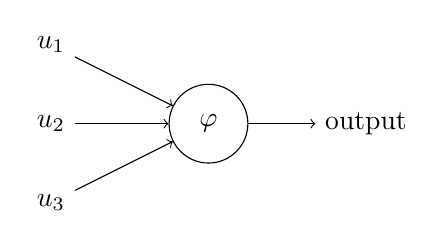
\begin{tikzpicture}[scale=1]

    \node[circle, draw, minimum size=1cm] at (0,0) (act) {$\varphi$};
    \node at (-2,  1) (u1) {$u_1$};
    \node at (-2, -0) (u2) {$u_2$};
    \node at (-2, -1) (u3) {$u_3$};
    \node at ( 2,  0) (out) {output};

    \path[draw, ->] (u1) edge (act) node {};
    \path[draw, ->] (u2) edge (act) node {};
    \path[draw, ->] (u3) edge (act) node {};
    \path[draw, ->] (act) edge (out) node {};

  \end{tikzpicture}
  \end{center}
}

\newcommand{\FeedForwardNet}[1]{
  \begin{center}
  \begin{tikzpicture}[scale=#1]
    \node[circle, draw, scale=#1] at (-1.5,0) (11) {};
    \node[circle, draw, scale=#1] at (-1.5,1) (12) {};
    \node[circle, draw, scale=#1] at (-1.5,2) (13) {};

    \foreach \n in {21, ..., 28}{
      \node[circle, draw, scale=#1] at (0, \n*.4 - 22*.4) (\n) {};
    }

    \foreach \idx in {11,...,13} {
      \foreach \jdx in {21,...,28} {
        \path[draw, ->] (\idx) edge (\jdx) node {};
      }
    }

    \node[circle, draw, scale=#1] at (1.5, 0.5) (31) {};
    \node[circle, draw, scale=#1] at (1.5, 1.5) (32) {};

    \foreach \idx in {21,...,28} {
      \foreach \jdx in {31,...,32} {
        \path[draw, ->] (\idx) edge (\jdx) node {};
      }
    }
  \end{tikzpicture}
  \end{center}
}

\newcommand{\RecurrentNet}{
  \begin{center}
  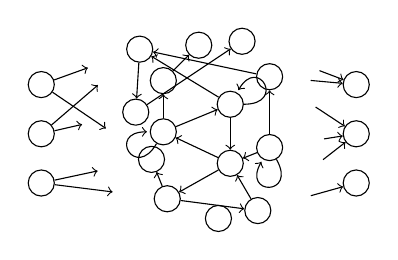
\begin{tikzpicture}[scale=.5]
    % input nodes
    \node[circle, draw] at (-1,1.5) (11) {};
    \node[circle, draw] at (-1,2.75) (12) {};
    \node[circle, draw] at (-1,4) (13) {};
    % reservoir nodes
    \node[circle, draw] at (2.2,1.1) (21) {};
    \node[circle, draw] at (4.5,0.8) (22) {};
    \node[circle, draw] at (4.8,2.4) (23) {};
    \node[circle, draw] at (1.4,3.3) (24) {};
    \node[circle, draw] at (2.1,2.8) (25) {};
    \node[circle, draw] at (3.8,3.5) (26) {};
    \node[circle, draw] at (4.8,4.2) (27) {};
    \node[circle, draw] at (1.5,4.9) (28) {};
    \node[circle, draw] at (2.1,4.1) (29) {};
    \node[circle, draw] at (3.8,2.0) (30) {};
    \node[circle, draw] at (3.5,0.6) (31) {};
    \node[circle, draw] at (3.0,5.0) (32) {};
    \node[circle, draw] at (4.1,5.1) (33) {};
    \node[circle, draw] at (1.8,2.1) (34) {};
    % output nodes
    \node[circle, draw] at (7,1.5)  (41) {};
    \node[circle, draw] at (7,2.75) (42) {};
    \node[circle, draw] at (7,4)    (43) {};

    % input connections
    \path[shorten >= 15pt, draw, ->] (12) edge (24) node {};
    \path[shorten >= 15pt, draw, ->] (12) edge (28) node {};
    \path[shorten >= 15pt, draw, ->] (11) edge (34) node {};
    \path[shorten >= 15pt, draw, ->] (11) edge (21) node {};
    \path[shorten >= 15pt, draw, ->] (13) edge (34) node {};
    \path[shorten >= 15pt, draw, ->] (13) edge (28) node {};
    % reservoir connections
    \path[draw, ->] (21) edge (22) node {};
    \path[draw, ->] (21) edge (34) node {};
    \path[draw, ->] (22) edge (30) node {};
    \path[draw, ->] (23) edge (30) node {};
    \path[draw, ->] (23) edge (27) node {};
    \path[draw, ->] (23) edge[in=-120, out=-60, loop] (23) node {};
    \path[draw, ->] (24) edge (33) node {};
    \path[draw, ->] (25) edge (26) node {};
    \path[draw, ->] (25) edge[in=-180, out=-120, loop] (25) node {};
    \path[draw, ->] (25) edge (29) node {};
    \path[draw, ->] (26) edge (28) node {};
    \path[draw, ->] (26) edge (30) node {};
    \path[draw, ->] (26) edge[in=60, out=0, loop] (26) node {};
    \path[draw, ->] (27) edge (28) node {};
    \path[draw, ->] (28) edge (24) node {};
    \path[draw, ->] (29) edge (32) node {};
    \path[draw, ->] (30) edge (25) node {};
    \path[draw, ->] (30) edge (21) node {};
    % output connections
    \path[shorten <= 10pt, draw, ->] (27) edge (43) node {};
    \path[shorten <= 15pt, draw, ->] (27) edge (42) node {};
    \path[shorten <= 15pt, draw, ->] (23) edge (42) node {};
    \path[shorten <= 15pt, draw, ->] (22) edge (41) node {};
    \path[shorten <= 25pt, draw, ->] (22) edge (42) node {};
    \path[shorten <= 25pt, draw, ->] (33) edge (43) node {};
    % output feedback paths
    %\draw[->] (41) -- (8.3, 1.5) -- (8.3, 6.7) -- (-2.3, 6.7) -- (-2.3, 1.5) -- (11);
    %\draw[->] (42) -- (8.1, 2.75) -- (8.1, 6.5) -- (-2.1, 6.5) -- (-2.1, 2.75) -- (12);
    %\draw[->] (43) -- (7.9, 4) -- (7.9, 6.3) -- (-1.9, 6.3) -- (-1.9, 4) -- (13);


  \end{tikzpicture}
  \end{center}
}

\newcommand{\RecurrentNetAnnotated}{
  \begin{center}
  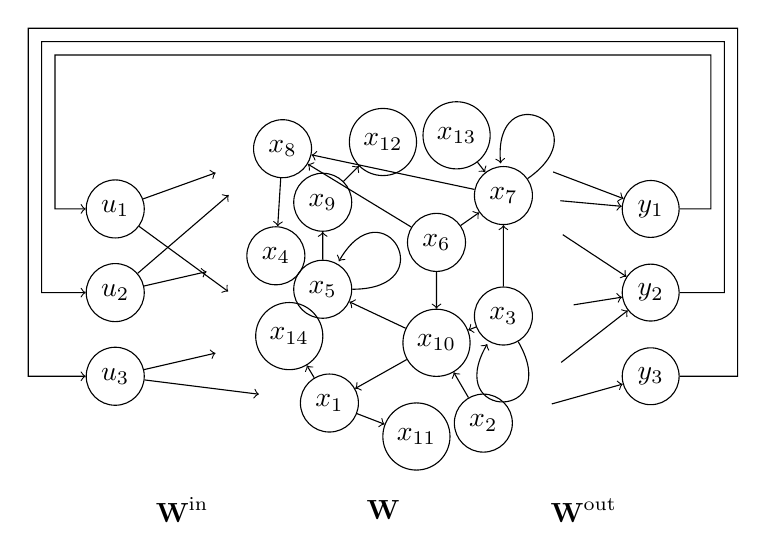
\begin{tikzpicture}[scale=.85]
    % annotations
    \node at ( 0, -0.5) (win) {$\textbf{W}^{\text{in}}$};
    \node at ( 3, -0.5) (w) {$\textbf{W}$};
   \node at ( 6, -0.5) (wout) {$\textbf{W}^{\text{out}}$};

    % input nodes
    \node[circle, draw] at (-1,1.5) (11)  {$u_{3}$};
    \node[circle, draw] at (-1,2.75) (12) {$u_{2}$};
    \node[circle, draw] at (-1,4) (13)    {$u_{1}$};
    % reservoir nodes
    \node[circle, draw] at (2.2,1.1) (21) {$x_{1}$};
    \node[circle, draw] at (4.5,0.8) (22) {$x_{2}$};
    \node[circle, draw] at (4.8,2.4) (23) {$x_{3}$};
    \node[circle, draw] at (1.4,3.3) (24) {$x_{4}$};
    \node[circle, draw] at (2.1,2.8) (25) {$x_{5}$};
    \node[circle, draw] at (3.8,3.5) (26) {$x_{6}$};
    \node[circle, draw] at (4.8,4.2) (27) {$x_{7}$};
    \node[circle, draw] at (1.5,4.9) (28) {$x_{8}$};
    \node[circle, draw] at (2.1,4.1) (29) {$x_{9}$};
    \node[circle, draw] at (3.8,2.0) (30) {$x_{10}$};
    \node[circle, draw] at (3.5,0.6) (31) {$x_{11}$};
    \node[circle, draw] at (3.0,5.0) (32) {$x_{12}$};
    \node[circle, draw] at (4.1,5.1) (33) {$x_{13}$};
    \node[circle, draw] at (1.6,2.1) (34) {$x_{14}$};
    % output nodes
    \node[circle, draw] at (7,1.5)  (41) {$y_{3}$};
    \node[circle, draw] at (7,2.75) (42) {$y_{2}$};
    \node[circle, draw] at (7,4)    (43) {$y_{1}$};

    % input connections
    \path[shorten >= 15pt, draw, ->] (12) edge (24) node {};
    \path[shorten >= 15pt, draw, ->] (12) edge (28) node {};
    \path[shorten >= 15pt, draw, ->] (11) edge (34) node {};
    \path[shorten >= 15pt, draw, ->] (11) edge (21) node {};
    \path[shorten >= 15pt, draw, ->] (13) edge (34) node {};
    \path[shorten >= 15pt, draw, ->] (13) edge (28) node {};
    % reservoir connections
    \path[draw, ->] (21) edge (31) node {};
    \path[draw, ->] (21) edge (34) node {};
    \path[draw, ->] (22) edge (30) node {};
    \path[draw, ->] (23) edge (30) node {};
    \path[draw, ->] (23) edge (27) node {};
    \path[draw, ->] (23) edge[in=-120, out=-60, loop] (23) node {};
    \path[draw, ->] (25) edge[in=60, out=0, loop] (25) node {};
    \path[draw, ->] (25) edge (29) node {};
    \path[draw, ->] (26) edge (28) node {};
    \path[draw, ->] (26) edge (30) node {};
    \path[draw, ->] (26) edge (27) node {};
    \path[draw, ->] (27) edge[in=95, out=35, loop] (27) node {};
    \path[draw, ->] (27) edge (28) node {};
    \path[draw, ->] (28) edge (24) node {};
    \path[draw, ->] (29) edge (32) node {};
    \path[draw, ->] (30) edge (25) node {};
    \path[draw, ->] (30) edge (21) node {};
    \path[draw, ->] (33) edge (27) node {};
    % output connections
    \path[shorten <= 10pt, draw, ->] (27) edge (43) node {};
    \path[shorten <= 15pt, draw, ->] (27) edge (42) node {};
    \path[shorten <= 15pt, draw, ->] (23) edge (42) node {};
    \path[shorten <= 15pt, draw, ->] (22) edge (41) node {};
    \path[shorten <= 25pt, draw, ->] (22) edge (42) node {};
    \path[shorten <= 25pt, draw, ->] (33) edge (43) node {};

    % output feedback paths
    \draw[->] (41) -- (8.3, 1.5) -- (8.3, 6.7) -- (-2.3, 6.7) -- (-2.3, 1.5) -- (11);
    \draw[->] (42) -- (8.1, 2.75) -- (8.1, 6.5) -- (-2.1, 6.5) -- (-2.1, 2.75) -- (12);
    \draw[->] (43) -- (7.9, 4) -- (7.9, 6.3) -- (-1.9, 6.3) -- (-1.9, 4) -- (13);

    %\draw[->] (7.9, 2.75) -- (8.5, 2.75) -- (8.5, 6.5)
    %  -- (-2.5, 6.5) -- (-2.5, 2.75) -- (-1.9, 2.75);
    %\draw (7.9, 1.2) -- (7.9, 4.3);
    %\draw (-1.9, 1.2) -- (-1.9, 4.3);

  \end{tikzpicture}
  \end{center}
}

\newcommand{\RNNFlowChart}{
  \begin{center}
  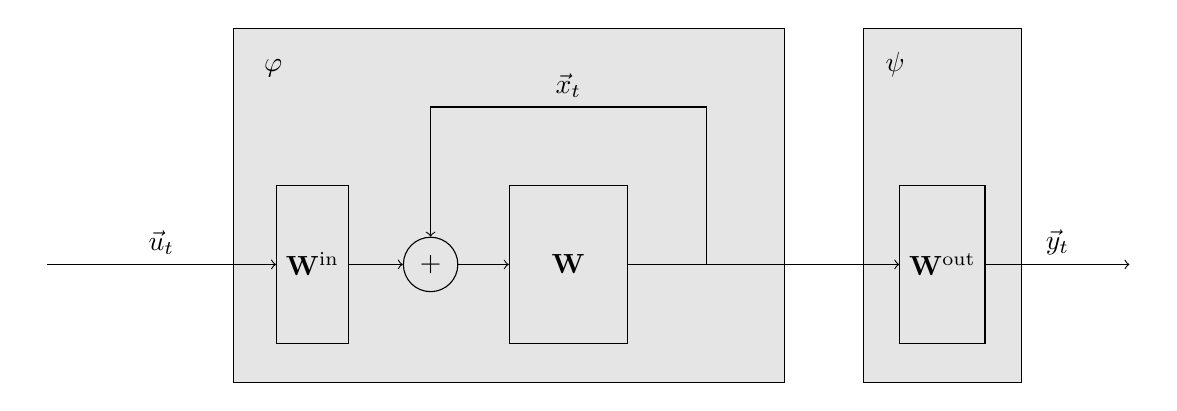
\begin{tikzpicture}[scale=1]
    \node[draw, rectangle,
          minimum width=7cm, minimum height=4.5cm,
          label={[shift={(-3,-.75)}]$\varphi$},
          fill=black!10,
          ] (Phi) at (4.5, 0.75) {};

    \node[draw, rectangle,
          minimum width=2cm, minimum height=4.5cm,
          label={[shift={(-.6,-.75)}]$\psi$},
          fill=black!10,
          ] (Psi) at (10, 0.75) {};

    \node (ut) at (-1.5,0) {};
    \node[draw, rectangle, minimum height=2cm]
        (Win) at (2,0) {$\mathbf{W}^{\text{in}}$};
    \node[draw, circle] (u+x) at (3.5,0) {+};
    \node[draw, rectangle, minimum height=2cm, minimum width=1.5cm]
        (W) at (5.25, 0) {$\mathbf{W}$};
    \node[draw, rectangle, minimum height=2cm] 
        (Wout) at (10,0) {$\mathbf{W}^{\text{out}}$};
    \node (yt) at (12.5, 0) {};

    \path[draw, ->] (ut) edge node[above] {$\vec{u}_t$} (Win);
    \path[draw, ->] (Win) edge (u+x) {};
    \path[draw, ->] (u+x) edge (W) {};
    \path[draw, ->] (W) edge (Wout) {};

    \path[draw, ->] (7, 0) -- (7, 2) 
        -- (5.25, 2) node[above] {$\vec{x}_t$} -- (3.5, 2) -- (u+x);
    \path[draw, ->] (Wout) edge node[above] {$\vec{y}_t$} (yt);
  \end{tikzpicture}
  \end{center}
}

\newcommand{\ESNFlowChart}{
  \begin{center}
  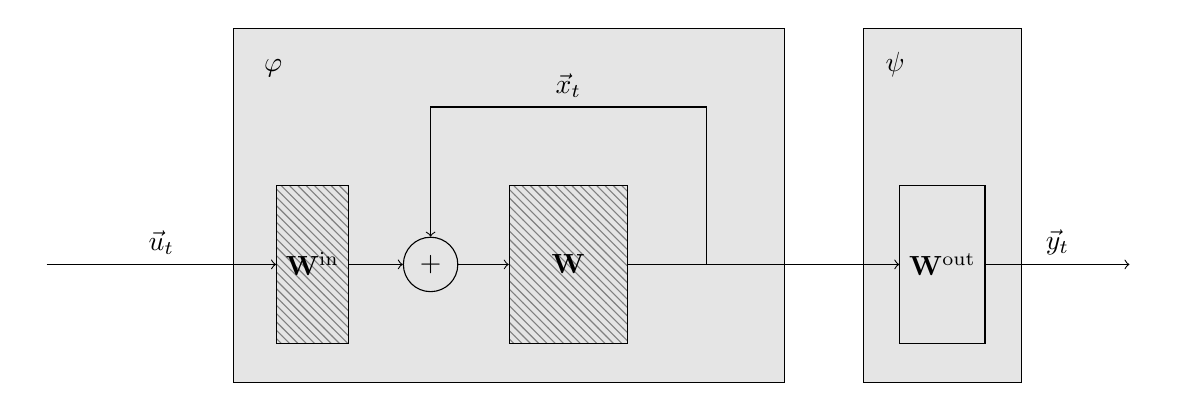
\begin{tikzpicture}[scale=1]
    \node[draw, rectangle,
          minimum width=7cm, minimum height=4.5cm,
          label={[shift={(-3,-.75)}]$\varphi$},
          fill=black!10,
          ] (Phi) at (4.5, 0.75) {};

    \node[draw, rectangle,
          minimum width=2cm, minimum height=4.5cm,
          label={[shift={(-.6,-.75)}]$\psi$},
          fill=black!10,
          ] (Psi) at (10, 0.75) {};

    \node (ut) at (-1.5,0) {};
    \node[draw, rectangle, minimum height=2cm,
          pattern=north west lines, pattern color=gray,
        ] (Win) at (2,0) {$\mathbf{W}^{\text{in}}$};
    \node[draw, circle] (u+x) at (3.5,0) {+};
    \node[draw, rectangle, minimum height=2cm, minimum width=1.5cm,
          pattern=north west lines, pattern color=gray,
        ] (W) at (5.25, 0) {$\mathbf{W}$};
    \node[draw, rectangle, minimum height=2cm] 
        (Wout) at (10,0) {$\mathbf{W}^{\text{out}}$};
    \node (yt) at (12.5, 0) {};

    \path[draw, ->] (ut) edge node[above] {$\vec{u}_t$} (Win);
    \path[draw, ->] (Win) edge (u+x) {};
    \path[draw, ->] (u+x) edge (W) {};
    \path[draw, ->] (W) edge (Wout) {};

    \path[draw, ->] (7, 0) -- (7, 2) 
        -- (5.25, 2) node[above] {$\vec{x}_t$} -- (3.5, 2) -- (u+x);
    \path[draw, ->] (Wout) edge node[above] {$\vec{y}_t$} (yt);
  \end{tikzpicture}
  \end{center}
}


% code listings
\usepackage[scaled=0.6]{beramono}
\usepackage{minted}
\usemintedstyle{tango}
\definecolor{bggrey}{rgb}{0.90, 0.90, 0.90}
\definecolor{bgwhite}{rgb}{1,1,1}
\setminted{bgcolor=bggrey, fontsize=\footnotesize, linenos, numbersep=-12pt}
% nice inline code
\makeatletter
\newcommand{\currentfontsize}{\fontsize{\f@size}{\f@baselineskip}\selectfont}
\makeatother
\setmintedinline{fontsize=\currentfontsize, bgcolor=bgwhite}
\newcommand{\ttt}[1]{\texttt{#1}}

% links in document
\usepackage{hyperref}
\renewcommand\UrlFont{\ttfamily\itshape}
\definecolor{linkblue}{rgb}{0.3, 0.3, 0.3}
\hypersetup{
  colorlinks=true,
  linkbordercolor=linkblue,
  pdfborderstyle={/S/U/W 1},
  linkcolor=linkblue,
  urlcolor=linkblue,
  allcolors=linkblue,
}

% show subsections in table
\setcounter{tocdepth}{2}


\begin{document}

\assignment{Master Thesis}
\author{Niklas Heim\\ September 4th, 2018}
\title{Automated Anomaly Detection \\ In Chaotic Time Series}
\subtitle{A Reservoir Computing Approach}
\frontpageimage{cover/gradient_cover.jpg}
\advisor{Professor Brian Vinter\\ Asst. Professor James E. Avery}
\institution{University of Copenhagen}
\department{Niels Bohr Institute}

\maketitle

\frontmatter
\pagestyle{ruledtitle}
\begin{vplace}[0.5]
\section*{Acknowledgements}%
\label{sec:acknowledgements}

I would like to express my gratitude to {\em eScience} and {\em TeamOcean}, the
two research groups at the University of Copenhagen that I was allowed to be
part of. Their Professors {\em Brian Vinter} and {\em Markus Jochum} have
provided a stimulating, collaborative environment for interesting research
which I have enjoyed and highly appreciated. Further I want to thank all the
group members, that always had an open ear for my countless questions and have
had a great influence on this thesis with their ideas and suggestions.
Especially, I want to thank {\em James Avery} who has provided a tremendous
amount of help, feedback, and inspiration during the whole duration of this
project without ever expecting anything in return.\\

A big thank you also goes to all my friends who have read and re-read this
thesis and made suggestions for improvements. Additionally, most of the visual
appeal of this work is owed to {\em Fabian Dornhecker} from the {\em BamOida
Interrogang\rlap?!} The cover image was drawn by a neural network at the
Wentworth Institute of Technology.\\

Finally I want to thank my parents for always supporting and encouraging me in 
my undertakings despite this `rather aberrant choice of a career'.
\end{vplace}

\cleardoublepage
\section*{Abstract}%
\label{sec:abstract}

The purpose of this study is to create a framework that is able to
automatically detect unusual behaviour in non-linear dynamical systems.  We
assume no prior information about the physics that govern these dynamics, so
there is no knowledge about the kind of anomaly that we are looking for.  This
is motivated by the large amounts of output that state of the art,
eddy-resolving ocean models produce.  These large datasets might contain
unknown physical behaviour, such as the recently discovered Kuroshio anomaly
(Sec.~\ref{sec:kuroshio}).  It is impossible for humans to evaluate all the
available climate model data within an acceptable time frame. An automated
anomaly detection is a first step towards harnessing the full potential of such
expensive simulations and could contribute to a deeper understanding of the
ocean circulation.\\

The detection problem is approached by trying to define what is normal, so that
everything that looks significantly different from this norm can be treated as
anomalous. This norm is found by predicting the future evolution of a system
that has been observed for a certain amount of time.  This is not a trivial
task, because non-linear systems can exhibit chaotic behaviour which makes
their prediction notoriously hard. However, it can be solved by employing a
special kind of recurrent neural network. Once the prediction is extracted from
the network, it can be compared to the true values of the dataset and where
they deviate significantly, a potential anomaly is found.

The type of recurrent network that is used is called \emph{echo state network}
and belongs to the class of \emph{reservoir computing} methods.  They feature a
comparatively low computational cost and have been shown to be able to predict
chaotic systems with surprising accuracy [\cite{pathak2018model}].\\

Concepts of machine learning and artificial intelligence are, despite their
proven effectiveness, still very sparsely utilized in climate research.
Therefore this work also serves as a showcase of what can be done by expanding
the set of standard analysis tools towards these methods.
The final result is the successful detection of the Kuroshio anomaly in the
turbulent ocean dataset.\\

\vfill
The code for the anomaly detection (\url{https://github.com/nmheim/torsk}) and
for this document (\url{https://github.com/nmheim/thesis}) can be found on
GitHub.

\begin{KeepFromToc}
\hypersetup{linkcolor=black}
\newpage\tableofcontents
\hypersetup{linkcolor=linkblue}
\end{KeepFromToc}

\mainmatter
\chapter{Introduction}
\label{cha:introduction}
\epigraph{
  \hypersetup{linkcolor=bgwhite}
  This thesis will explore the possibility of creating an anomaly detection for
  non-linear time series. In its broadest sense this means finding unusual,
  unexpected, or new patterns in a given dataset. In this introductory chapter,
  the motivation for searching for anomalous behaviour is described alongside
  the requirements for a general anomaly detection algorithm. Because many
  physical systems that are of interest for an outlier detection are non-linear
  and possibly even show \emph{chaotic} behaviour, a brief definition of
  chaotic time series is given, followed by three concrete exemplary datasets.\\
  The problem of detecting anomalies has been
  studied in many fields, which has lead to a great number of different
  approaches to the problem, some of which will be summarized in
  Chapter~\ref{cha:anomaly_detection};  Chapter~\ref{cha:neural_networks}
  introduces Neural Networks and their potential for predicting arbitrary time
  series, their implementation is described in Chapter~\ref{cha:implementation}
  and finally Chapter~\ref{cha:results} presents the so-called \emph{echo
  state network} applied to the three datasets that were introduced earlier.
  \hypersetup{linkcolor=linkblue}
}


\section{Motivation}
\label{sec:motivation}

The identification of unusual or aberrational behaviour is treated in many
other scientific fields:  The purpose of magnetic resonance imaging (MRI) is to
find tissues that are not expected to be found at a certain location in the
body, indicating a tumor. Biology studies genetic anomalies, \emph{mutations},
that can cause either illness or an increased chance of survival of an
individual.  Engineers monitor their equipment to detect early warning signs
before a machine breaks.  Banks try to identify fraudulent transactions based
on peculiarities in credit card data.  Anomalies in weather data can give early
hints on upcoming droughts, storms or other weather phenomena.  DNA sequence
mutations, engine monitoring, fraud detection, and weather data are examples of
sequential datasets that can be regarded as time series.  Detecting outliers in
time series can help prevent undesired behaviour or develop an early warning
systems.  With the growing amount of data that is being produced in many
different fields it becomes infeasible to manually analyze the given datasets.
It is therefore highly desirable to create an anomaly detection that is as
general as possible with regard to the data it can successfully process.\\

A field which could benefit immensely from an automated anomaly detection is
ocean modelling.  Large scale, high resolution simulations that cover the whole
Earth with more than 30 different variables such as temperature, velocity, and
density easily take up tens of gigabytes for a single time step. The vast
majority of the simulated ocean, much like the real ocean, is almost completely
unexplored.  Potentially unknown physical behaviour that could be hidden in
these datasets could be found by an automated outlier search. An example of
such an anomaly is the state changing ocean current called \emph{Kuroshio} on
the coast of Japan.  In irregular periods of several years it changes from an
elongated to a contracted state. This phenomenon has just recently come to the
attention of the scientific community and its origin is subject of vivid
debate. A detection of similar anomalies would be a very interesting finding in
itself, but it could also contribute to a deeper understanding of the Kuroshio
anomaly and the ocean circulation as a whole.

A large part of the anomaly detection model consists of a Neural Network. They
have been successfully applied to a very large number of different problems,
but have not yet found their way into the standard analysis tools of climate
scientists. With this thesis we hope show what could be achieved with an AI
driven approach to climate research.



\section{Defining Normality}%
\label{sec:defining_what_is_normal}

This thesis aims for the creation of an automatic detection algorithm that can
analyze large spatio-temporal datasets. We assume no prior knowledge about the
physics that produces the data, so there is no knowledge about the kind of
anomaly that we are looking for.  This requires to define what is
{\em normal}, so that everything that looks significantly different than this
norm can be treated as anomalous.  In time series this norm can be defined by
trying to predict the future evolution based on a previously observed history.
This means that we want to create a model that consumes an input sequence
$\mathbf{u}$ and returns a prediction sequence $\mathbf{y}$ (formal description
in Sec.~\ref{sub:prediction}):
\begin{equation}
  \mathbf{y} = F(\mathbf{u})
\end{equation}
The acquired prediction can subsequently be compared with the true values that
the sequence takes on for the predicted interval.  As soon as a reasonably good
prediction is made, the actual detection of an anomaly becomes quite simple.
Based on the degree of the deviation of prediction and truth, an \emph{normality
score} (Sec.~\ref{sub:anomaly_score}) can be calculated to define how large the
deviation must be in order to count as an anomaly.


\section{Applications}%
\label{sec:applications}

The generality of the algorithm is showcased with three exemplary datasets.
Each of the datasets will be described in more detail in the sections
\ref{sec:mackey_glass_system}-\ref{sec:kuroshio} of this chapter, but in short
they can be summarized as follows.

The first test-problem is a scalar chaotic system governed by the Mackey-Glass
equation. Scalar systems will further be referred to as zero-dimensional (0D).
%
Next, the algorithm is applied to a real-world example: climate records that
were obtained from Greenland ice-cores and include well known anomalies that
are called Dansgaard-Oeschger (DO) events.  The time series consists of two
markers that are fed to the detection algorithm, which is slightly increasing
the complexity of the task. The DO dataset can be regarded as a very small
one-dimensional (1D) system, as the input is a vector with two components.
%
Finally, the performance of the algorithm on a 2D system is analyzed. It
consists of a sequence of simulated sea surface height (SSH) images of the
previously mentioned Kuroshio region next to Japan. A successful anomaly
detection on this dataset would equate to an automated novelty detection in a
vast amount of climate data.



\section{Outline}%
\label{sec:outline}

The second chapter gives a brief introduction to what anomalies are, describes
some frequently used detection techniques, and defines the goal of the
predictive anomaly detection that will be used.  In the third chapter, whose
subject is Neural Networks, the theoretical background that is needed to
implement an automated time series prediction is laid out. It includes an
introduction to feedforward and recurrent networks before describing a new
machine learning concept called \emph{reservoir computing} (RC). The RC
approach, in comparison to traditional ML, is less computationally expensive
and was shown to be capable of forecasting chaotic systems surprisingly well in
a paper by [\cite{jaeger2004}] and for the first time for high dimensional
datasets by [\cite{pathak2018model}]. The implementation of the algorithm is
sketched in chapter~\ref{cha:implementation} and the results are presented in
chapter~\ref{cha:results}.


\newpage
\section{Chaotic Time Series}%
\label{sec:chaotic_time_series}

Time series are characterized by a chronological sequence of events.  In this
thesis only discrete time series, where each data point is associated with a
timestamp, are treated.  The basic components of a \emph{linear} time series are
level, trend, seasonal, and random effects. \emph{Level} is simply the current
value of the series, the \emph{trend} describes the increase and decrease from
one step to another. The \emph{seasonal} component refers to recurring patterns
that can be explained by some kind of seasonal influence like the tides.
\emph{Random} effects describe the statistical fluctuations of the series.
This is a typical linear treatment of the problem of analysing sequences.  The
complex problem is broken down into parts which can be solved individually and
finally linearly recombined.  For {\em non-linear} systems this cannot be done
so easily.  Various physical systems exhibit this non-linear behaviour which
can, under certain conditions, lead to \emph{chaotic} time series.
\begin{quote}{S. H. Strogatz}
  \emph{Chaos is aperiodic long-term behaviour in a deterministic system that
  exhibits sensitive dependence on initial conditions.}
\end{quote}
By aperiodic we mean behaviour that cannot be explained by strictly periodic
effects. There are no random inputs needed for this aperiodicity to occur,
which is suggested by the deterministic nature of the system. Its capricious
behaviour arises from the non-linearity.  The sensitivity to initial conditions
is the most commonly noted feature of chaotic systems.  It means that two
points $x(t)$ and $x(t)+\delta(t)$ that start out infinitesimally close to each
other will quickly diverge and evolve in completely different ways.  Their
separation may initially grow exponentially fast
\begin{equation}
  ||\delta(t)|| \sim ||\delta_0|| e^{\lambda t}.
\end{equation}

In this case the number $\lambda$ is called Lyapunov exponent. In systems where
$\lambda > 0$, one finds chaotic behaviour and the larger $\lambda$ grows the
more sensitive is the system to initial perturbations. The Lyapunov exponent
for the famous Lorenz attractor~[\cite{lorenz1963deterministic}] can be
computationally found to be $\lambda \approx 0.9$.  Chaotic systems are not the
same as \emph{unstable} systems, which also exhibit this sensitivity to initial
conditions. Unstable systems however, diverge towards infinity, while in
chaotic systems $\delta(t)$ is bounded by the radius of the \emph{attractor}.
A formal definition of attractors is out of the scope of this work, but the
interested reader may be referred to the book \emph{Non-linear Dynamics and
Chaos} by [\cite{strogatz}].


\newpage
\section{Mackey-Glass System}%
\label{sec:mackey_glass_system}

The Mackey-Glass (MG) system is a simple \emph{delay} differential equation,
that exhibits chaotic behaviour under certain conditions. It is studied
extensively in non-linear dynamics and serves as a benchmark for chaotic
prediction algorithms. It is defined by

\begin{equation}
  \label{eq:mackey_glass}
  \frac{\partial x}{\partial t} = \beta \frac{x_\tau}{1+x_\tau^n} - \gamma x,
  % discrete:
  %x(n+1) = x(n) + \delta (\frac{0.2x(n+\tau/\delta)}{(1+x(n-\tau/\delta)^{10}} - 0.1x(n))
\end{equation}

where $\beta$ and $\gamma$ are constants and $x_\tau$ denotes the value
$x(t-\tau)$, representing the delay.
\begin{figure}
  \centering
  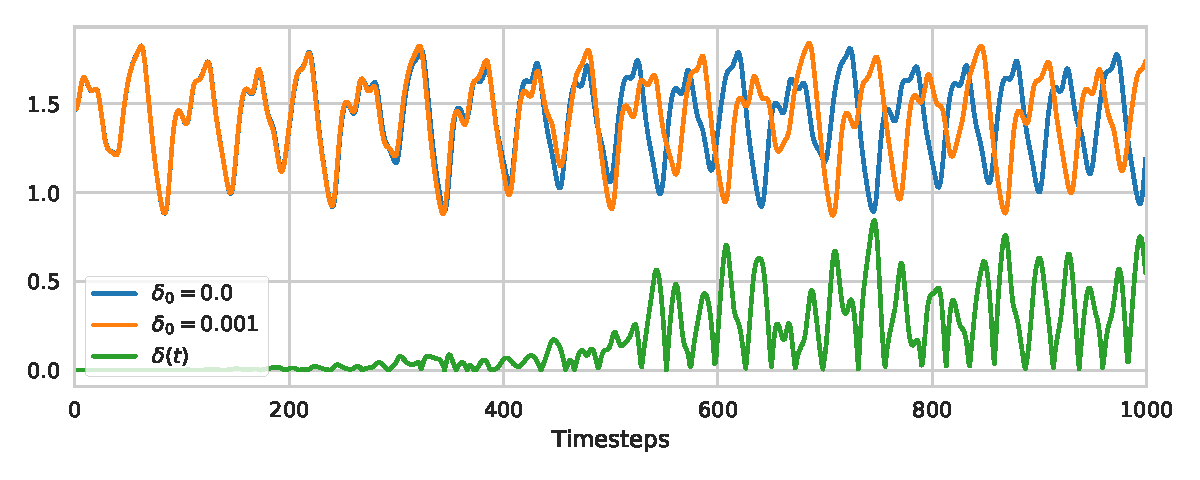
\includegraphics[width=\linewidth]{mackey_glass.pdf}
  \caption{Mackey-Glass time series created from Eq.~\ref{eq:mackey_glass}.  It
    nicely shows the aperiodic behaviour of chaotic time series, which makes it
    difficult to predict the next cycle. The two different evolutions are caused by
    a separation of $\delta_0 = 0.001$. There are no anomalies in the
    sequence. They will be introduced in Sec.~\ref{sec:res_mackey_glass_system}
    by slightly varying $\gamma$ over time.}
  \label{fig:mackey_glass}
\end{figure}
Two sequences that are created by solving Eq.~\ref{eq:mackey_glass} with the
values $\beta = 0.1$, $\gamma=0.2$ and a delay of $\tau=17$ are shown in
Fig.~\ref{fig:mackey_glass}. To solve the MG system initial values of the
length of the delay $\tau$ need to be specified. The two different evolutions
in the plot are created by slightly perturbing the initial values by
$\delta_0$. Additionally the plot shows how the separation $\delta(t)$ of the
two runs evolves. As expected, the peaks of the separation look very much like
an exponential for some time.
The local lyapunov exponent (LLE, [\cite{eckhardt1993}]) of the Mackey-Glass
system was calculated to LLE $\approx 0.01$ by [\cite{sprott}].



\newpage
\section{Dansgaard-Oeschger Events}%
\label{sec:dansgaard_oeschger_events}

During the last glacial period the North Atlantic region was subject to a
number of large climatic fluctuations known as Dansgaard-Oeschger (DO) events.
They describe abrupt increases in surface temperature of up to 15$^\circ$C over
a few decades, followed by a gradual cooling. Automatically detecting DO events
in time series that are obtained from Greenland ice-cores could serve as an
interesting benchmark for this anomaly detection method. Additionally the
dataset serves as a first step towards higher dimensional time series.

The INTIMATE project (INTegrating Ice-core, MArine, and TErrestrial records)
has recently managed to extract records of the DO events from Greenland
ice-cores that were drilled down to depths of about 3000m and contain climatic
information of the past 100 000 years.  Two different markers that clearly show
DO events are considered here: the so-called $\delta^{18}$O value is directly
linked to past temperatures, while the Ca$^{2+}$ concentration measures dust
content, which can be connected to atmospheric conditions such as the
atmosphere's circulation pattern.

The $\delta^{18}$O value measures the ratio of the lighter oxygen isotope
$^{16}$O and the heavier $^{18}$O in precipitation water [\cite{rasmussen2014}].
Higher temperatures aid the evaporation of water that contains the heavier
oxygen isotope, which means that roughly, one per mill change in $\delta^{18}$O
corresponds to a temperature difference of 1.5-4$^\circ$C.  With Greenland
ice-cores it is possible to resolve annual temperature oscillations as far back
in time as 8000 years. The sequence that is considered here contains annual
means because we are not interested in seasonal changes.

The concentration of Ca$^{2+}$ is essentially a measure of the dust content of
the ice. More dust indicates stronger winds that carried it to Greenland. By
measuring other isotopes it is even possible to determine where the dust comes
from, which gives hints on the atmospheric circulation patterns at the time,
but these isotopes are not considered here.  Fig.~\ref{fig:doevents} shows how
well the Ca$^{2+}$ and $\delta^{18}$O values coincide. Not that the time axis
shows age, so the time moves forward from right to left. The DO events are
indicated by the grey shaded regions.

\begin{figure}
  \centering
  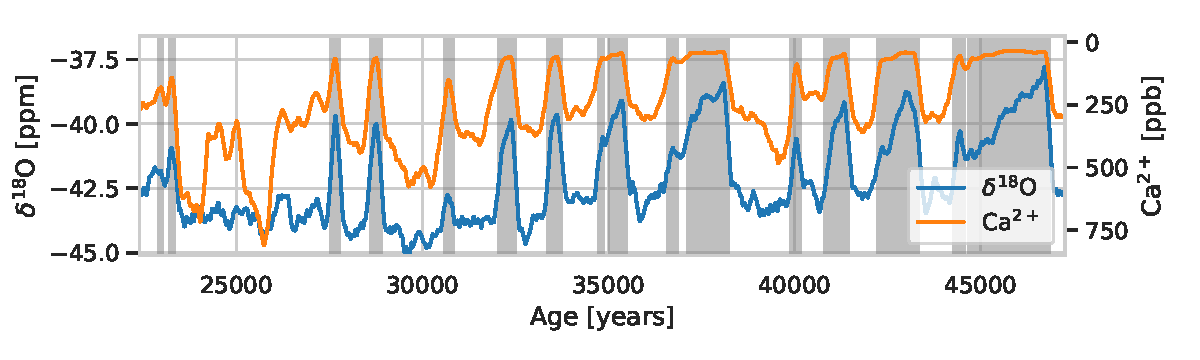
\includegraphics[width=\linewidth]{doevents.pdf}
  \caption{A sample of the $\delta^{18}$O (related to temperature) and
  Ca$^{2+}$ (dust content) sequences.  Dansgaard-Oeschger are marked by the
  grey shaded regions.}
  \label{fig:doevents}
\end{figure}



\newpage
\section{Kuroshio}%
\label{sec:kuroshio}

The Kuroshio [\textsc{japanese: black tide}] is one of the strongest ocean
boundary currents in the world and is the result of the western intensification
[\cite{pedlosky2013ocean}] of the ocean circulation in the North Pacific. The
3-day mean of simulated sea surface height (SSH) data
(Fig.~\ref{fig:kuroshio_snapshot}) shows the Kuroshio and its extension that
reaches into the North Pacific basin. It carries with it large amounts of
energy, nutrients and biological organisms, which have a large impact on the
local and global climate. To make itself even more relevant, the Kuroshio
exhibits a interesting and not yet understood phenomenon. In front of the coast
of Japan it oscillates between two distinct states
(Fig.~\ref{fig:kuroshio_elon_contr}): an elongated (right) and a contracted
state (left).  The transition between the two states typically takes one to two
years and occurs, as it seems, randomly every few years.  In 2017 it
transitioned to its elongated state for the first time in over a decade, as
reported by a Japanese newspaper [\cite{mainichi}]. To the interested reader it
also describes its impact on the local fishing industry as well as on tide
levels and the weather.

\begin{figure}
  \centering
  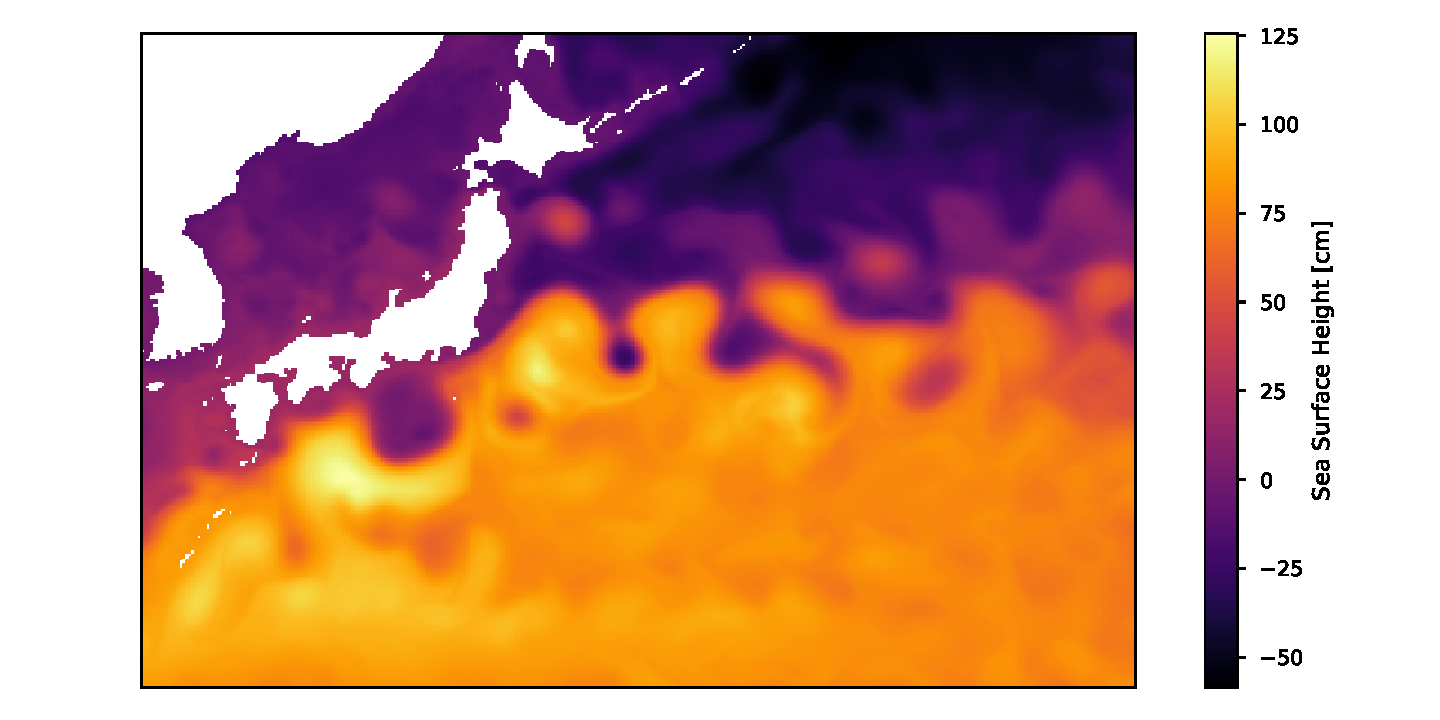
\includegraphics[width=1.05\linewidth]{kuroshio_snapshot.pdf}
  \caption{3-day mean of simulated sea surface height data. The Kuroshio is
  visible at the sharp transition between blue and yellow color. It flows along
  the coast of Japan before turning into the North Pacific basin. The figure is
  created by a 440x290 pixel window of the global simulation domain that is
  3600x2400 pixels large.}
  \label{fig:kuroshio_snapshot}
\end{figure}

The simulations that created the pictures were carried out by \emph{Team Ocean}
at the University of Copenhagen. The \emph{Community Earth System Model} (CESM)
was used to simulate the global domain with a horizontal resolution of
0.1$^\circ$ and 62 depth layers. It writes out 3-day means for all variables,
but in this work only the SSH fields are considered, which results in
images of a total size of 3600 x 2400 pixels. A more detailed
description of the experimental setup can be found in [\cite{poulsen2018}].  As
indicated by Fig.~\ref{fig:kuroshio_elon_contr}, the Kuroshio anomaly was
reproduced in the CESM simulations. The two plots of the elongated and the
contracted state were produced by averaging 200 3-day mean snapshots of the
simulation at different time periods. Taking the difference of them should give
us an intuition for how a successful anomaly detection should look like.\\
\begin{figure}
  \centering
  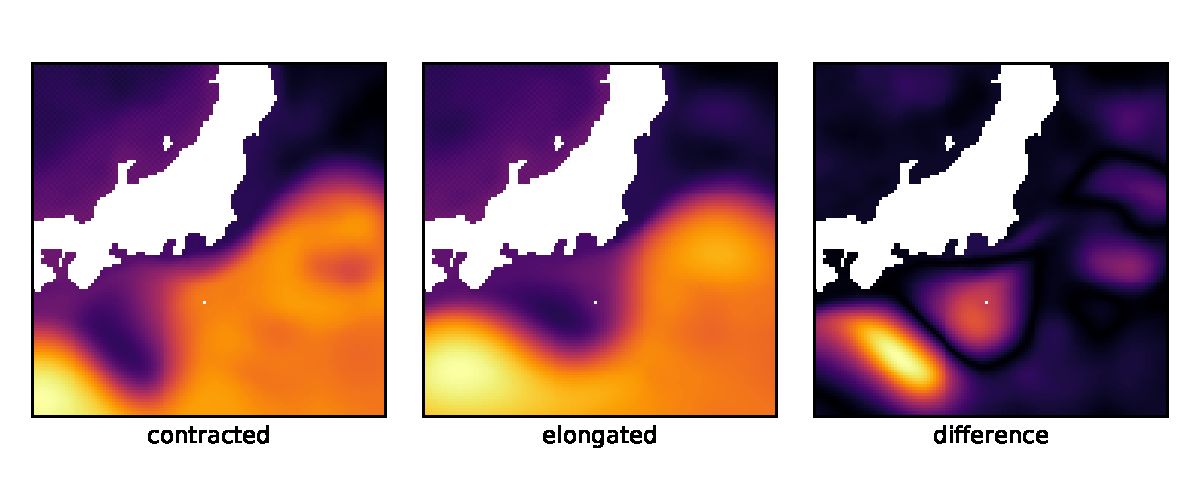
\includegraphics[width=\linewidth]{kuroshio_elon_contr.pdf}
  \caption{The two distinct states of the Kuroshio created by averaging SSH over
  two years. The images have a size of 100 x 100 which are sliced out of the global
  simulation domain of 3600 x 2400 pixels.}
  \label{fig:kuroshio_elon_contr}
\end{figure}

\begin{figure}
  \centering
  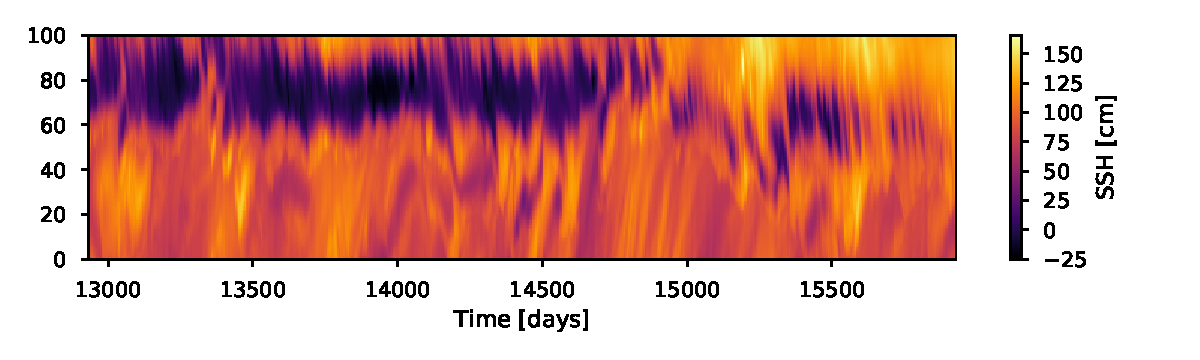
\includegraphics[width=\linewidth]{kuroshio_evolution.pdf}
  \caption{A row of the southern SSH field from
  Fig.~\ref{fig:kuroshio_elon_contr} over time.  The Kuroshio anomaly where
  the stream transitions from contracted to elongated state is visible between
  day 14500 and 15000.
  }
  \label{fig:kuroshio_evolution}
\end{figure}

Detecting the state changes of the Kuroshio with an automated anomaly search
could be the first step in creating a way of finding novel behaviour in the
vast amount of climate model output, which is essentially as unexplored as the
oceans of our real world.  Such novelties could, apart from their potential of
displaying new physical processes, contribute both to a further understanding
of the behaviour of the Kuroshio itself and the ocean circulation patterns as a
whole.  The automatic detection of the Kuroshio anomaly would mark a major step
towards a creation of an algorithm that could find anomalies in noisy and
turbulent datasets such as ocean simulations.

\chapter{Anomaly Detection}
\label{cha:anomaly_detection}
\epigraph{
  The field of anomaly detection is very broad and many different fields have
  developed a great variation of different methods for finding outliers.  This
  work is focusing on detecting anomalies in sequences by predicting the
  expected evolution of a time series and comparing this prediction to real
  observations (or simply: the truth).  Before describing this process in more
  detail, this chapter defines the different kinds of anomalies that exist in
  sequences and briefly summarizes two other, common detection methods
  for sequence outlier detection.
}

\section{Anomalies}
\label{sec:anomalies}
An anomaly (or outlier) refers to a pattern in a dataset that does not match
an expected behaviour.
In time series, there are two basic types of anomalies:
\begin{enumerate}

  \item \emph{Simple anomalies}, describe instances that can be considered as
    an outlier only with respect to their value. This is the most basic kind of
    anomaly which can easily be caught by ordinary, statistical, range-based
    detection algorithms. The anomaly in Fig.~\ref{fig:intro_point_anomaly}
    consists of a single instance and is hence called a \emph{point} anomaly.
    \begin{figure}
      \centering
      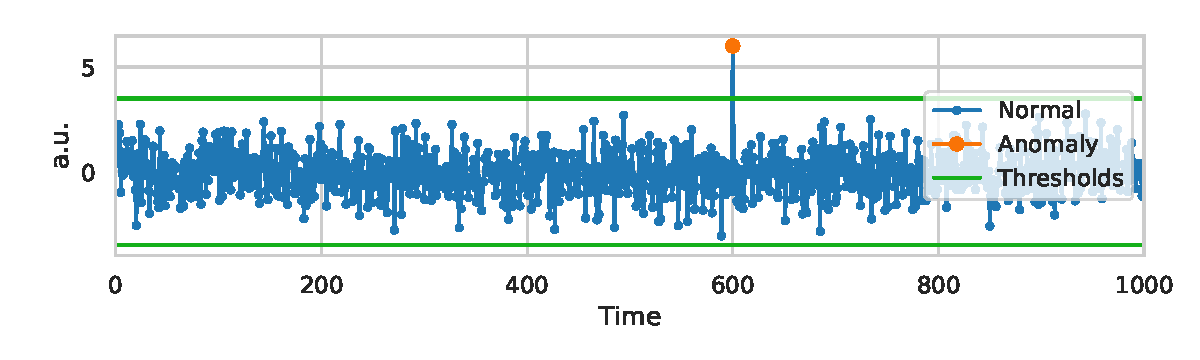
\includegraphics[width=\linewidth]{intro_point_anomaly.pdf}
      \caption{The simple point anomaly can easily be detected by appropriate
      thresholds (green lines).}
      \label{fig:intro_point_anomaly}
    \end{figure}

  \item \emph{Contextual anomalies} are patterns that are only anomalous within
    a certain context, but not otherwise. In time series, the context is
    provided by two attributes: The \emph{contextual attribute} is typically
    time itself, while the \emph{behavioural attributes} describe the actual
    values of the examined dataset. Fig.~\ref{fig:intro_context_anomaly} shows
    a contextual anomaly consisting of several abnormal points, which is
    referred to as a \emph{discord} or \emph{subsequence} anomaly.
    \begin{figure}
      \centering
      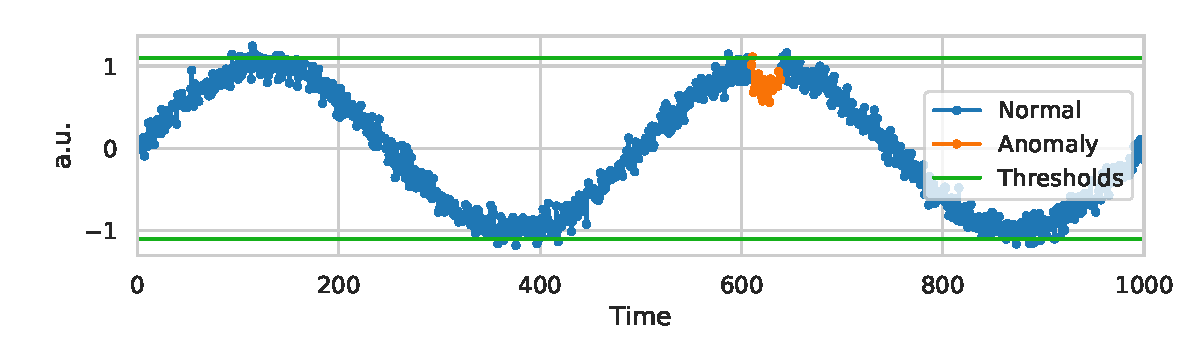
\includegraphics[width=\linewidth]{intro_context_anomaly.pdf}
      \caption{Contextual anomalies are not detectable with simple statistical
      methods without causing a large number of false positives.}
      \label{fig:intro_context_anomaly}
    \end{figure}
\end{enumerate}


\newpage
\section{Techniques}
\label{sec:techniques}

The difficulty of anomaly detection stems from the fact that the patterns that
are searched for are typically not known.  Different fields have come up with a
large number of different approaches for the detection of the different kinds
of anomalies. Two such approaches  are sketched below: \emph{proximity-based}
techniques, and {\em information theoretical} approaches [\cite{AggarwalCharuC2017}].

\subsection{Proximity-based Anomaly Detection}
\label{sub:proximity_based_anomaly_detection}

By applying certain transformations to segments of a time series, a segment can be
mapped into a multidimensional vector space. The proximity can then be
calculated for example with the Euclidean distance, which opens up the whole
range of proximity-based outlier detection methods, such as cluster, distance,
and density based techniques.

The trivial example of such a transformation is to just consider segments of
length $n$ as a vector of length $n$.  Other approaches include \emph{Discrete
Fourier Transforms} (DFT) or \emph{Discrete Wavelet Transforms} (DWT), the
simplest of which is the \emph{Haar Wavelet}. A Haar Wavelet decomposition is
sketched in Fig.~\ref{fig:haar_wavelets}, a more detailed description of how
wavelet transformations work is given in [\cite{AggarwalCharuC2017}]. The
advantage of transforming a sequence into a vector of wavelet coefficients is
that the coefficients directly represent short-term and long-term dependencies.
This enables a reduction of the dimensionality of the space that has to be
analyzed depending on the nature of the problem. For example, frequencies above
a certain threshold can be ignored.  The application of proximity-based methods
naturally becomes much more effective on the transformed sequences. Depending
on the nature of the dataset different transformations are more effective.  For
sequences with dominant periodic parts the DFT works better, while series with
discontinuities are well represented by the Haar-DWT.

\begin{figure}
  \centering
  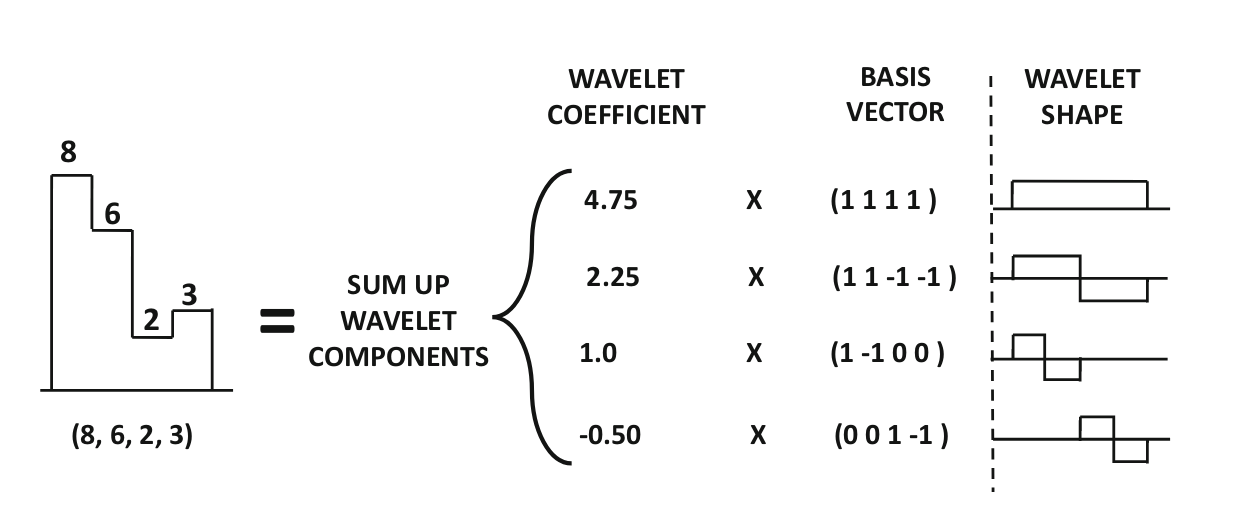
\includegraphics[width=0.9\linewidth]{haar_wavelets.png}
  \caption{Haar wavelet decomposition of series of length $N=4$.
  [\cite{AggarwalCharuC2017}]}
  \label{fig:haar_wavelets}
\end{figure}


\subsection{Information Theoretical Approaches}
\label{sub:information_theoretical_approaches}

Information theoretical models rely on the creation of so-called
\emph{summaries} of a dataset. The length of the summary is shorter the simpler
the sequence is.  A completely periodic sequence can be described very
concisely.  Sequences that contain anomalies require a longer description,
hence the summary becomes longer. An anomaly is defined as a point or
subsequence that leads to a large increase of the length of the summary.  In
practice, measures such as entropy can take the part of the summary length. The
entropy of a sequence $X$ is defined by:

\begin{equation}
  H(X) = - \sum_{x \in X} P(x) \log P(x),
\end{equation}

where $P(x)$ is the probability of a value $x$.



\subsection{Prediction}
\label{sub:prediction}

The approach that is used in this thesis relies on modelling the normal
behaviour of the given dataset and creating predictions. The predictions can
then be compared to the actual values of the series, essentially reducing the
problem to a \emph{simple anomaly}, which can be detected by a simple threshold
on the error.\\
Considering a time series of length $T$, the single input \emph{frames} of a
series will further be denoted by $\vt{u}$ with $t \in [0,T]$.  An input frame
contains all the features at time $t$ and is represented by a vector with $m$
components, which could be the pixel values of a flattened image.  The same
holds for the target frames $\vt{d}$, which hold the desired output at every
time step. The output of the forecasting algorithm is called the prediction,
denoted by $\vt{y}$, and ought to be as close as possible to the target
$\vt{d}$.  Prediction and target frames can have a different size from the
input frames:

\begin{align}
  \vt{u} &= (u^t_1, u^t_2, ..., u^t_m)^T, \nonumber\\
  \vt{d} &= (d^t_1, d^t_2, ..., d^t_k)^T. \\
  \vt{y} &= (y^t_1, y^t_2, ..., y^t_k)^T. \nonumber
\end{align}

By defining an input sequence $\textbf{u}$ as a sequence of vectors

\begin{equation}
  \textbf{u} := (\vec{u}_0, \vec{u}_1, \vec{u}_2, ..., \vec{u}_M)
\end{equation}

the prediction problem can be formulated by finding a function $F$, that
returns a good estimate $\textbf{y}$ of the next $N$ true vectors $\textbf{d}
:= (\vec{u}_{M+1}, ..., \vec{u}_{M+N})$.

\begin{equation}
  \textbf{y} = (\vec{y}_{M+1}, ..., \vec{y}_{M+N}) 
             = F(\vec{u}_0, \vec{u}_1, ..., \vec{u}_M)
             = F(\textbf{u})
\end{equation}

The approximation of the function $F$ is a regression problem which has
been studied intensively throughout history [\cite{narx_prediction}].
Recently, Neural Networks (NN) have been applied to anomaly detection, as they
can model certain non-linear sequences without a priori knowledge about the
data, just by applying a learning algorithm. An in depth explanation of how NNs
can be applied to find $F$ for spatio-temporal datasets is given in
Chapter~\ref{cha:neural_networks}.  Before 1980, time series were typically
predicted by using autoregressive, moving-average models (ARMA), which where
introduced by [\cite{boxjenkins}].  Another method published by
[\cite{winters1960forecasting}] on forecasting sales improved Holt`s double
exponential smoothing.  This method later became known as the Holt-Winters
method.  Both approaches are described in in the next paragraphs.  It should be
noted though that they are both linear regression models, which makes them
incapable of predicting non-linear time series. For the sake of simplicity they
are described only for the case of scalar time series.\\

During the regression (or training) phase of the forecasting algorithm the
target for the prediction is typically the true observation of the next time
step $\vt{d} = \vec{u}_{t+1}$.  The parameters of the algorithm are tuned until
the predictions $\vt{y}$ are good enough.  As soon as the `one step ahead'
prediction problem is solved, predictions further into the future can be made
by feeding $\vt{y}$ back to the algorithm as the next input $\vec{u}_{t+1}$. In
this case the algorithm is in the forecasting phase and is not optimized
any more. This prevents information about the next frame to leak into the
prediction process.

\begin{figure}
  \centering
  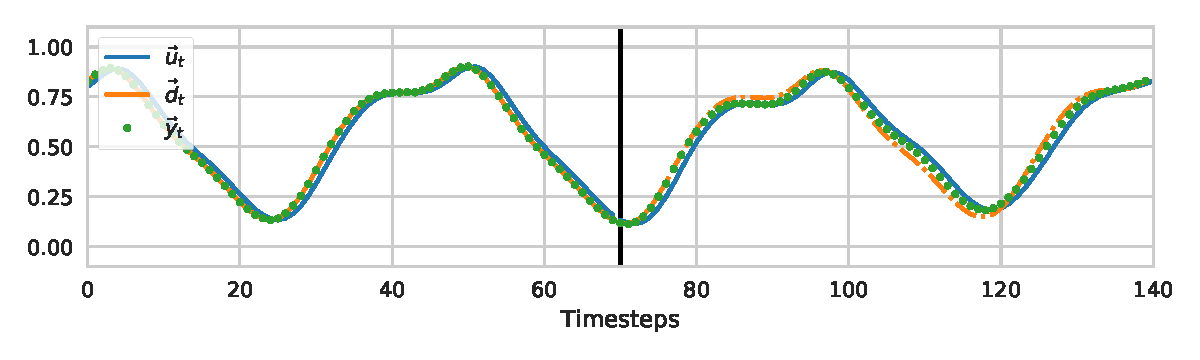
\includegraphics[width=\linewidth]{train_predict_mode.pdf}
  \caption{Input $\vt{u}$, target $\vt{d}$, and prediction $\vt{y}$ during the
  regression phase (left of the black line) and during the prediction phase.
  In the prediction phase the algorithm has no access to the true target
  any more, which is why they are depicted by a dashed line.}
  \label{fig:train_predict_mode}
\end{figure}

\subsubsection{Auto-regressive Integrated Moving Average}
\label{sub:arma}

Auto-regressive integrated moving average (ARIMA) models are widely used in
forecasting and are typically applied to non-stationary time series.  A
non-seasonal ARIMA model is defined by three parameters $p$, $q$, and $d$.  The
first parameter $p$ is the order of the auto-regressive (AR) model, $q$ is the
order of the moving-average (MA) model, and $d$ is the number of non-seasonal
differences that are needed to obtain a stationary time series.  This means
that $Y_t$ is the result of applying the sequence difference operator $\Delta
y_t = y_{t+1}-y_{t}$ for $d$ times to $y_t$:
\begin{equation}
  Y_t = \Delta^d y_t = \sum_{k=0}^d (-1)^{d-k} \binom{d}{k} y_{t+k}
\end{equation}

With the difference $Y_t$ we can write the general forcasting equation of the
ARIMA model:
\begin{equation}
  y_t = \mu + \sum_{i=1}^p \varphi_i Y_{t-i} + \sum_{i=1}^q \theta_i \epsilon_{t-i}
\end{equation}

where $\mu$ is the mean of the series, $\varphi_i$ are the $p$ parameters of
the AR model, $\theta_i$ the parameters of the MA model, and $\epsilon_i$ white
noise error terms.  The parameters of the MA and AR models have to be fit to
the data and the order of the difference must chosen a priori.


\subsubsection{Holt-Winters Method}
\label{sub:holt_winters_method}

The Holt-Winters method belongs to the class of exponential smoothing
algorithms.  In contrast to MA models that apply the same weights over a window
of a time series, exponential smoothing uses exponentially decaying weights
back in time.

The most basic form is called simple exponential smoothing (SES), where the
level of previous points provides an estimate for the next time step.  The
method maintains an estimated point $\vt{y}$, which is calculated based on
previous points and estimates.  They are assigned weights, which decrease
exponentially going back in time.
\begin{align}
  y_t = \alpha d_t + (1-\alpha)y_{t-1}
\end{align}
The smoothing parameter $\alpha$ determines exponentially
decreasing weights that are applied to previous data points.  The smoothing
parameter is chosen such that the mean squared error of prediction and data
point is minimized.

The Holt-Winters method extends the SES approach from only forecasting the level
to smoothing equations for trend $b_t$ and seasonal $s_t$.
It is described by the following four equations:
\begin{align}
  l_t &= \alpha(d_t - s_{t-L}) + (1-\alpha)(y_{t-1} + b_{t-1}) &\text{level} \\
  b_t &= \beta(l_t - l_{t-1}) + (1-\beta)b_{t-1} &\text{trend} \\
  s_t &= \gamma(y_t - l_t) + (1 - \gamma)s_{t-L} &\text{seasonal} \\
  y_{t+m} &= l_t + m b_t + s_{t-L+1+(m-1) \bmod L} &\text{forecast}
\end{align}

where $L$ is the length of the seasonal component, $\alpha$, $\beta$, $\gamma$
are constants that need to be fit to the data and $m$ denotes how far into
the future the prediction goes.


\subsection{Anomaly Score}%
\label{sub:anomaly_score}

\begin{figure}
  \centering
  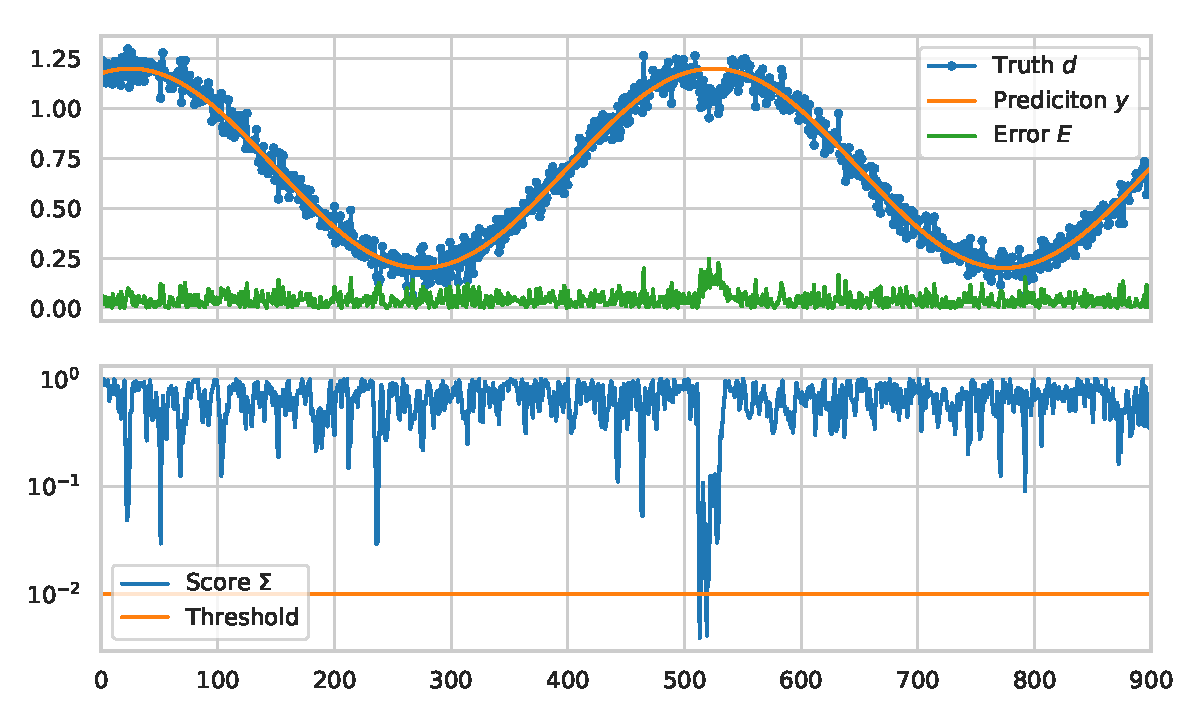
\includegraphics[width=\linewidth]{anomaly_score.pdf}
  \caption{With a good prediction $y$, the problem can be reduced to a simple
    anomaly detection over the error sequence $E$ (upper plot). The error
    sequence still takes on arbitrary values and can be converted into a
    probability of normality with an anomaly score (lower plot).
    The normality is calculated with sliding windows of length 100 for $\mu_E$
    and a length of 5 for $\mu_e$.
  }
  \label{fig:anomaly_score}
\end{figure}

With the predicted sequence $\textbf{y}$ it becomes quite simple to detect an
outlier, because the problem can be reduced to a \emph{simple anomaly} by
calculating the absolute error sequence $E$.

\begin{equation}
  \label{eq:err_seq}
  E_i = || \vt{y} - \vt{d} ||_2
\end{equation}

The error can now be thresholded to detect an anomaly, but the value of this
threshold depends on the specific dataset that is being analyzed.  To obtain a
probability for how anomalous a point or subsequence is, an \emph{anomaly
score} $\Sigma$ is defined as suggested by [\cite{numenta_realtime}]:

\begin{equation}
  \label{eq:normality_score}
  \Sigma = 1 - \text{erf}\bigg(\frac{\mu_e - \mu_E}{\sqrt{2}\sigma_E}\bigg),
\end{equation}

where $\mu_E$ and $\sigma_E$ denote the mean and standard deviation of a window
of length $N$ of the error sequence $E$. The mean $\mu_e$ is calculated from a
smaller subsequence of $E$ of length $n \ll N$. If $\mu_e$ is close to $\mu_E$
then $\Sigma$ will be close to one, and can thus be considered \emph{normal}
with a high probability. If $\mu_e$ and $\mu_E$ are far apart, the probability
of normality is low and the point becomes more likely to be an
outlier. This results in a score for the whole sequence, which can be used as
an intuitive threshold according to the problem at hand.
Fig.~\ref{fig:anomaly_score} shows how the anomaly detection problem of a
contextual outlier is first reduced to a simple anomaly by calculating $E$ and
then detected with a threshold on $\Sigma$. 

If the quantities $\vt{y}$ and $\vt{d}$ are vectors or matrices it might be
desirable to know which components in the vector (matrix) caused the anomaly.
For such a spatially resolved anomaly score the norm from Eq.~\ref{eq:err_seq}
can be removed and $\Sigma$ is calculated component-wise for every
coefficient in $|\vt{y} - \vt{d}|$.

\chapter{Neural Networks}
\label{cha:neural_networks}
\epigraph{In the recent years Neural Networks (NN) have solved more and more
  tasks that have previously been too difficult or simply too tedious to solve
  with traditionally coded algorithms. They have been successfully applied to a
  variety of problems such as pattern recognition, image classification and
  prediction.  As the NN algorithms learn from data, they seem to be good
  candidates for finding anomalies without any prior knowledge about the
  given dataset, as long as it is big enough. By applying online learning
  algorithms that learn and adapt continuously it should in theory be possible
  to create an automated, adaptive outlier detection.\\ This chapter describes
  the mechanics of NNs from the ground up. Starting with the widely used
  \emph{feedforward networks} (FNN), we go on to \emph{recurrent neural nets}
  (RNN). Similar to biological neural networks, they have cyclic connections,
  and are capable of processing sequences. After that, a special kind of RNN is
  introduced, that dramatically cuts computational costs and solves some
  notorious problems that arise during RNN training. In addition to the general
  difficulty of training NNs, they often rely on hyper-parameters, that are
  typically set by manually tuning the network.  This chapter is closed with a
  brief description of hyper-parameter optimization techniques which were used
  to automate this task.
}

\section{Feedforward Neural Networks}
\label{sec:feedforward_neural_networks}

The idea for artificial neural networks is based on the human brain,
which is a highly complex, non-linear, and parallel computer.  Just like the
brain, neural networks are constructed from small units that are connected to each other
with weights. In analogy to its biological counterpart these units are also
called \emph{neurons}. Older literature also often refers to them as
\emph{perceptrons}.  They are capable of processing and passing on incoming
information.
Traditional \emph{feedforward neural networks} (FNN) implement static
input-output mappings, which mathematically makes them pure functions of the
input signals. Figure \ref{fig:perceptron} shows a simple schematic of a single
neuron.  It generally has $n$ inputs $u_j$ and one output.  Each of the inputs
has an assigned weight $w_j$, which determines the contribution of a given
input to the output.  The output of a neuron will further be referred to as
\emph{activation} $y$:
\begin{equation}
  \label{eq:ffn_eq}
  y = \varphi \left( \sum_j (w_j u_j) + b  \right)
       = \varphi (\vec{w} \cdot \vt{u} + b).
\end{equation}
The sum over all the inputs multiplied by their weights can conveniently be
represented by a dot product.  Often a bias term $b$ is included, which can be
taken as a measure of how easy it is to activate the neuron.  The function
$\varphi$ is called activation function and can have various different forms,
from a simple binary function to an arbitrary (non-linear), monotonically
increasing function.  A frequently used activation function in FNNs is the
sigmoid function
\begin{equation}
  \sigma (z) = \frac{1}{1 + e^{-z}},
\end{equation}
which is shown in Fig.~\ref{fig:sigmoid}. To create a \emph{layer} of neurons
they are simply stacked on top of each other:
\begin{equation}
  \vt{y} = \varphi (\wmatr{} \vt{u} + \vec{b}).
\end{equation}

\begin{figure}
  \begin{minipage}{.42\textwidth}
    \centering
    \Perceptron
    \vspace{4.5mm}
    \caption{Schematic of a neuron [\cite{Nielsen2015}].
    The activation function is represented by the circle.}
    \label{fig:perceptron}
  \end{minipage}
  \hspace{.02\textwidth}
  \begin{minipage}{.54\textwidth}
    \centering
    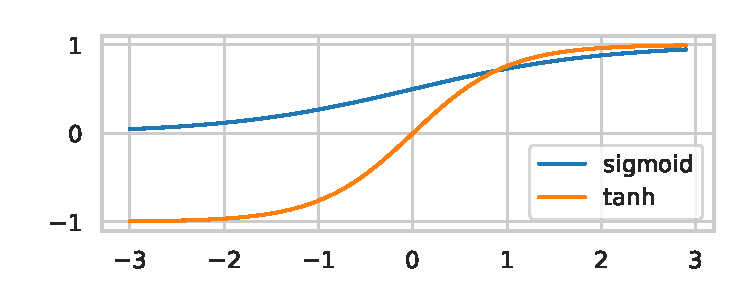
\includegraphics[width=\linewidth]{sigmoid_tanh.pdf}
    \caption{Sigmoid function $\varphi$. Typically used as an activation function
    in feedforward neural nets.}
    \label{fig:sigmoid}
  \end{minipage}
\end{figure}

The final FNN with multiple layers (such as in
Fig.~\ref{fig:feedforward_network}) is created by feeding the output of one
layer to another one until the last layer of the network is reached.  The
\emph{universal approximation theorem} [\cite{uni_approx_theorem}] states the
ability of FNNs to approximate an arbitrary non-linear function $f$
\begin{equation}
   \vt{d} = f(\vt{u})
\end{equation}
with arbitrary precision. This means that given any $\epsilon > 0$ we can find
an FNN $F$, such that
\begin{equation}
  ||F(\Theta, \vt{u}) - f(\vt{u})||_2 < \epsilon
\end{equation}

for all possible inputs $\vt{u}$. The exact form of the approximation $F$
depends on the network architecture, but generally it depends on a set of
parameters $\Theta$ called weights (and biases), which represent several layers
of the FNN.  Of course, the universal approximation theorem does not say
anything about the practical learnability of a task, which will be discussed in
Sec.~\ref{sub:gradient_descent}.

Each layer of an FNN can be represented by a matrix, and therefore only has the
computational expressibility of linear functions. This linearity is only broken
by the activation function. Without the non-linear activation an arbitrary
number of layers would not be more effective than a single one.  Through the
organization in layers FNNs are able to model not only arbitrary functions but
also to separate datasets that are not linearly separable.
Fig.~\ref{fig:feedforward_network} shows an FNN where the first (input) layer
represents the data that is fed into the network, followed by one or more
hidden layers, and an output layer.  Hidden layers act as a non-linear
transform that distorts the input in such a way that its classes become
linearly separable by the output layer.  An interactive explanation of how this
works can be found in a blog post by [\cite{colah_topology}].

\begin{figure}
  \centering
  \FeedForwardNet{2}
  \caption{Fully connected feedforward neural network with a single hidden
    layer and two output neurons.}
  \label{fig:feedforward_network}
\end{figure}

Every network that has more than two or three hidden layers is typically called
a \emph{deep neural network}. It is fundamentally not different from the basic
architecture of the described feedforward networks but holds the potential of
more powerful transformations of the input. The type of neural network that is
shown in Fig.~\ref{fig:feedforward_network} is called \emph{feedforward
network}, because the input data is entering the network at the input layer and
then passed through the network towards the output layer.  Feedforward nets are
often applied to classification tasks, such as the recognition of a certain
shape in an image.

The goal of the machine learning approach is to find a weight configuration
that captures the \emph{essence} of the presented dataset, meaning that it
generalizes well, including over inputs that it has not been trained with.
This is typically approached by some variation of Gradient Descent (GD). GD
algorithms try to minimize a certain loss or cost function with respect to a
given weight configuration (more detailed description in
Sec.~\ref{sub:gradient_descent}).  However, the pursued generalization of the
network is highly dependent on the training dataset. It should ideally include
the total variability of possible inputs.  This is very hard to achieve in
practice and the available datasets are typically split randomly into three
categories: \emph{training}, \emph{validation}, and \emph{test} set.  The
training set is used to optimize the network. Its loss is minimized by a GD
algorithm. The validation set is used to determine the performance of the
network on inputs that are not included in the training set.  The optimization
should be stopped as soon as the error on the validation set is not decreasing
any more in order to reduce the risk of overfitting. This is one of many
regularization methods that are applied in ML in order to achieve a
generalization over previously unseen datapoints. Because the information of
the validation set is leaking into the network via the early stopping
criterion, a third dataset is needed to evaluate the actual performance and
generalization of the network.  This third set is called the test set.

Feedforward networks outperform conventional algorithms at tasks such as image
recognition and other classification and pattern recognition.  They are,
however, not very suitable to model time series, as they cannot model correlations
of previous inputs. This means that they are not designed for the prediction of
sequences.  To be able to process sequences and make predictions,
\emph{recurrent} weight connections are introduced in
Sec.~\ref{sec:recurrent_neural_networks}.  Despite the compelling results that
can be achieved by FNNs, they have a few drawbacks.  Backpropagation algorithms
typically need very large amounts of data to train the network. The gradient
descent steps have to be small enough to not jump over the desired minima,
which leads to very long training times.  Additionally the nature of the
training data can lead to biases of the resulting network if it does not
properly represent the possible parameter space.  It is hard to infer
afterwards how the network came to a specific result, as the weight matrices do
not represent a traceable way of reasoning or logic.  A trained network is like
a black box, which does not come with an obvious way of determining how or why
a certain classification was made.


\subsection{Convolutional Neural Nets}%
\label{sub:convolutional_neural_nets}

A breakthrough in image classification performance was achieved by the
introduction of a subtype of FNNs, the \emph{convolutional neural networks}
(CNN), which can leverage the spatial structure of the input data.  They
combine the concept of filters from signal processing with the ML approach by
learning their own filters (often referred to as kernels as well) for feature
detection in images.  The convolutional operation of a given filter $F$ and an
image $H$ is defined by:
\begin{align}
  G &= H * F \text{, where}\\
  G[i,j] &= \sum_{u=-k}^k \sum_{v=-k}^k H[i-u, j-v]F[u,v]
\end{align}

A well known example of a filter for edge detection looks like this:
\begin{equation}
  F = \begin{bmatrix} 
    -1 & -1 & -1 \\ 
    -1 & 8  & -1 \\ 
    -1 & -1 & -1  
  \end{bmatrix}
\end{equation}

Applying it to a (black and white) image $H$
\begin{equation}
  H = \begin{bmatrix}
	  1 & 1 & 1 & 1 & 1 & 0 & 0 & 0 & 0\\
	  1 & 1 & 1 & 1 & 1 & 0 & 0 & 0 & 0\\
	  1 & 1 & 1 & 1 & 1 & 0 & 0 & 0 & 0\\
	  1 & 1 & 1 & 1 & 1 & 0 & 0 & 0 & 0\\
	  1 & 1 & 1 & 1 & 1 & 0 & 0 & 0 & 0\\
	  1 & 1 & 1 & 1 & 1 & 0 & 0 & 0 & 0\\
	\end{bmatrix}
\end{equation}

and padding the convoluted image $G$ to obtain the original dimensions results
in a filtered image $R$, which is zero everywhere except at the location of the
edge:

\begin{equation}
  \newcommand{\nan}{-}
  \newcommand{\minus}{\text{-}}
	R = \begin{bmatrix}
    \nan & \nan & \nan & \nan & \nan & \nan  & \nan & \nan & \nan\\
    \nan & 0 & 0 & 0 & 3 & \minus 3 & 0 & 0 & \nan\\
    \nan & 0 & 0 & 0 & 3 & \minus 3 & 0 & 0 & \nan\\
    \nan & 0 & 0 & 0 & 3 & \minus 3 & 0 & 0 & \nan\\
    \nan & 0 & 0 & 0 & 3 & \minus 3 & 0 & 0 & \nan\\
    \nan & \nan & \nan & \nan & \nan & \nan  & \nan & \nan & \nan\\
  \end{bmatrix}
\end{equation}

A convolutional layer consists of multiple kernels, which are learned via GD.
Each kernel can be thought of as a neuron that sees only a small part of the
input image at a time and slides over the whole image. Its output therefore
represents the local structure of said part of the image, which makes
a CNN capable of exploiting spatial structures in images (see schematic in
Fig.~\ref{fig:conv_layer}).  The kernels which are sliding over the input
images naturally lead to a translation invariance of the learned patterns
[\cite{lecun1995convolutional}]. A pattern that is recognized by a filter in one
region of the image can just as well be detected somewhere else, which stands
in contrast to fully connected layers for which the same pattern in different
parts of an image looks completely different.  Scale invariance can be achieved
by using multiple kernels of different size.  Feedforward nets, which are fully
connected to the input cannot leverage the spatial information as efficiently.
Additionally, CNNs decrease the number of parameters in comparison to a normal
FNN, which reduces the risk of overfitting and thus leads to a better
generalization of NNs.
\begin{figure}
  \centering
  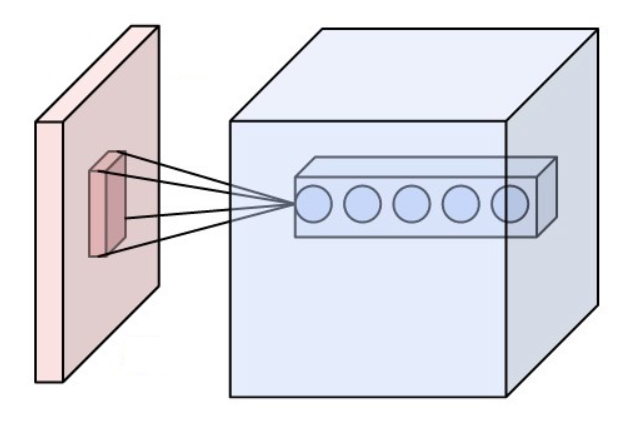
\includegraphics[width=0.4\linewidth]{conv_layer.png}
  \caption{The 2D input image on the left is transformed into a 3D output
  volume by applying multiple convolutions to the input [\cite{conv_layer_wiki}].}
  \label{fig:conv_layer}
\end{figure}

An interesting example of a CNN outside the realm of image classification is
AtomNet [\cite{dzamba1510atomnet}], which is used to predict bioactivity of
molecules for drug discovery by exploiting the local structure of biochemical
interactions.


\subsection{Gradient Descent}
\label{sub:gradient_descent}

The most common technique to train neural networks is Gradient Descent.
It is based on minimizing a \emph{loss} (cost or penalty) function $\mathcal{L}$
\begin{equation}
  \label{eq:batch_loss}
  \mathcal{L}(\Theta) = \sum_{\vt{u} \in \mathcal{U}} 
                        ||F(\Theta, \vt{u}) - \vt{d}||_2,
\end{equation}
which defines how close the network is to producing the
desired results.  The loss function that is used throughout this thesis is
given by Eq.~\ref{eq:batch_loss}, where the target outputs, given a certain
input $\vec{u}$ out of all training examples $\mathcal{U}$, are denoted by
$\vt{d}$.  

Initially, the weights of the network are set randomly and are to be adjusted
in the optimization phase, also called learning or training.  The loss is, of
course, dependent on all the weights and biases, which is where the gradient
descent comes into play.  The partial derivatives of the loss function are
taken with respect to all the weight and biases of the network to find the
gradient which points in the direction of steepest descent.  With this
calculated direction we can step the weights towards the nearest local minimum
and like that gradually increase the performance of the network.
\begin{equation}
  \label{eq:gradient_descent}
  \Theta' = \Theta + \eta \dd{\mathcal{L}}{\Theta}
\end{equation}
The size of the steps is defined by the \emph{learning rate} $\eta$, which has
to be chosen carefully.  If it is too large, the algorithm will oscillate
around the desired minimum, but if chosen too small, the training times will
become too long.  Several adaptive gradient computation algorithms address this
issue. One promising algorithm is called \emph{Adam} (Adaptive Moment
Estimation). Adam combines adaptive gradient descent methods with
momentum based algorithms [\cite{ADAM}]. Momentum-based optimizers add a fraction
of the previously used weight update to simulate an acceleration of the
gradient descent.  The method of applying the gradient descent algorithm to
multi-layer (deep) neural networks is called \emph{backpropagation} (BP),
because the gradient calculation is started at the last layer and iteratively
propagated back through the whole network by applying the chain rule. A more
detailed description of BP is given in Sec.~\ref{sub:backpropagation}.

There are three different variations of gradient descent, which only differ in
the way the sum in Eq.~\ref{eq:batch_loss} is interpreted.  Summing over all
available training examples $\vt{u}$, namely the whole \emph{batch}, is called
{\em batch GD}. Calculating the loss only for a single randomly chosen example,
is called \emph{stochastic gradient descent} (SGD). The compromise of the two,
mini-batch GD, uses a subset of the training examples, performs a weight
update, and then goes on to the next mini-batch.  Both stochastic and
mini-batch GD end up calculating an approximate loss $L$ from a subset $U
\subset \mathcal{U}$:
\begin{equation}
  \mathcal{L}(\Theta) \approx L(\Theta) = 
    \sum_{\vt{u} \in U} ||F(\Theta, \vt{u}) - \vt{d}||_2,
\end{equation}

which also leads to an approximated gradient. The updates that are performed
with the approximate gradient are hoped to enable the optimizer to jump out of
shallow local minima and saddle points, which is discussed further in the next
paragraph.

\subsubsection{Local Minima of the Error Surface}%
\label{ssub:local_minima_of_the_error_surface}

As BP is a gradient-based method, there is no guarantee at all, that the
algorithm will find the global minimum of the error surface.  To illustrate
this, Fig.~\ref{fig:error_surface_bgd} depicts a two dimensional error surface
with a global and a local minimum.  Depending on where on the surface the
optimization is started, it ends up in the local or global minimum.  It was
shown that for linear activation functions, the error surface contains only a
single minimum, the global one, with all other locations of zero gradient being
saddle points [\cite{BALDI}]. Momentum-based optimizers can find the global
minimum quite efficiently in such cases. However, this cannot be generalized to
the practically used NNs that almost exclusively use non-linear activations.
Optimizers that include momentum like the Adam optimizer can still sometimes
yield better results, as depicted in Fig.~\ref{fig:error_surface_bgd}.  The two
plots both show a two dimensional error surface, where the coordinates $x$ and
$y$ are regarded as the weights that have to be optimized.  The black, dotted
lines show different runs with varying initial values of $x$ and $y$.  The left
plot shows the convergence paths of plain batch GD algorithm as described
above, which converges towards the global minimum in three out of five cases.
As GD is a purely gradient based method, the path always advances in the
direction of steepest descent.  With the more advanced Adam optimizer, the
global minimum is found in four out of five cases. The momentum towards the
global minimum that is gained in the beginning carries the optimization away
from the local minimum.  Of course there are numerous cases where this approach
will not yield a global minimum. Additionally the Adam algorithm is much more
computationally expensive than plain GD and needs more steps, as can be seen
from the denser dots on the black lines.
\begin{figure}
  \begin{minipage}[b]{.49\textwidth}
    \centering
    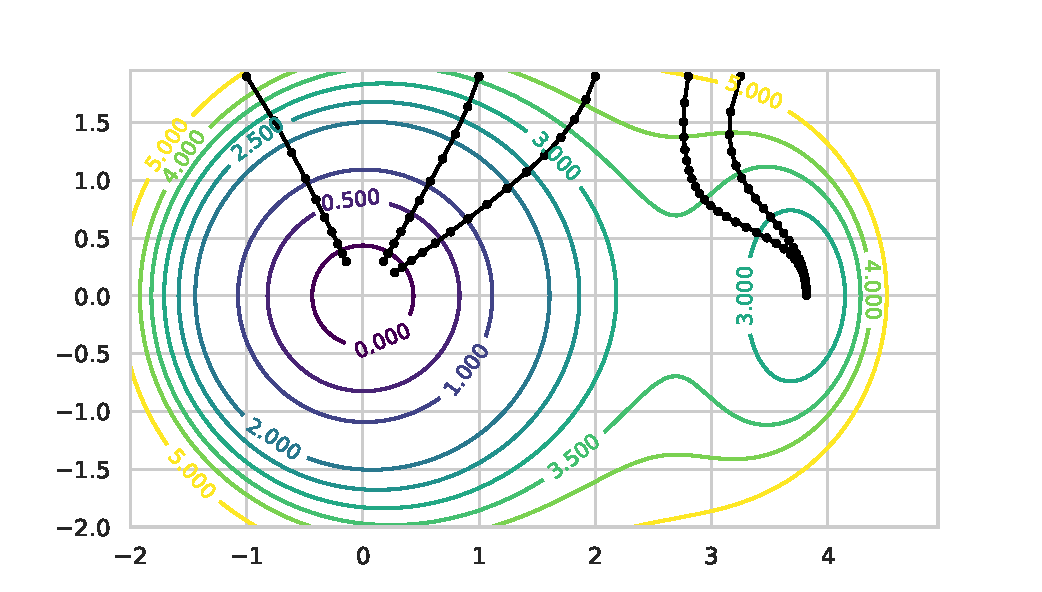
\includegraphics[width=\textwidth]{gradient_descent.pdf}
    GD
  \end{minipage}
  \hspace{.02\textwidth}
  \begin{minipage}[b]{.49\textwidth}
    \centering
    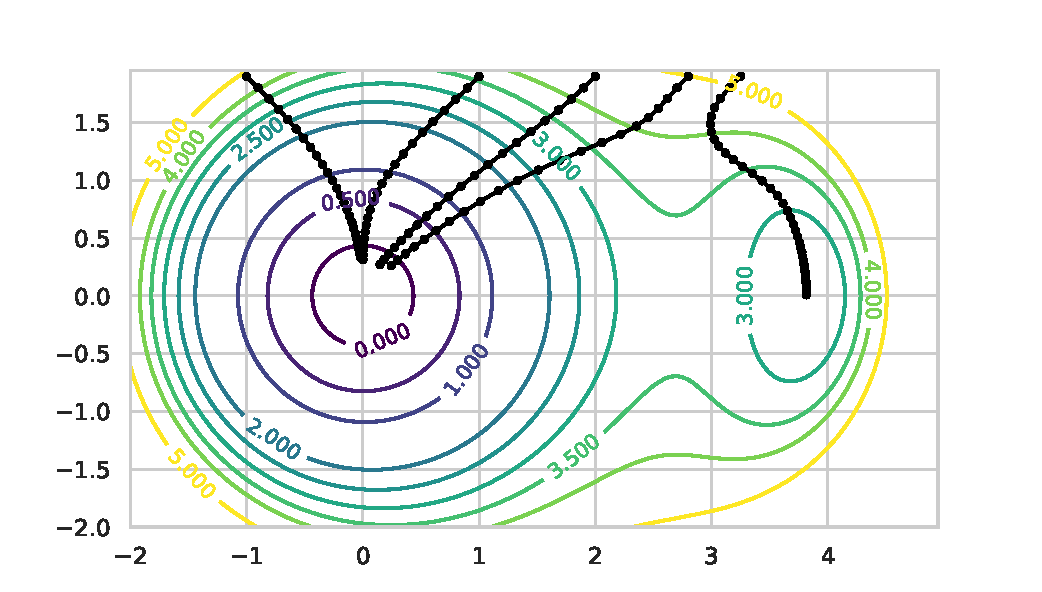
\includegraphics[width=\textwidth]{adam.pdf}
    Adam
  \end{minipage}
  \caption{On the left we can see a plain GD optimizer while on the right the
    Adam optimizer was used.  Depending on the starting values of the two
    variables, there are cases in which the optimization ends in the local
    minimum on the right. The GD optimizer needs fewer steps, while Adam finds
    the global minimum in one more case.}
  \label{fig:error_surface_bgd}
\end{figure}

\begin{figure}
  \begin{minipage}[b]{.49\textwidth}
    \centering
    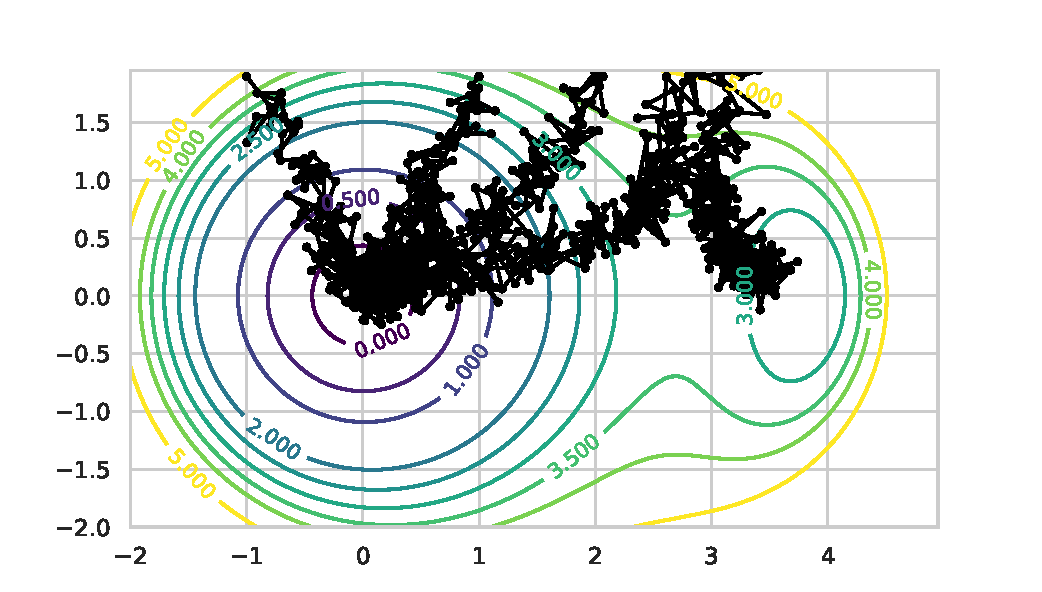
\includegraphics[width=\textwidth]{stochastic_gradient_descent.pdf}
    stochastic GD
  \end{minipage}
  \hspace{.02\textwidth}
  \begin{minipage}[b]{.49\textwidth}
    \centering
    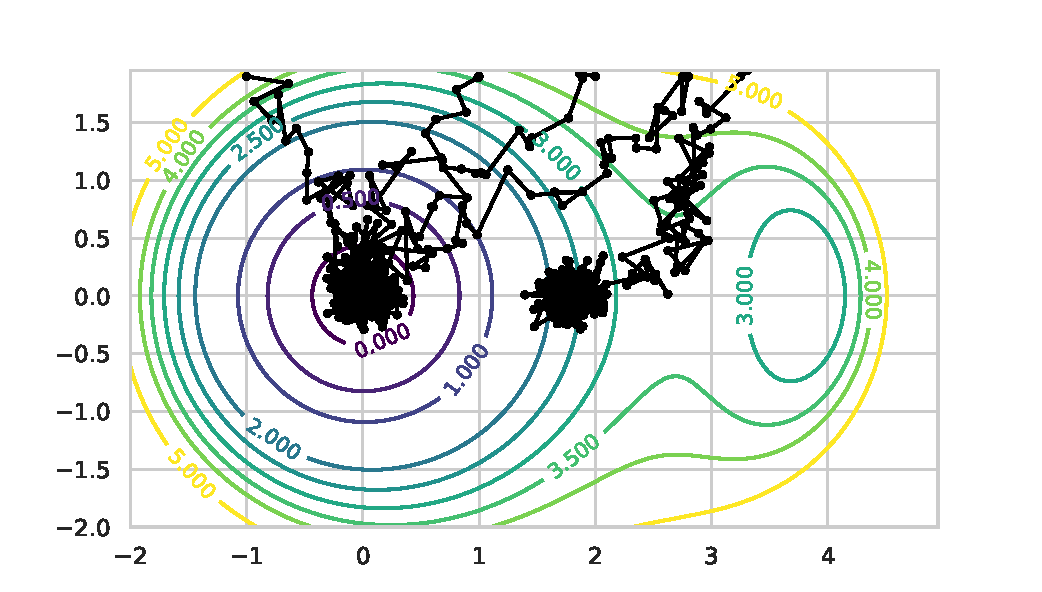
\includegraphics[width=\textwidth]{stochastic_adam.pdf}
    stochastic Adam
  \end{minipage}
  \caption{Convergence paths of stochastic GD algorithms. The noisy paths are
    due to the approximation of the gradient through mini-batches.}
  \label{fig:error_surface_sgd}
\end{figure}
To date, the most commonly used technique to encourage GD to converge to the
global minimum is mini-batch gradient descent.  Instead of evaluating the
\emph{true} loss of the whole training set as indicated by
Eq.~\ref{eq:batch_loss}, SGD adapts the weights after every mini-batch $X$.
This leads to an approximation of the gradient and causes oscillations in the
convergence path, which should make it more probable to escape local minima.
Fig.~\ref{fig:error_surface_sgd} again compares plain GD and Adam, but now with
the perturbing effect of evaluating an approximate loss. The number of training
steps that have to be taken increase significantly, but plain SGD is able to
find the global minimum in four out of five cases. Stochastic Adam almost
reaches the minimum in all five cases, but seems to get stuck right before
the global minimum in the last case.  The conclusion we can draw from the above
examples is that care has to be taken with respect to the convergence of NNs.
Different optimizers, gradient descent variations, and initializations can
yield vastly different results. However, experience has shown that in most
pattern recognition tasks, SGD algorithms can find a local minimum that yields
satisfactory performance, even though it is not guaranteed that this minimum is
global.  In most applications, an increase in the network connections is
supposed to create paths around suboptimal local minima [\cite{rumelhart1986}].
Additionally, in most applications the training is actually stopped early,
meaning at the time the validation error does not decrease further.  This is
done because a network that is fitted perfectly to the training data would most
probably not generalize well over new inputs.  In most cases it is therefore
acceptable or even desirable to remain in a \emph{good} local minimum that
results in a good generalization of the network.


\subsection{Backpropagation}%
\label{sub:backpropagation}

Backpropagation is the basic algorithm that carries out the GD minimizations
that were introduced previously. It was invented in the 1970s but not widely
used until the paper by~[\cite{rumelhart1986}], which marks a breakthrough in the
field of machine learning.  For an easy to read but in depth description of the
subtleties of BP the reader is referred to the book \emph{Neural Networks and
Deep Learning} by [\cite{Nielsen2015}].

Fundamentally, BP is nothing more than the application of the chain rule to the
cost function of a neural network, which can be solved by an \emph{automatic
differentiation} (AD) algorithm. In fact, BP is a special case of AD called
\emph{reverse mode} AD~[\cite{autodiff}].  To illustrate the BP algorithm we will
consider a network with $L$ feedforward layers, where the activations of the
first layer are just the inputs to the network ($\vec{u} = \vec{y}_1$) and the
last layer contains the network outputs $\vec{y}_L$. The components $y^j_l$ of
the vector $\vec{y}_l$ that contains all activations of a layer $l$ are
calculated based on the previous layer:
\begin{equation}
\begin{aligned}
  z^j_l &= \sum_k w^{jk}_l y^k_{l-1} + b^k_L \\
  y^j_l &= \varphi(z^k_l) \label{eq:forward_pass},
\end{aligned}
\end{equation}
where $\vec{z}_l$ are called the \emph{weighted inputs}.  The system above may
be altered such that a given activation depends on any \emph{previous} layer
activation, but \emph{not} on activations of any \emph{next} layer. This step is
named \emph{forward pass}.  During the forward pass, all activations are
calculated starting from the first layer. The goal of the \emph{backward pass}
is to adjust all the weights $w^{jk}_l$ (and biases $b^k_L$) such that the loss $L$
\begin{equation}
  L = \frac{1}{2}\sum_k (d^k - y^k_L)^2
\end{equation}
of a single input example $\vec{u}$ is minimized. BP solves this by iteratively
calculating the gradients needed for Eq.~\ref{eq:gradient_descent} starting
from the last layer.  Before directly calculating the necessary gradients it is
easier to compute the \emph{error} $\delta_L$ of the weighted inputs for each
unit $j$ of the last layer:
\begin{equation}
  \delta^j_L = \dd{L}{z^j_L} = \frac{1}{2}\sum_k \dd{}{z^j_L}(d^k - y^k_L)^2
             = \dd{L}{y^j_L}\dd{y^j_L}{z^j_L}
             = (d^j - y^j_L) \varphi'(z^j_L) \label{eq:delta_last_layer},
\end{equation}
where the sum vanishes because $y^k_L$ only depends on $z^j_L$ if $j = k$.
Now the error of any layer $l$ can be expressed in terms of the error of the
next layer $l+1$:
\begin{equation}
  \delta^j_{l} = \dd{L}{z^j_l} = \sum_k \dd{L}{z^j_{l+1}}\dd{z^j_{l+1}}{z^j_l}
  = \sum_k \delta^j_{l+1} \dd{z^j_{l+1}}{z^j_l}
  = \sum_k \delta^j_{l+1} w^{kj}_{l+1} \varphi'(z^j_l). \label{eq:delta_other_layer}
\end{equation}

The desired error gradients can be found to be:
\begin{equation}
\begin{aligned}
  \dd{L}{b^j_l} &= \delta^j_l, \\
  \dd{L}{w^{jk}_l} &= y^j_{l-1} \delta^j_l. \label{eq:error_grads}
\end{aligned}
\end{equation}
They can be used to incrementally update the weights and biases according
to Eq.~\ref{eq:gradient_descent}.

\subsubsection{The Backpropagation Algorithm}%
\label{ssub:the_backpropagation_algorithm}

\begin{enumerate}
  \item \emph{Input}: $\vec{u}$ is the activation vector of the first layer
    $\vec{y}_1$
  \item \emph{Forward pass}: Compute activations $\vec{y}_l$ for each
    $l=2,3,...,L$ (Eq.~\ref{eq:forward_pass})
  \item \emph{Output error}: Compute error $\delta_L$ of last layer
    (Eq.~\ref{eq:delta_last_layer})
  \item \emph{Backpropagate}: Compute $\delta_{l-1}$ based on error of layer
    $l$ (Eq.~\ref{eq:delta_other_layer})
  \item \emph{Output}: Obtain the gradients of the cost function
    (Eq.~\ref{eq:error_grads})
\end{enumerate}

\section{Recurrent Neural Networks}
\label{sec:recurrent_neural_networks}

The two major types of neural networks are distinguished by the structure of
their internal weights.  Feedforward networks simply pipe their input through
all the layers towards the output. They have proven very useful for tasks that
require static, non-linear input-output mappings such as pattern recognition or
classification.  Processing time series is a different task because, to model a
sequence, the network needs information about the past. In a FNN this is not
the case.  An input vector $\vt{u}$ that is fed into the network $F$ does not
contain information about previous or future inputs and the prediction $\vt{y}$
has to be made solely based on the current input:
\begin{equation}
  \vt{y} = F(\vt{u})
\end{equation}

\begin{figure}
  \begin{minipage}[b]{.4\textwidth}
    \centering
    \FeedForwardNet{1}
    Feedforward Network
  \end{minipage}
  \hspace{.05\textwidth}
  \begin{minipage}[b]{.5\textwidth}
    \centering
    \RecurrentNet
    Recurrent Network
  \end{minipage}
  \caption{The traditional feedforward network on the left only exhibits
  forward connections while the recurrent network on the right has cyclic
  connections within or possibly even between layers if there is more than one
  hidden weight matrix.}
  \label{fig:fnn_rnn}
\end{figure}

In contrast, recurrent neural networks (RNN) possess cyclic weight connections.
The outputs of a layer have feedback weights that are connected to the same or
a previous layer.  This cyclic nature of RNNs mathematically makes them
dynamical systems [\cite{FUNAHASHI}] and it can be shown that they are
\emph{Turing complete} [\cite{siegelmann1991}]. A brief description on the analogies
between RNNs and dynamical systems is given in
Sec.~\ref{ssub:state_space_model}. Roughly, RNNs maintain an internal state
$\vt{x}$ at all times which acts as a memory of previous inputs. At every time
step the network receives the previous internal state along with an input
vector and returns a prediction $\vt{y}$ as well as an updated internal state
$\vt{x}$:
\begin{equation}
  \label{eq:recurrent_network_F}
  \vt{y}, \text{ } \vt{x} = F(\vt{u}, \vec{x}_{t-1}).
\end{equation}

This enables RNNs to process time series data and they are thus qualified for
tasks such as filtering, dynamic pattern recognition, and prediction.  RNNs are
most widely used in speech recognition or other language processing tasks, but
they are also highly interesting from a neurological point of view, as all
biological neural networks are recurrent.  Generally, they are highly promising
tools for non-linear time series modelling.  They can be run in a
self-monitoring fashion, which makes them very interesting for an automated
outlier detection in large scale time series data.  Especially in the field of
Natural Language Processing (NLP), RNNs have achieved impressive results while
requiring little preprocessing of datasets [\cite{sutskever2011generating}].


\subsection{State Space Model}
\label{ssub:state_space_model}

The simplest dynamical system in discrete time is defined by a state space $M$,
a set of times $T$, and an evolution function $\Phi$.  The function $\Phi$ maps
a given state $\vec{x}_{t-1} \in M$ at time $t \in T$ to a new state $\vt{x}$:
\begin{equation}
  \vt{x} = \Phi(\vec{x}_{t-1}).
\end{equation}

A dynamical system with inputs $\vt{u}$ and outputs $\vt{y}$ is defined by
the state space representation:
\begin{align}
  \vt{x} &= \Phi(\vt{u}, \vec{x}_{t-1}), \\
  \vt{y} &= \Psi(\vt{u}, \vec{x}_{t-1}).
\end{align}

In a basic RNN the two functions $\Phi$ and $\Psi$ are defined with an input
matrix $\wmatr{in}$, a recurrent weight matrix $\wmatr{}$, and an output matrix
$\wmatr{out}$:
\begin{align}
  \label{eq:state_space}
  \vt{x} &= \varphi(\wmatr{in} \vt{u} + \wmatr{}\vec{x}_{t-1}), \\
  \label{eq:readout}
  \vt{y} &= \psi(\wmatr{out} \vt{x}),
\end{align}

where $\varphi$ denotes the component-wise applied, non-linear, state
activation function. In RNNs a typical choice is the hyperbolic tangent.  The
output activation function $\psi$ is commonly chosen to be the identity
function, resulting in a linear output layer.  A flow chart of the basic RNN is
shown in Fig.~\ref{fig:rnn_flow_chart}.  The input weights $\wmatr{in}$ have
dimensions $n \times m$, hidden weights $\wmatr{}$: $n \times n$ and
output weights $\wmatr{out}$: $n \times k$. In the simple RNN the input is
not utilized by the output layer, but would be entirely possible to introduce
another matrix to do this.

An input series $\mathbf{u}$ of length $N$ that is fed to the network one by
one produces $N$ internal states.

\begin{equation}
  \mathbf{x} = (\vt{x}, \vec{x}_{t+1}, ..., \vec{x}_{t+N}),
\end{equation}
\begin{figure}
  \centering
  \RNNFlowChart
  \caption{Basic RNN cell flow chart. The recurrent weights are enclosed by the
  non-linearity $\varphi$, the output weights by the function $\psi$.}
  \label{fig:rnn_flow_chart}
\end{figure}



From Eq.~\ref{eq:state_space}, it becomes evident that the internal state acts
as a kind of memory of the network.  This memory is dynamic as opposed to the
static memory brought about by weight adjustments of GD.  The latter is called
long-term memory. The dynamic memory of the internal RNN state is termed
\emph{short-term memory} (STM). STM will be further discussed in
Sec.~\ref{sub:short_term_memory}  and brief computational analysis of the STM
capacity is given in Sec.~\ref{sec:short_term_memory}. 

Every new input overwrites a part of the previous internal state, gradually
encoding the input sequence into $\vt{x}$.  The length of an input sequence
that can be encoded into $\vt{x}$ depends on the size of the internal state and
on the two matrices $\wmatr{in}$ and $\wmatr{}$.  Generally, the state size $n$
must be much larger than the input size $m$, in order to create an effective
RNN. How an RNN is trained in the light of a time dependency of the weights is
described in Sec.~\ref{sub:training_recurrent_neural_networks}.

As the internal states now contain information both about current and past
inputs, it is possible for the output matrix $\wmatr{out}$ to create an educated
prediction of the next frame.  An RNN that receives its output as the next
input is called a freely running RNN and enables predictions further into the
future as depicted in Fig.~\ref{fig:annotated_rnn}.  Of course, in this case the
number of input and output units must be the same: $k = m$.

\begin{figure}
  \centering
  \RecurrentNetAnnotated
  \caption{RNN setup that is able to predict $n$ steps into the future by
    feeding the output back into the input. The input and output layers are
    fully connected. The internal weight connections can be sparse to speed
    up the network for large reservoir sizes.
  }
  \label{fig:annotated_rnn}
\end{figure}



\subsection{Training Recurrent Neural Networks}
\label{sub:training_recurrent_neural_networks}

There exist various different methods of training recurrent networks, which all
have their own benefits and drawbacks or just perform better or worse at
different tasks. No clear favourable approach, like the mini-batch GD algorithm
for feedfoward networks, was found yet.  This is due to several obstacles that
arise specifically during RNN training, which will be discussed below.  The
three most common methods are \emph{Backpropagation Through Time} (BPTT),
\emph{Real-time Recurrent Learning} (RTRL, [\cite{williams1989}]), and
\emph{Extended Kalman Filtering} (EKF, [\cite{williams1992}]), the first of which
will be treated below.

\subsubsection{Backpropagation Through Time}
\label{ssub:backpropagation_through_time}

BPTT is an adapted form the of classic backpropagation algorithm of feedforward
networks as described in Sec.~\ref{sec:feedforward_neural_networks} and was
developed for the first time by~[\cite{mozerBPTT}].  The
cyclic connections of RNNs prevent the direct application of the
backpropagation algorithm.  One solution is to \emph{unroll} the network in
time by stacking the network on top of itself for a certain number of time
steps.  The depth of unrolling is determined by the length $N$ of the sequence
$\mathbf{u}$ that is fed into the network.

By unrolling the network in time, one practically ends up with a very deep
feedforward network with shared weights between the stacked layers of clones of
the network.  In the forward pass each clone, which now corresponds to a time
step in the sequence, receives the corresponding input $\vt{u}$ and updates its
own internal state $\vt{x}$.  The internal state of each clone depends on its
input and on the internal state of the previous layer (at time $t-1$).  Finally
the output $\vt{y}$ is computed by each clone.  The loss function that is
minimized is defined by:
\begin{equation}
  \mathcal{L} = \sum_{t=0}^{N} \mathcal{L}_t
              = \sum_{t=0}^{N} || \vt{d} - \vt{y} ||_2.
\end{equation}

The weight adjustment is now done by a typical gradient descent algorithm.  By
collecting all the weights and biases of the state space model in the variable
$\Theta$ we can write the weight adjustment as:
\begin{equation}
  \label{eq:batch_update}
  \Theta' = \Theta + \eta \sum_t \frac{\partial \mathcal{L}_t}{\partial \Theta}
\end{equation}

The expression for the gradient of the cost can by derived by applying the
chain rule:
\begin{equation}
  \newcommand{\loss}{\mathcal{L}_t}
  \dd{\loss}{\Theta} = \dd{\loss}{\vt{x}} \dd{\vt{x}}{\Theta}
  = \dd{\loss}{\vt{x}} \dd{\vt{x}}{\vec{x}_{t-1}} \dd{\vec{x}_{t-1}}{\Theta},
\end{equation}

which results in a product of derivatives, as every state depends on the
previous one.
\begin{align}
  \newcommand{\loss}{\mathcal{L}_t}
  \dd{\loss}{\Theta} = \dd{\loss}{\vt{x}} \dd{\vt{x}}{\vec{x}_{0}} \dd{\vec{x}_{0}}{\Theta} \\
  \dd{\vt{x}}{\vec{x}_{0}} = \prod_{i=1}^t \dd{\vec{x}_i}{\vec{x}_{i-1}} \label{eq:dxtdxN}
\end{align}

The last derivative of the state $\vec{x}_0$ denotes the derivative of the first
state (starting to count from the perspective of the forward pass) of the
unrolled network, which is a constant with respect to $\Theta$.  From
Eq.~\ref{eq:dxtdxN} one can see the origin of the vanishing and exploding
gradient problems.  If the individual derivatives $\dd{\vt{x}}{\vec{x}_{0}}$ are
small, the gradient, being product of these derivatives, vanishes very quickly
and explodes if they are large.  It can be shown that it `[...] is
\textit{sufficient} for the largest eigenvalue $\lambda_1$ of the recurrent
weight matrix to be smaller than one for long term components to vanish (as $t
\rightarrow \infty$) and \textit{necessary} for  it  to  be  larger  than  one
for  gradients  to explode.' -- [\cite{razvan2012}].
By bounding the spectral radius
of the recurrent weights to be smaller than one, it is thus possible to avoid
the exploding gradient problem. A solution to the vanishing gradient problem is
more complicated and involves advanced network architectures such as the long
short-term memory (LSTM) unit [\cite{lstm}].  It introduces additional input,
forget, and output layers, but the essential part is that one of the recurrent maps of
the unit is the identity function.  The derivatives in Eq.~\ref{eq:dxtdxN}
become one and the gradient can flow through many layers.  A completely
different approach is to avoid training the recurrent weights altogether, which
will be described in Sec.~\ref{sec:reservoir_computing}.


\subsection{The Bifurcating State Space}%
\label{sub:the_bifurcating_state_space}

Another problem that arises with the optimization of recurrent weights is that
the state space is not necessarily continuous, which was shown by
[\cite{doya1992}].  The points at which the state space has discontinuities are
called \emph{bifurcations} and are extensively studied in non-linear dynamics.
They can cause discontinuities in the state space and thus impair the learning
or prevent convergence to a local minimum completely.  To understand what
bifurcations are and how they affect RNN training, we will consider the
recurrent part of a single unit RNN with the hyperbolic tangent as the
activation function.  If the RNN has only one unit the state $\vt{x}$, as well
as the weights and biases become scalars:
\begin{equation}
  \label{eq:single_unit_rnn}
  x_{t+1} = \tanh(w x_t + b).
\end{equation}
The parameter $w$ denotes the scalar weight of the single unit and $b = w_{in}
u_t$ will serve as the bias of a constant input of $u_t = 1$.  In
Fig.~\ref{fig:bif_evolution} we can see the evolution of $x_t$.  Depending on
different initial values $x_0$ and network parameters, the state converges to
different values for $t$ towards infinity. These values are called \emph{fixed
points} $x^*$ and for them $x_t = x_{t+1}$ holds.  In particular, fixed points
that the state converges to are called \emph{stable} fixed points (or
\emph{attractors}).  The second kind of fixed points are \emph{unstable}.  The
slightest deviation from an unstable fixed point will result in a flow away
from the point, which is why they are also called \emph{repellers}.  In the
first three cases of Fig.~\ref{fig:bif_evolution} a fixed point is always
reached. The fourth example in the lower right shows representatives of
the oscillating fixed point, more specifically \emph{period-2 cycles}, that
repeat every second iteration.
\begin{figure}
  \centering
  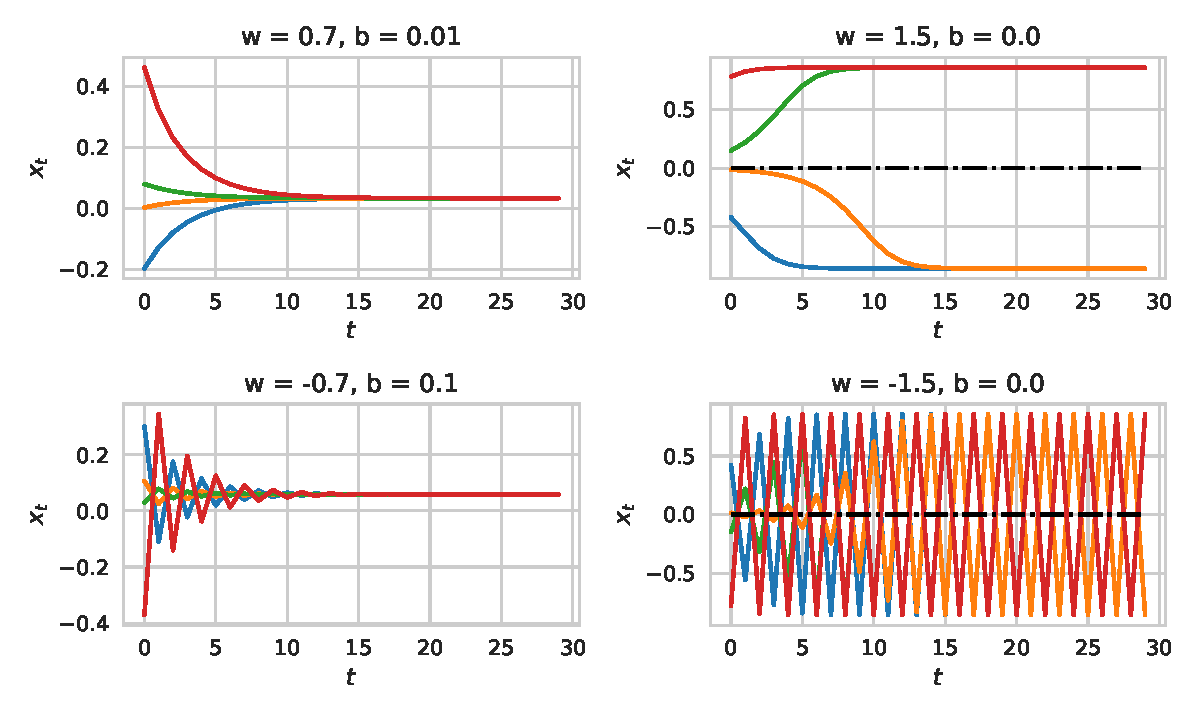
\includegraphics[width=\linewidth]{bif_evolution.pdf}
  \caption{Evolution of $x_t$ over time for different parameters $w$ and $b$.
    Dashed lines show unstable fixed points. Apart from the expected fixed points
    that $x_t$ converges to over time, there are also oscillations visible in
    the last plot. Such oscillations that repeat every 2 iterations are called
    \emph{period-2 cycles} and they appear when $w<-1$.}
  \label{fig:bif_evolution}
\end{figure}
\begin{figure}
  \centering
  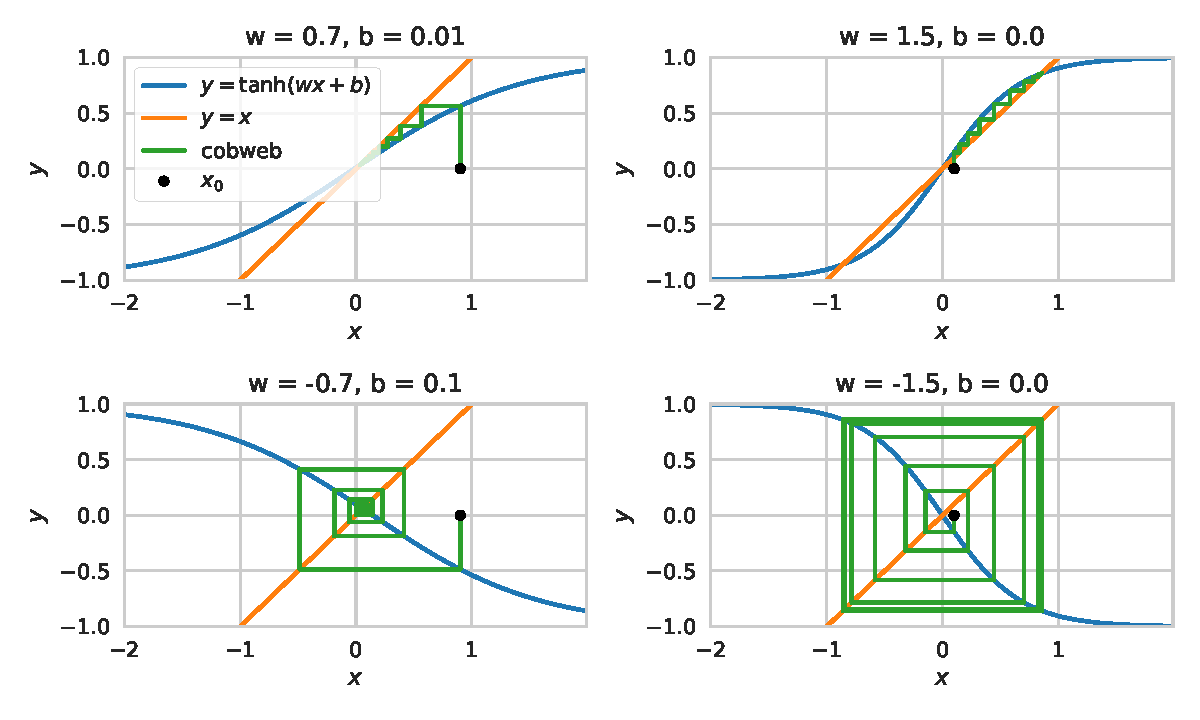
\includegraphics[width=\linewidth]{cobweb.pdf}
  \caption{Cobwebs for the same parameters as in Fig.~\ref{fig:bif_evolution}.
    The black dot is the initial value $x_0$. By drawing a vertical line to the
    intersection with the activation function gives the new input $x_1$. Drawing
    a horizontal line to the intersection with $y = x$ projects the point back to
    the $x$-axis.  The projection is the next input to the activation function.
    This process is repeated until a stable orbit or a fixed point is reached.}
  \label{fig:cobweb}
\end{figure}



By varying the parameters $w$ and $b$ the location and the nature of fixed
points can be changed. The blue line in the right plot of
Fig.~\ref{fig:fixed_points} splits in two as $w$ is increased. The point at
$w=1$ is called a \emph{bifurcation} point.  There are two things that are
happening here: the stable fixed point at $x=0$ becomes unstable (indicated by
the dashed line) and two new stable fixed points above and below zero are
created.

Fixed points can be found analytically by rewriting
Eq.~\ref{eq:single_unit_rnn} with the assumption that $x^*$ is a fixed point
(for which $x_t = x_{t+1}$):
\begin{equation}
  \label{eq:fp}
  x^* = \tanh(wx^* +b).
\end{equation}
Solving once for $w$ and once for $b$ results in two equations for fixed
points:
\begin{align}
  b &= \tanh^{-1}(x^*) - wx^*\\
  w &= \frac{\tanh^{-1}(x^*) - b}{x^*},
\end{align}
which can be plotted for different values of $w$ and $b$
(Fig.~\ref{fig:fixed_points}).  The period-2 cycles cannot be found by
analysing Eq.~\ref{eq:fp}.  Instead they can be found analytically by solving
\begin{equation}
  x^* = \tanh^2(wx^* + b),
\end{equation}
but also by an intuitive, graphical approach called \emph{cobwebbing}
(Fig.~\ref{fig:cobweb}).
Starting from an initial point $x_0$ a vertical line is drawn to the value of
the activation function. Now drawing a horizontal line until we intersect with
the graph of $y = x$ gives the new input $x_1$ and so forth.

\subsubsection{Effect on RNN Training}%
\label{ssub:effect_on_rnn_training}

Now that we have an understanding of what fixed points and bifurcations are we
can examine their effect on RNN learning. Suppose we initialize the network
with a constant $b=0.1$ and a $w=3$. If $x_0$ is negative, the nearest fixed
point is on the lower branch of the yellow line in the right plot of
Fig.~\ref{fig:fixed_points}.  Further assume we train the network to output
$x_\infty = - 0.25$.  In this case, $w$ will be lowered to approach $x^*= -
0.25$ until the bifurcation point is reached and the stable fixed point
vanishes (yellow line becomes dashed line). The fixed point becomes unstable
and the network output will change discontinuously as it jumps to the attractor
on the upper branch.  This will result in a discontinuity in the loss function
and an infinite gradient.  After jumping to the upper branch $w$ will grow
towards infinite values as the GD algorithm tries to approach the target value
of $x = - 0.25$.  Similar examples can be constructed in which parameters
oscillate between two bifurcation points.

The weights of RNNs that are used in practice are normally initialized to very
small values which results
in few fixed points. As the network learns some of the weights increase which
drives the RNN through bifurcations.  The discontinuities that result in very
large gradients cause large jumps of the GD algorithm which can nullify the
learning of hundreds of steps in a single iteration. Aside from the vanishing
and exploding gradient problems, bifurcations are another major reason for the
intricacy of RNN training.

\begin{figure}
  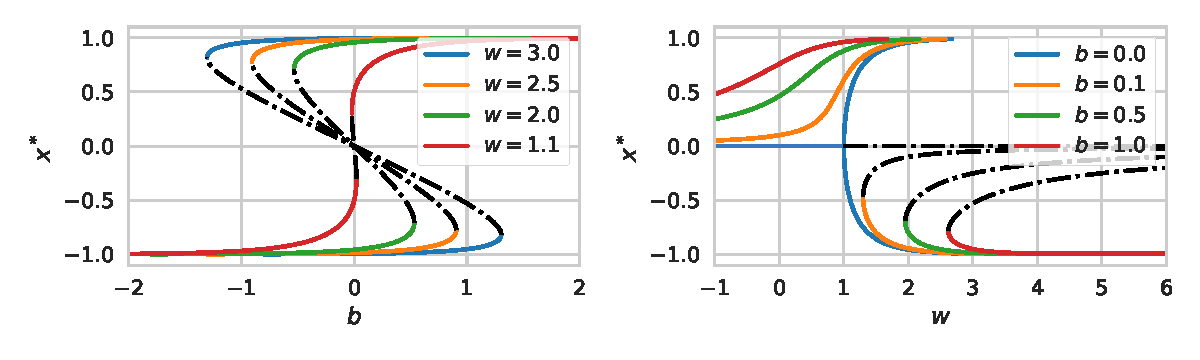
\includegraphics[width=\linewidth]{bif_fixpoints.pdf}
  \caption{Fixed points for different parameter values of $b$ and $w$.  The
    values of the fixed points $x^*$ are affected by varying the weights of the
    RNN.  If there is more than one stable fixed point $x_t$ converges to the
    attractor that is closest to the initial value $x_0$.  Dashed lines denote
    unstable fixed points, which can only be reached if $x_0 = x^*$.}
  \label{fig:fixed_points}
\end{figure}

One solution to all the headaches that are caused by the bifurcations in the
state space, and RNN training in general, is surprisingly simple.  The cause of
bifurcations are adaptions of the recurrent weights of the RNN, so keeping them
constant would eliminate all the complications at once and even come with the
additional advantage of not having to change those weights in the first place.
This might seem like a rather drastic method as the whole ML approach is based on
gradual learning of weights. However, restricting the weight optimization to the
non-recurrent weights frees us from the notorious problems of RNNs and can
perform just as well.  This approach is called \emph{reservoir computing} and
will be discussed in the next Section.

\section{Reservoir Computing}
\label{sec:reservoir_computing}

From the description of the available training methods of RNNs in
Section~\ref{sub:training_recurrent_neural_networks}, one can see that despite
their theoretical capabilities it becomes very difficult to train them in
practice:
\begin{enumerate}
  \item Sequences that require long-range memory are almost impossible to learn,
    due to the vanishing gradient problem of BPTT based optimizers.
  \item The computational complexity of RNN training is very high, with BPTT
    having a complexity of O(n$^2$) per weight update per time step for a
    single output and even O(n$^4$) for RTRL.
  \item Bifurcations in the error surface can prevent the network from
    converging at all.
\end{enumerate}

A recent approach termed \emph{reservoir computing} (RC) that was introduced by
[\cite{lukosevicius}] promises to eliminate almost all the previous
disadvantages by making a conceptual separation between the actual RNN and the
subsequent output layer that maps its internal state to the desired output.
The recurrent part of RNN is regarded as a reservoir, which remains untrained
and only takes the role of mapping the input into a higher dimensional,
temporal representation.  A linear output layer is the only part of the network
that is optimized to produce the desired output from the internal state of the
RNN.

\subsection{Pattern Recognition in a Bucket}%
\label{sub:pattern_recognition_in_a_bucket}

The separation of the recurrent part of the RNN and the output layer is
intuitively described by an experiment called \emph{Pattern recognition in a
bucket} [\cite{Fernando2003PatternRI}], which basically substitutes the RNN with
a bucket of water.  A loudspeaker excites waves on the water surface, which is
filmed and fed into a simple, one-layer feedforward network, equivalent to the
output layer of an RNN.  The output layer is trained on the patterns that arise
from the audio input and a second control network directly on the audio signal.
The control network could not achieve error rates in the classification of
simple words below 25\%, while the networks trained on the water patters made
no more mistakes than 1.5\%.  The reason for this considerable increase in
accuracy is that the water patterns create a high dimensional representation of
the input data.  This representation does not only hold information of the
current time frame, but serves as a memory, as the disturbances in the water
propagate over the whole surface.  Most importantly, this representation is
generated by the underlying physics, which cannot be adjusted to the input
data.  The water has not undergone any kind of training, however, one can still
train the output layer on the deterministically created patterns of its
surface, which nicely illustrates the philosophy of reservoir computing.  The
recurrent weight matrices can, if appropriately initialized, give rise to
similar deterministic patterns in the internal state.


\subsection{The Echo State Network}%
\label{sub:the_echo_state_network}

\begin{figure}
  \centering
  \ESNFlowChart
  \caption{Flow chart of an echo state network. The hatched squares mark the
    untrained weight matrices.}
  \label{fig:esn_flow_chart}
\end{figure}

Mathematically, the part of the static reservoir is taken by the state-space
equation (Eq.~\ref{eq:state_space}) that was introduced in
Sec.~\ref{ssub:state_space_model}.  The weight matrices are initialized during
the setup of the network and are kept static for all times.  Only the weights
of the output layer (Eq.~\ref{eq:readout}) are optimized during the training
phase of the network. This kind of RC network, that is very close to the common
RNN is called \emph{Echo State Network} (ESN). Another kind of RC network is
the \emph{Liquid State Machine}~[\cite{maass2004}], which is studied in
computational neuroscience, as it tries to mimic the spiking neurons of the
brain. It is typically only used for research purposes as its computational
complexity is much higher because it has to compute spiking state activations
in every neuron.

Even though the reservoir is not optimized at all, it still takes the role of a
non-linear expansion into a higher dimensional space and serves as the
short-term memory of the input (Sec.~\ref{sub:short_term_memory}).  This is
possible without adjusting the recurrent weights, given that the initialization
of ESN is done carefully.  In the following we will explore the demands that
need to be made to the reservoir weights in order to ensure its functionality
as a temporal memory, which enables predictions of the future based on the past
inputs.  Assuming that the output layer alone is able to extract the desired
prediction from the current internal state, the ESN should be able to perform
the same tasks as the general RNN. Additionally the problem of bifurcations in
the error surface is eliminated, as the recurrent weights are not altered
during the training. A practical comparison between RNNs and ESNs is hard to do
and no general, objective favorite with regard to performance has been found
yet.


\subsection{The Echo State Property}
\label{sub:echo_state_property}

As the goal of the ESN is to make predictions based on the history of a given
time series, we have to construct an internal state that is a function of the
previously seen inputs, such that
\begin{equation}
  \label{eq:echo_func}
  \vt{x} = f(..., \vec{u}_{t-1}, \vt{u})
\end{equation}
without adjusting the internal weights of the network during training.
An RNN that exhibits this behaviour is said to satisfy the \emph{echo state
property} and called an ESN.  The simplest ESN provides some insight into the
temporal evolution of the internal state. It consists only of one hidden weight
matrix and does not have any external inputs:
\begin{equation}
    \label{eq:state_space_hidden_only}
    \vt{x} = \varphi(\wmatr{} \vec{x}_{t-1})
\end{equation}
By randomly initializing $\wmatr{}$, the only hyper-parameter of the ESN is the
spectral radius $\rho(\wmatr{})$, which is defined as its the largest
eigenvalue:
\begin{equation}
  \rho(\wmatr{}) = \text{max} \{|\lambda_1|, |\lambda_2|, ..., |\lambda_n|\}.
\end{equation}
There exist various libraries that efficiently calculate extremal eigenvalues
for example based on simple power methods (described
in~\ref{sec:spectral_radius}) or more sophisticated methods such as the Lanczos
algorithm~[\cite{lanczos1950iteration}].  Note that the spectral radius scales
with a factor $\alpha$:
\begin{equation}
  \label{eq:spr_scale}
  \rho(\alpha \wmatr{}) = \alpha \rho(\wmatr{}).
\end{equation}
The desired $\rho(\wmatr{})$ can therefore be easily adjusted to an arbitrary
value by multiplying with an appropriate factor.


\begin{figure}
  \centering
  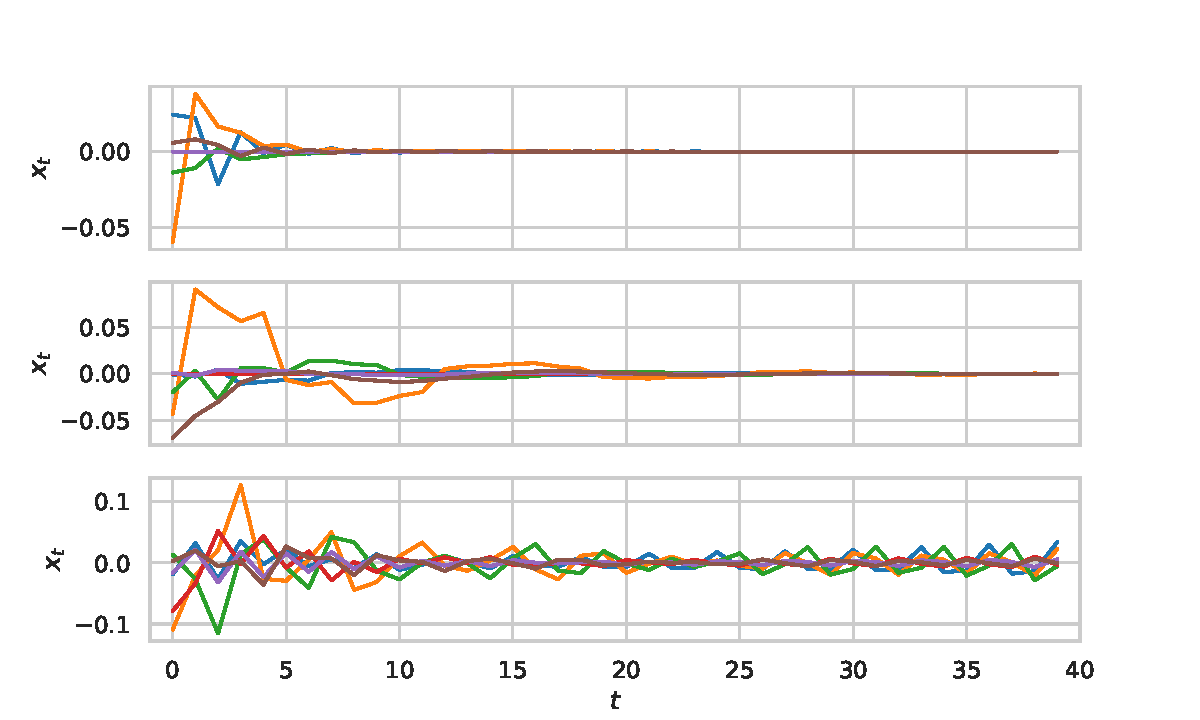
\includegraphics[width=\linewidth]{esn_states_noinput.pdf}
  \caption{State activations of the simple ESN without input weights as defined in
  Eq.~\ref{eq:state_space_hidden_only}. Each line depicts the temporal
  evolution of a single internal state unit. The initial state decays faster in
  the top graph, where the spectral radius is $\rho=0.75$, slower in the middle
  with $\rho=0.95$ and echoes indefinitely in the bottom graph with
  $\rho=1.05$.  The state dynamics are just as expected from the analysis in
  Sec.~\ref{sub:the_bifurcating_state_space}.
  }
  \label{fig:esn_states_noinput}
\end{figure}

As an example we create an initial state $x_0$ randomly from a normal
distribution and the activation function $\varphi$ is taken to be the
hyperbolic tangent.  The smaller the spectral radius, the faster the
information of the initial state should decay as the network is stepping
through time according to Eq.~\ref{eq:state_space_hidden_only}.  The two upper
plots of Fig.~\ref{fig:esn_states_noinput} show exactly this effect.  The first
plot is created by a network with $\rho=0.75$, while the second one is the
result of $\rho=0.95$. The information of the random, initial state
\emph{echoes} much longer with the larger spectral radius and as a result, the
memory of the network becomes longer.  In both cases the echo state property is
satisfied.  In [\cite{jaeger2001}] one can find the formal proof of the
sufficient condition for echo states:
\begin{equation}
  \rho(\wmatr{}) < 1,
\end{equation}
which holds for all monotonically increasing $\varphi$.  In the bottom plot of
Fig.~\ref{fig:esn_states_noinput}, one can see the effect of $\rho=1.05>1$.
Spectral radii $\rho > 1$ would, over time, lead to an exponential growth of
the state activations, if it was not for the bounded, non-linear activation
function $\varphi = \tanh(x)$.  The hyperbolic tangent prevents this divergence
and additionally, the internal state activations never settle down and will go
on echoing forever.  This strongly resembles the periodic fixed points
discussed in Sec.~\ref{sub:the_bifurcating_state_space} and has interesting,
both positive and negative implications for the networks ability to memorize
input and model predictions. Non-linear activation functions such as the
hyperbolic tangent often prevent the state from exploding, thus making it
possible to use spectral radii larger than one. This can still yield valid echo
states, but the risk of over-saturating the state becomes much higher.  This
saturation is caused by the internal dynamic that is introduced to the state by
entering the non-linear regime of the activation function and the resulting
periodic fixed points.  If the internal dynamic starts dominating the input to
the ESN it becomes useless, as all the external information is overwritten by
its internal dynamics.  The implications that a varying spectral radius has for
the performance of the ESN on different datasets is discussed in
Chapter~\ref{cha:results}.\\


\subsection{Reservoir With Inputs}
\label{sub:reservoir_without_feedback_weights}

In the more practical case of an ESN with external inputs, the internal state
and thus the memory of the network is also influenced by the degree of which
the input overwrites the previous internal state.  To incorporate a scalar
input in the network we introduce an input weight matrix $\wmatr{in}$ with
dimensions $(N \times 1)$.
\begin{equation}
  \label{eq:state_space_no_feedback}
  \vt{x} = \varphi(\wmatr{in}  \vt{u} + \wmatr{hidden} \vec{x}_{t-1}).
\end{equation}

The range of values that $\wmatr{in}$ is initialized with is a typical
hyper-parameter for which there are no solid guidelines, apart from choosing
small values.  We will choose a uniform distribution of values between $-\kappa
< 0 < \kappa$, where $\kappa$ is typically smaller than one half. The
implications of different initializations are shown in
Fig.~\ref{fig:esn_states_input}.  It shows how the internal state reacts to a
scalar input in form of a simple step function. 

For a small $\rho=0.5$ and large $\kappa=0.1$, the state $x$ is dominated by
the input, which is visualized in Fig.~\ref{fig:esn_states_input} B.  The state
activations quickly approach a certain value and form a plateau after just three
to four time steps. When such a plateau is reached in all state activations,
the network cannot determine the current position in the time series any more
and will loose its predictive power.  In plot C the network is set up with
$\rho=0.9$ and $\kappa=0.02$.  It takes longer for the initial random state to
decay and the individual activations are not reaching a plateau any more.  From
the recurring state activations that are the same after each period but
different for each point within one period, the network can infer where in the
time series it currently is and make an accurate prediction for the next step.
\begin{figure}
  \centering
  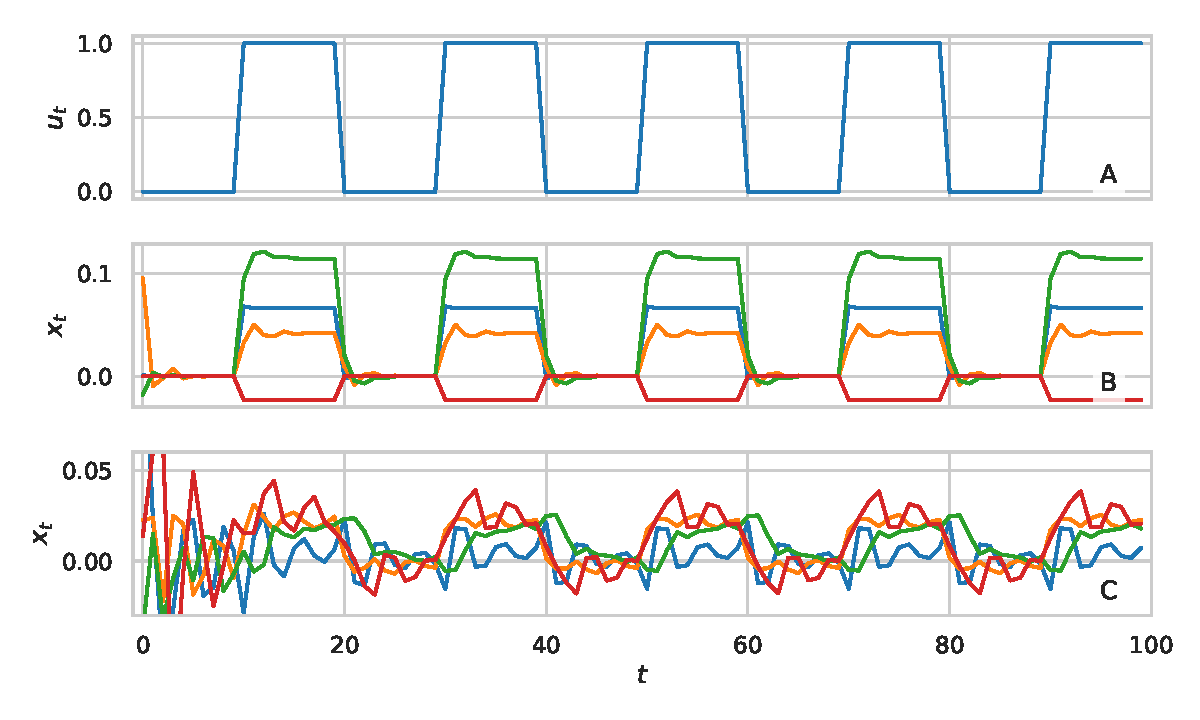
\includegraphics[width=\linewidth]{esn_states_input.pdf}
  \caption{Reaction of the internal state of the ESN to external input $u(t)$
  (step function in graph A).
  A large $\kappa$ leads to the input dominating the internal state, while a
  smaller $\kappa$ enables it to memorize previous inputs.}
  \label{fig:esn_states_input}
\end{figure}

Both $\rho$ and $\kappa$ must be chosen with respect to the task at hand.  The
last hyper-parameter of the ESN is the sparsity of the reservoir matrix
$\wmatr{}$. It only affects ESN memory for values well above 95\%
[\cite{farkavs2016}], but it can significantly reduce computational complexity
for large reservoir sizes.  The specific choice of these parameters can be made
with a hyper-parameter optimizer, as described in
Sec.~\ref{sec:hyper_parameter_optimization}.


\subsection{Short-term Memory \& Reservoir Non-linearity}%
\label{sub:short_term_memory}

Short-term memory describes the dynamic memory of an internal ESN (or more
generally RNN) state, which should not be confused with the memory of a network
that is brought about by weight adaptions (e.g. through gradient descent),
which is called long-term memory.  We have already convinced ourselves that the
internal state acts as a memory of the previous inputs, as depicted in
Fig.~\ref{fig:esn_states_noinput}.  This memory could be almost arbitrarily
long if it were not for the problem of vanishing gradients of very deep
networks, which bounds the length of a practically learnable sequence to a
number of data points in the order of ten.  As already discussed, ESNs avoid
the vanishing gradient problem altogether by not calculating recurrent
gradients at all. Without this problem, how much can an ESN remember?  It was
shown by [\cite{jaeger2002}] that for linear recurrent weights (where the
activation function is the identity) the \emph{memory capacity} (MC) is equal
to the size of the ESN state:
\begin{equation}
  \text{MC} = N_{units} \text{ .}
\end{equation}

The memory capacity is defined as the number of inputs that a perfectly trained
output matrix $\wmatr{out}$ can extract from an ESN state which was created by
feeding it a random sequence.  A random sequence in this context means a series
of numbers that were drawn from a uniform distribution. How to practically measure
MC is shown in Sec.~\ref{sec:short_term_memory}. Essentially the value of the MC
gives a measure of how many input steps the ESN can encode in its internal state.

For the case of a non-linear activation function in the recurrency of the ESN
the MC has an upper bound:
\begin{equation}
  \text{MC} < N_{units} \text{ .}
\end{equation}

Intuitively one might think that a larger MC will
automatically lead to a better performing prediction. However, there is a
second requirement that needs to be fulfilled in order to predict chaotic
systems well: The degree of non-linearity (essentially expressed by the
spectral radius) of the reservoir must be appropriate for the task.
A network with the hyperbolic tangent as an activation function and 
a spectral radius close to or smaller than one acts mostly in the
linear regime of the tanh. This means that the dynamics of the internal state
are governed by an approximately linear expansion and in turn makes it very
hard for the (also linear) output layer to produce a chaotic prediction.
The obvious solution is to increase the spectral radius to values greater than
one, but it turns out that there is a tradeoff between MC and the non-linearity
of the ESN reservoir. Increasing the spectral radius above one degrades the
memory of the ESN (Sec.~\ref{sec:short_term_memory}), but makes it possible
to predict chaotic systems (Sec.~\ref{sec:res_mackey_glass_system}).
A potential solution to this problem lies in separating the memory of the ESN
from is linear transformation. This was attempted with an extension of the ESN
to R$^2$SP (random static projections) by [\cite{butcher2013}], but its treatment
is out of the scope of this work.


\subsection{ESN Training}
\label{sub:esn_training}

To train an ESN any of the previously introduced methods for training RNNs can
be used. The fact that only the last layer is trained makes an additional, much
faster least squares method possible.  In the case of a linear output layer,
the predictions of the network can be written as
\begin{equation}
  \vt{y} = \wmatr{out} \vt{x},
  \label{eq:esn_lin_out}
\end{equation}
where $\vt{x}$ can generally either be the internal state or the internal state
concatenated with the corresponding input $\vt{u}$.  By collecting a number of
states (and inputs) that are created with the untrained network, we can rewrite
Eq.~\ref{eq:esn_lin_out} into Eq.~\ref{eq:esn_lin_out_concat} with concatenated
states $\matr{X}$ and desired outputs $\matr{D}$.
\begin{align}
  \matr{X} &:= (\vec{x}_1, ..., \vec{x}_T) \\
  \matr{D} &:= (\vec{d}_1, ..., \vec{d}_T) \\
  \matr{D} &= \wmatr{out} \matr{X} \label{eq:esn_lin_out_concat}
\end{align}

To find the optimal weights $\wmatr{out}$ we have to solve the overdetermined
system in Eq.~\ref{eq:esn_lin_out_concat}, which can be done for example via
the pseudo-inverse method.  It even gets by without introducing an
additional hyper-parameter by utilizing the Moore-Penrose pseudo-inverse
$\matr{X}^+$:

\begin{align}
  \wmatr{out} &= \matr{D}\matr{X}^+ \\
  \matr{X}^+  &= (\matr{X}^T\matr{X})^{-1} \matr{X}^T
\end{align}



Another method is called \emph{Tikhonov Regularization}, which, outside
geophysical contexts, is more frequently called \emph{ridge
regression}~[\cite{MontgomeryRegression}]:
\begin{equation}
  \label{eq:tikhonov}
  \wmatr{out} = \matr{D} \XT (\matr{X} \XT - \beta \matr{I})^{-1}
\end{equation}
The regularization coefficient $\beta$ is introduced to reduce the risk of
overfitting the output weights, which will quickly lead to diverging
predictions when feeding the output of the ESN back into the input.
Effectively $\beta$ becomes another hyper-parameter, which has to be tuned in
order to obtain good results.  A derivation of Tikhonov Regularization can be
found in the Appendix~\ref{sec:tikhonov_regularization}.  

\section{Hyper-parameter Optimization}%
\label{sec:hyper_parameter_optimization}

Before a machine learning model can be trained, certain decisions regarding the
architecture of the network have to be made. This involves parameters such as
the number of layers in feedforward networks, kernel sizes in
convolutional nets or, as in the case of the ESN, sparsity and spectral radius
of the reservoir.  These parameters are called \emph{hyper-parameters} (HP) and
they fill a compact space $\mathbf{X}$.  The goal of HP optimization is to find
a configuration $\mathbf{x_i}$ that maximizes the performance of the network:
\begin{equation}
  \arg \max_{\mathbf{x_i} \in \mathbf{X}} f(\mathbf{x_i})
\end{equation}
The function $f$ is not known and very expensive to evaluate as one evaluation
amounts to the creation of a trained NN.  Often this optimization problem is
solved by handily tuning each HP until a \emph{reasonably} good
$\mathbf{x_{\text{opt}}}$ is found, but there are a few methods that can be
applied to automate this process.  The two simplest methods are \emph{grid
searches} and \emph{random searches} of the HP space.  First, the space of
valid HPs is defined.  For example, a number of units $N = (10, 20, 30,...,
100)$ and a learning rate $\eta = (0.1, 0.01, 0.001, ...)$. Grid search then
performs an exhaustive search of all parameters, which is very simple to
implement but suffers from the curse of dimensionality.  Random search randomly
samples $\mathbf{x_i}$ from the HP space, which does not have the problem of
needing to perform an exhaustive search and is widely applied in practice, as
it is still very simple to implement.

The next section describes an algorithm called \emph{Bayesian Optimization},
which also samples the next $\mathbf{x_i}$ but incorporates the knowledge of
already evaluated points in the HP space.  It utilizes Bayes' Theorem which,
adjusted to this problem, states that the \emph{posterior} probability
distribution of a model $M$ (over the HP space $\mathbf{X}$) given a number of
already evaluated samples $A \in \mathbf{X}$ is:
\begin{equation}
  P(M|A) \propto P(A|M) P(M),
\end{equation}
where $P(M)$ is the \emph{prior} probability distribution over $X$, and
$P(A|M)$ the \emph{likelihood} of the samples given $M$.


\subsection{Bayesian Optimization}%

The following description is largely based on article~[\cite{brochu2010bayesopt}]
and will briefly introduce the concept of Gaussian
Processes and how they are used in Bayesian Optimization as introduced
by~[\cite{williams1996gaussian}].  In summary, the Bayesian Optimization
algorithm tries to maximize an objective function $f$ by balancing exploration
(evaluating areas where the true values of $f$ are very uncertain) and
exploitation (which tries to evaluate $f$ where it is expected to be high). It
rests upon the concept of Gaussian Processes (GP), which can be used to define
a distribution over $f$.  From the GP it is possible to calculate an
acquisition function, which is used to efficiently sample the next
$\mathbf{x}_i$ that should be evaluated.  There are different acquisition
functions that emphasize either exploration or exploitation. The method of
Bayesian Optimization yields good results with only few evaluations and is very
likely to perform well on objective functions with local maxima.\\

\subsubsection{Gaussian Processes}%
\label{ssub:gaussian_processes}

A GP is defined by its mean function $m(\mathbf{x}_i)$ and its covariance
function $k(\mathbf{x}_i, \mathbf{x}_j)$.  This means that to each argument
$\mathbf{x}_i$ we assign a random variable $f(\mathbf{x}_i)$.  In analogy to
the Normal distribution, a GP is formally written as:
\begin{equation}
  f \sim {GP}(m,k)
\end{equation}
where $m(\mathbf{x}_i)$ can be any function but typically is just zero, and a
common covariance matrix is created with a Gaussian kernel:
\begin{equation} \label{eq:cov}
  \mathbf{K}_{ij} = k(\mathbf{x}_i, \mathbf{x}_j) =
      \exp \bigg(\frac{- ||\mathbf{x}_i - \mathbf{x}_j||^2}{2}\bigg).
\end{equation}
This kernel is close to one for values close to each other and approaches zero
as the values grow further apart, which implies that close values are highly
correlated.
With this definition, a GP is equivalent to a multivariate Gaussian
$\mathcal{N}(\mu, \Sigma)$ with mean vector $\mu$ and a covariance matrix
$\Sigma$:
\begin{align}
  \mu_i &= m(\mathbf{x}_i) \\
  \Sigma_{ij} &= k(\mathbf{x}_i, \mathbf{x}_j)
\end{align}

Given mean and covariance we can use the GP as a prior for the function $f$ of
which we want to find the maximum. By choosing a zero mean, the only actual
prior information is a smoothly operating $f$, implied by the Gaussian kernel.
The interesting part is how to update this prior with information that is
gained by evaluating $f$ a certain point to obtain a posterior.  Assuming that
we already have $n$ observations $\{\mathbf{x}_{1:n} ; f(\mathbf{x}_{1:n})\}$
we can find the covariance matrix $\mathbf{K}$ with Eq.~\ref{eq:cov}.  To find
the probability distribution of an unobserved point $\mathbf{x}_{n+1}$, the
conditional probability of $f_{n+1}$ given the previous observations (also
called predictive distribution) is needed:
\begin{equation}
  P(f_{n+1} | \mathbf{x}_{1:n} ; f(\mathbf{x}_{1:n})) 
    = \mathcal{N}(\mu_p(\mathbf{x}_{n+1}) , \sigma_p^2(\mathbf{x}_{n+1})),
\end{equation}

where $\mu_p$ and $\sigma_p$ are the predicted mean and standard deviation at
an unknown point.  They can be calculated thanks to the properties of the GP,
which state that the observations and the arbitrary point $\mathbf{x}_{n+1}$
are jointly Gaussian:
\begin{align}
  &\begin{bmatrix} f(\mathbf{x}_{1:n}) \\ f(\mathbf{x}_{n+1}) \end{bmatrix}
  \sim \mathcal{N} \bigg(
    0,  \begin{bmatrix} 
           \mathbf{K} & \mathbf{k}^T \\ 
           \mathbf{k} & k(\mathbf{x}_{n+1}, \mathbf{x}_{n+1})
        \end{bmatrix}
  \bigg) \\
  &\mathbf{k} = \begin{bmatrix}
      k(\mathbf{x}_1, \mathbf{x}_{n+1}) &
      \dots &
      k(\mathbf{x}_n, \mathbf{x}_{n+1})
  \end{bmatrix}
\end{align}

From this it is possible to derive that:
\begin{align}
  \mu_p (\mathbf{x}_{n+1}) &= \mathbf{k}^T \mathbf{K}^{-1} f(\mathbf{x}_{1:n}) \\
  \sigma_p (\mathbf{x}_{n+1}) &= k(\mathbf{x}_{n+1}, \mathbf{x}_{n+1}) 
                               - \mathbf{k}^T \mathbf{K}^{-1} \mathbf{k}
\end{align}

The resulting predictive distribution is typically very cheap to evaluate as
the number of observations is low. With this distribution it is possible
to find the so called \emph{acquisition function}, which enables an educated
guess of the next best point of evaluation of the objective function.

\label{sub:bayesian_optimization}
\begin{figure}
  \centering
  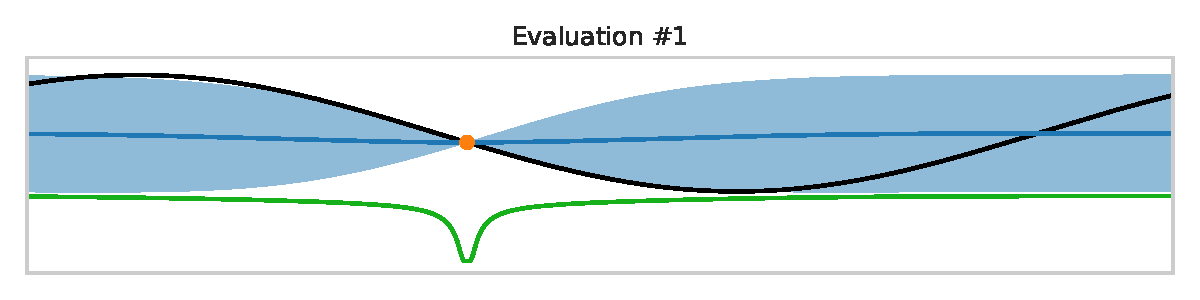
\includegraphics[width=\linewidth]{gpopt_01.pdf}
  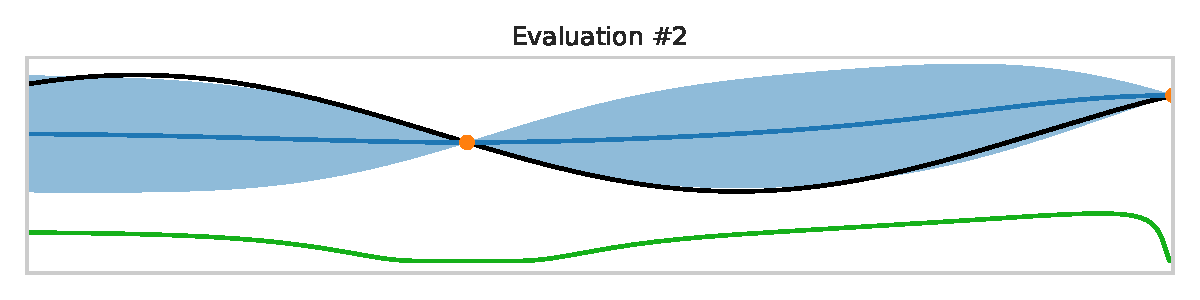
\includegraphics[width=\linewidth]{gpopt_02.pdf}
  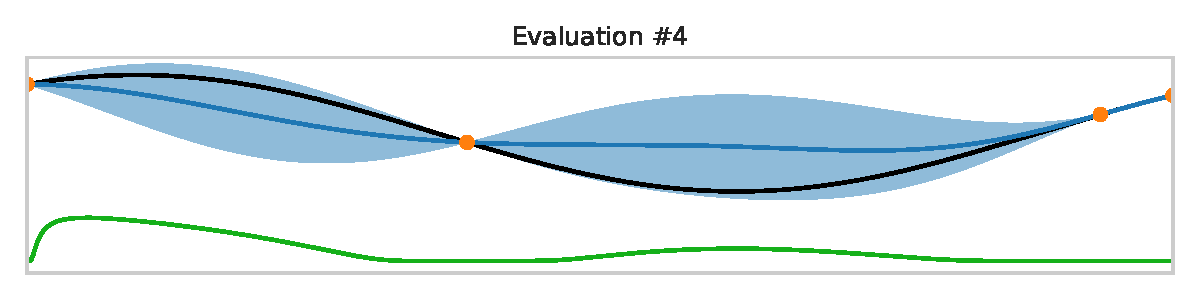
\includegraphics[width=\linewidth]{gpopt_04.pdf}
  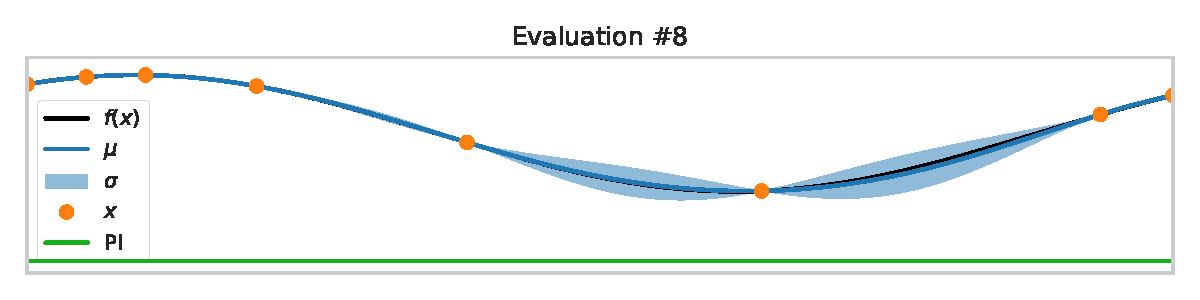
\includegraphics[width=\linewidth]{gpopt_08.pdf}
  \caption{A timeline of Bayesian Optimization. The plots show how the GP
    approximates the objective function better and better after each iteration.
    The maximum of the green acquisition function indicates where $f$ will be
    sampled next.  The uncertainty of already observed points is zero in this
    case, as there is no noise incorporated in the example. However, noisy
    objective functions can be dealt with by only slight additions to the
    described algorithm. An in depth description of Gaussian Processes and
    how they can be applied to ML can be found in~[\cite{rasmussen2004gaussian}].
  }
  \label{fig:gpopt_01}
\end{figure}


\subsubsection{Acquisition function}%
\label{ssub:acquisition_function}

The acquisition function is obtained from the predictive distribution of the 
GP and is defined such that it is high where the objective function $f$ is
\emph{potentially} high.  The probability of large objective values is high
where either the uncertainty or the mean (or both) of the GP are large. 
Maximizing the acquisition function amounts to sampling $f$ at
\begin{equation}
  \mathbf{x}_{n+1} = \arg \max_{\mathbf{x_i} \in \mathbf{X}} 
                     \text{ PI}(\mathbf{x}_i).
\end{equation}
The function PI is an example of an acquisition function called the
\emph{probability of improvement}:
\begin{align}
  \text{PI}(\mathbf{x}_i) &= P(f(\mathbf{x}_i) > f(\mathbf{x}^+)) \\
  &= \Phi\bigg( \frac{\mu_p(\mathbf{x}_i) - \mu_p(\mathbf{x}^+)}
                     {\sigma_p(\mathbf{x}_i)}  \bigg) \nonumber
\end{align}
Here $\Phi$ is the cumulative distribution function. The emphasis of PI clearly
lies on exploitation, as samples with a mean lower than the current maximal
mean will never reach PI values over 0.5.  More sophisticated acquisition
functions than PI, which are not purely driven by exploitation include
\emph{expected improvement}. A description of various acquisition functions
and Bayesian Optimization as a whole can be found in~[\cite{brochu2010bayesopt}].

\chapter{Implementation}
\label{cha:implementation}
\epigraph{
  This chapter provides an overview over the problem we are trying to solve
  and shows how it was translated into a Tensorflow model.
  It highlights the most important technical considerations
  that were made during the implementation of the anomaly detection,
  which was described theoretically in the previous chapters. The different
  parts of the model, from input pipeline, over the ESN architecture to the
  hyper-parameter and weight optimizations, are illustrated with some brief
  pseudocode snippets.
}


\section{Development}%
\label{sec:development}

The code for this thesis was written in Numpy, Scipy, and Tensorflow, and
is implemented as a Python package named \ttt{torsk}.
Tensorflow [\cite{tensorflow2016}] is the most commonly used framework for
implementing ML models. It is an open source library that is maintained mostly
by Google engineers. In addition to implementing the most common GD algorithms,
from plain GD to more advanced algorithms such as Adam, Tensorflow takes care
of parallelizing and distributing the large matrix operations that make ML so
powerful.  The core design principle of Tensorflow is to separate the build and
execution phases of the model. First, the desired model architecture is
constructed by defining the \emph{computational graph}. This graph is then
optimized and during model execution certain nodes in the graph can be
requested for evaluation.  Tensorflow will then only execute the parts of the
model that are necessary to evaluate the requested node. Some of the more
intricate solutions that are presented (especially in
Sec.~\ref{sec:encoder_decoder}) might be obsolete by the time of reading, as
Tensorflow was under heavy development. It had not reached a stable API during
the main development phase of the code, which was written mainly in Tensorflow
versions 1.6-1.9.


\subsection{The Journey}%
\label{sub:the_journey}
The implementation of the algorithm that was described theoretically in the
previous chapters is the result of a search for a suitable RNN architecture and
training method that has required numerous trial and error attempts.  The
result is a carefully orchestrated model that allows the prediction of
high-dimensional, spatio-temporal, chaotic systems. Although it should be quite
straight forward to implement a functioning ESN, with the theoretical
background that was laid in the two previous chapters, the model is quite
easy to break. Slightly defective training procedures can lead to the
reproduction of the current time frame instead of a prediction of the future.
Once the network is correctly implemented, it still is not trivial to make it
produce sensible predictions for different datasets due to the large number of
hyper-parameters that have to be set.  Erroneous hyper-parameter setups easily
result in predictions that quickly diverge, or do nothing but decay to the mean
value of the input sequence.  Especially the last error is very hard to fix
without a good intuition of the internal dynamics of the ESN.  Tensorflow's
rather opaque RNN programming model does its part in slowing down the
resolution of these problems.

At the beginning of this thesis it was not yet clear that the final approach
would involve reservoir computing, which does not need to make use of the very
convenient gradient and automated differentiation methods that Tensorflow
offers. However, the automatic parallelization of the network still comes in
handy. Additionally, Tensorflow comes with a tool called TensorBoard, which
makes it easy to visualize the network architecture
(Fig.~\ref{fig:network_graph}) and the learning performance during development.
A reevaluation of the advantages and drawbacks of Tensorflow and a second ML
framework called \emph{PyTorch}, that is currently gaining popularity, would
most probably lead to the choice of PyTorch over Tensorflow.  The dynamic
features that are needed to implement RNNs are accesible in a much more
pythonic way in PyTorch. Additionally, PyTorch seems to be faster at RNN tasks
than Tensorflow, but this claim was not veryfied personally. That being said,
PyTorch is still in an even earlier stage of development than Tensorflow, and
was not as popular in the beginning of this work.


\section{The \texttt{torsk} Python Package}%
\label{sec:torsk}

The code that was developed in this work can be found on GitHub
[\cite{coderepo}], code snippets that are presented here are partially simplified
to pseudocode to highlight only the important parts of the implementation and
reduce the amount of cited boilerplate code. The parts where this is done are
recognizable through inline comments.

The package that implements the anomaly detection is subdivided into three main
parts: \ttt{torsk.datasets} (containing functions that create input pipelines
for the different datasets), \ttt{torsk.esn} (where the ESN implementation
itself is located), and \ttt{torsk.models} (containing different network
architectures). The two most important models are the \ttt{grad} model,
implementing the prediction with Tensorflow optimizers and the \ttt{lms} model,
which uses Least Mean Squares techniques, such as Tikhonov Regularization.  In
addition, there are two small visualization and analysis submodules to inspect
the output of the Tensorflow models.

\begin{figure}
  \centering
  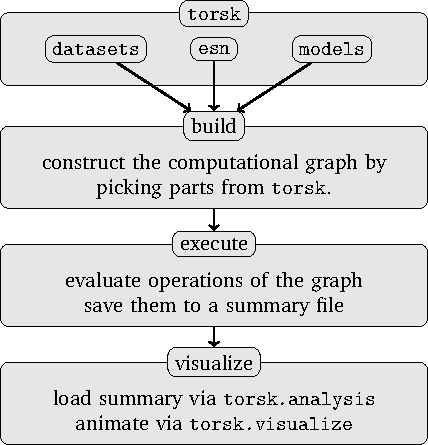
\includegraphics[width=0.5\linewidth]{tikz/flow.pdf}
  \caption{Flow chart of the execution of \texttt{torsk} as it is realized with
  its run scripts. The top node is mean to illustrate which components of the
  package are needed to build a prediction network.}
  \label{fig:flowchart}
\end{figure}

Fig.~\ref{fig:flowchart} shows a flow chart of the anomaly detection
execution, to provide an overview over how it works.  To realize the
anomaly detection in Tensorflow, it is broken down into three phases: First,
the build phase, where the computational graph is constructed. Second, the
execution phase, which evaluates the graph in an appropriate order to optimize
the ESN and make predictions. And third, the visualization of the results.  If
an online learning model (powered by GD algorithms) is run, then the execution
and visualization phases can also be unified.

Once the graph is constructed it is easy to pick out the operations
that are desired and evaluate them using Tensorflow primitives. As the
execution and visualization phases of the algorithm are rather straight forward
and can be examined more closely in the examples of the \ttt{torsk} repo, the
rest of this section will focus on the build phase of the network. 


\section{Building The Computational Graph}%
\label{sec:building_the_computational_graph}

Before getting into the concrete implementation details of the graph, let us
restate what we are trying to achieve:  Based on an input sequence $\mathbf{u}$
we want to create a prediction $\mathbf{y}$ and compare this prediction to the
truth $\mathbf{d}$ so that we can identify an anomaly based on the deviation of
$\mathbf{y}$ and $\mathbf{d}$. 

This problem can be broken down in a few steps to gradually build up the
complete computational graph (Fig.~\ref{fig:network_graph}), which are listed
below.  Reminder: A frame of the input sequence $\mathbf{u}$ at time $t$ is
denoted by $\vt{u}$ (analogous for $\mathbf{y}$ and $\mathbf{d}$).

\begin{figure}
  \centering
  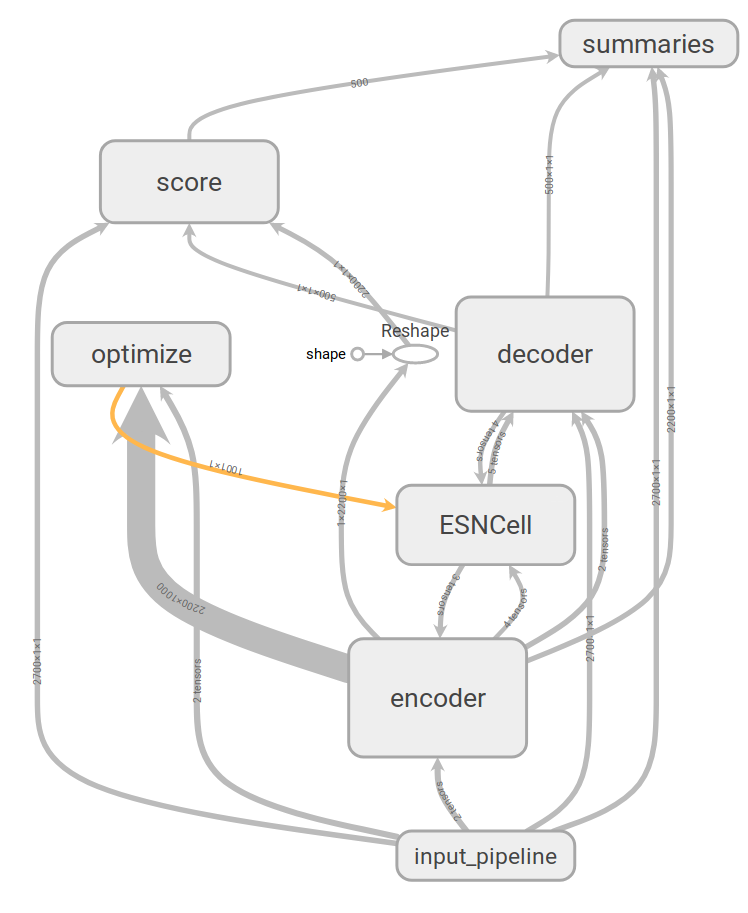
\includegraphics[width=0.8\linewidth]{network_graph.png}
  \caption{Network graph as created by TensorBoard. The nodes represent the
  tensors that hold the actual values of input frames, weight matrices, etc.
  The edges represent the operations, such as multiplications/additions, which
  specify the data flow through the graph. The specified operations are evaluated
  during the execution phase of the network within a \ttt{tf.Session}.}
  \label{fig:network_graph}
\end{figure}


\begin{enumerate}
  \item \textbf{Read} the input sequence $\mathbf{u}$. Implementation described
    in (Sec.~\ref{sec:input_pipeline}) and represented by the \emph{input
    pipeline} node in the network graph. The input pipelines are defined in
    \ttt{torsk.datasets} and essentially convert Numpy arrays into Tensorflow's
    tensors.

  \item \textbf{Feed} the input sequence $\mathbf{u}$ to the ESN. The ESN cell
    itself, with all its weights is represented by the \emph{ESNCell} node. The
    \emph{encoder} node takes care of looping over the input and feeding it
    frame by frame to the ESN, as well as recording the created internal states
    $\vt{x}$ and ESN outputs $\vt{y}$.

  \item \textbf{Train} the ESN. This is done by the \emph{optimizer} node, which adjusts
    the output weights of the ESN such that the outputs $\vt{y}$ match
    $\vec{u}_{t+1}$ as closely as possible.

  \item \textbf{Predict} the sequence $\mathbf{y}$.  Similarly to step two the
    \emph{decoder} feeds the necessary data to the ESN.  The only difference is
    that now the output of the cell is fed back to its input. This node implements
    the \emph{freely running} ESN.

  \item \textbf{Detect} the eventual anomalies based on $\mathbf{y}$ and
    $\mathbf{d}$.  Described in Sec.~\ref{sec:anomaly_detection_model} and
    represented by the \emph{score} node. The sliding score is implemented both
    in Tensorflow and Numpy in \ttt{torsk.score}.

  \item Evaluate the detected anomalies. This requires human interaction.
\end{enumerate}

The steps 2.-4. are implemented in the \ttt{torsk.models} submodule and
represent most of the logic of the network and the ESN implementations
themselves reside in \ttt{torsk.esn}.  In the following sections we will
revisit the main nodes of the network to describe some specific implementation
details that are worth noting.



\subsection{Input Pipeline}%
\label{sec:input_pipeline}
\begin{listing}
  \inputminted{py}{pseudocode/input_pipeline.py}
  \caption{Simplified input pipeline for sea surface height (SSH) data. The
  lower part of the snippet shows the build phase of a very simple graph and
  how it is executed within a \texttt{tf.Session}.}
  \label{lst:pipeline}
\end{listing}


The goal of the input pipeline is to create an \ttt{inputs} and a \ttt{labels}
sequence that represent the series of inputs $\vt{u}$ and the desired outputs
$\vt{d}$.  The input pipeline takes care of reading slices of the input
sequence to disk and hands them over to the parts of the NN architecture where
it is needed.  There are several ways of doing this in Tensorflow, but the
recommended one is to use the \emph{Dataset API} (\ttt{tf.data.Dataset}).  If
the data is not stored in the TFRecord format a dataset can be created from a
Python generator.  In the case of climate model output they are typically
NetCDF files.  The generator reads in the data, normalizes the values, and
yields time slices of a desired length (Lst.~\ref{lst:pipeline}).  The
generator is now converted into a dataset, which calls the generator as often
as necessary to apply the defined transformations.  The only significant
operation that is applied to the SSH images is resampling them to a desired
size.  To comply with the Tensorflow \emph{Estimator API} the pipeline returns
a dictionary of all features and a single Tensor of labels.  The current input
pipeline is a very simple implementation that was not optimized with regard
to speed, as this was not a bottleneck yet. It might have been sufficient to
just work with \ttt{tf.placeholder} constructs instead.  But because the final
goal was to create an automated detection algorithm that can skim through a lot
of data it seemed feasible to start using the slightly more complicated Dataset
API. In addition, the input functions that are created with the Dataset API can
be used in conjunction with the Estimator API.


\subsection{Echo State Network Cell}%
\label{sec:echo_state_network_cell}

\begin{listing}
  \inputminted{py}{pseudocode/esn_cell.py}
  \caption{Pseudo code for the densely represented ESN cell. The full
  implementation is located at \ttt{torsk.esn.esn\_cell}.}
  \label{lst:esn_cell}
\end{listing}

The central part of the anomaly detection algorithm is the ESN cell, as
governed by the state space equations, which were introduced in
Sec.~\ref{ssub:state_space_model}. It is implemented both in a dense
representation in the \ttt{ESNCell} and a sparse respresentation in the
\ttt{SparseESNCell}.  To create an RNN in Tensoflow's computational graph, it
has to be unrolled along the time axis. For standard RNN tasks the graph
creation is conveniently handled by the \ttt{tf.nn.dynamic\_rnn} function,
which only needs a \ttt{tf.nn.rnn\_cell.RNNCell} object and some inputs to
work.  The ESN cell is implemented as a subclass of the
\ttt{tf.contrib.rnn.LayerRNNCell}, which in turn is a subclass of the RNNCells
to make them act like proper \ttt{tf.Layer} objects.  An RNNCell needs to
implement the \ttt{state\_size} and \ttt{output\_size} properties, as well as a
\ttt{build} and a \ttt{call} method.  The build method initializes all the
weights that are needed in the call method, which defines the operations that are
executed at each time step of the RNN.  In most Tensorflow RNN cells the output
weights are defined outside the cell class as they are not part of the
recurrency. The reasons for including them, as well as the state variable that
is returned twice by the call method, will become clear during the section on
the encoder and decoder of the network (Sec.~\ref{sec:encoder_decoder}).
Pseudo code for the ESNCell is given in Lst.~\ref{lst:esn_cell}.

The initialization of the ESN reservoir is done via a custom
\ttt{ESNReservoirIntitializer}.  It inherits from the standard Tensorflow
\ttt{Initializer} class and essentially calls a function that creates a
reservoir matrix in Numpy and converts it to a \ttt{tf.Tensor}.


\subsection{Encoder \& Decoder}%
\label{sec:encoder_decoder}

\begin{listing}[t]
  \inputminted{py}{pseudocode/build_model.py}
  \caption{Functions that create the prediction helper and decoder to feed the
  output of the ESN back to the input.}
  \label{lst:decoder}
\end{listing}

The encoders and decoders of an RNN take over the task of feeding the right
inputs to the network during the training (encoder) and prediction (decoder)
phases. The names encoder and decoder stem from the primary application of RNNs to
natural language processing tasks.  In language processing every word needs to
be encoded into a (typically binary) vector representation before it can be fed
to the network, hence the name. In our case the only thing the encoder does is
to feed the true input $\vt{u}$ to the network and to record the corresponding
output $\vt{y}$ for every frame in the input sequence. This is normally done by
the \ttt{tf.nn.dynamic\_rnn} function.  The decoder is used during the
prediction phase of the network.  It takes care of feeding the current
prediction $\vt{y}$ back to the ESN as the next input $\vec{u}_{t+1}$, which is
not possible with the dynamic RNN encoder.  Instead, the
\ttt{tf.contrib.seq2seq.dynamic\_decode} (line 35 of Lst.~\ref{lst:decoder})
routine can be used. It unrolls the ESN based on a decoder object, which in
turn needs a helper to define the next inputs and the state of the ESN.
Unfortunately, the \ttt{dynamic\_decode} function only returns, apart from
the prediction, the final state of the ESN and none of the intermediate states.
This is a major inconvenience for ESN debugging, which is why the custom ESN
cells (Sec.~\ref{sec:echo_state_network_cell}) return the state variable twice.
This way they are treated like outputs, collected at every step, and
returned together with the cell outputs in the end.  Unfortunately, the
practical realization of this idea is a slightly tedious task in Tensorflow
that includes creating a custom \emph{helper}, which, at the time of writing,
are rather sparsely documented.  However, it can be done as shown in
Lst.~\ref{lst:decoder}. The \ttt{prediction\_helper} function defines three
functions that are needed to create a custom helper, which define the behaviour
of the helper during the unroll of the ESN.  Custom helpers provide quite some
flexibility, including sampling next inputs from either labels (desired
outputs) or predicted outputs, but this is not needed here, so \ttt{sample\_fn}
just returns an arbitrary value.  The \ttt{next\_inputs\_fn} function is called
at each prediction step with the previous cell output as one of its input
arguments.  The important thing is that on line 20 of Lst.~\ref{lst:decoder}
only the current prediction $\vt{y}$ is picked as the next input.
Unfortunately, the extraction of all the intermediate states from the decoder
involves changing the return statement of the ESN cells, which breaks them for
the usage with \ttt{tf.nn.dynamic\_rnn}. To fix this, Tensorflow's decoder
features are used as encoders by defining another dynamic decoding helper to
return inputs instead of predictions.  The few minor changes that have to be
made to the helper can be found in the repository [\cite{coderepo}].



\subsection{Weight Optimization}%
\label{sec:weight_optimization}

The actual learning of the ESN is carried out by optimizing only the output
weights $\wmatr{out}$ of the cell, which can be achieved via the pseudo-inverse
method or Tikhonov Regularization (Sec.~\ref{sub:esn_training}). The
implementation of either of the two approaches is quite straight forward
and can be found in the two functions \ttt{pseudo\_inverse} and \ttt{tikhonov}
of \ttt{torsk.models.lms}.
Alternatively, the \ttt{torsk.models.grad} submodule implements the network
with Tensorflows gradient optimizers.\\

\subsection{Anomaly Detection}%
\label{sec:anomaly_detection_model}

The anomaly detection, meaning the calculation of the anomaly score, can either
be done online within the network graph, or offline by reading execution
summaries and processing them. The former needs to be implemented in Tensorflow
and is found in \ttt{torsk.score.tfscore}. The latter was done in Numpy, and
resides in \ttt{torsk.score.npscore}.  It is a simple function that receives
the prediction errors and a \ttt{large\_window\_size} and a
\ttt{small\_window\_size}, from which the normality score can be calculated
according to Eq.~\ref{eq:normality_score}.

If the anomaly detection is to be performed online, it needs to be
included into Tensorflow's computational graph.  The anomaly score is based on
a sliding error window, so we need a loop. To prevent a redundant addition of
operations to the graph Tensorflow provides the \ttt{tf.while\_loop} function
to create loops. It needs to be supplied with a conditional function that
defines the stopping criterion and a loop body.  The loop body computes the
anomaly score. Note lines 21-22 where the computed anomaly score is injected
into the \ttt{scores} variable by slicing and concatenation. This needs to be
done this way because the \ttt{tf.assign} operation does not work as expected
in a \ttt{tf.while\_loop}.  The shape of the \ttt{scores} must be reset after
the concatenation in order to convince Tensorflow that the shape is invariant
over the whole loop.

\begin{listing}
  \inputminted{py}{pseudocode/score.py}
  \caption{Tensorflow normality score implementation.}
  \label{lst:score}
\end{listing}


\section{Hyper-Parameter Optimization}%
\label{sec:impl_hyper_parameter_optimization}

The choice of Hyper-parameters of a NN can either be done manually or with a
number of different HP optimization algorithms (it is not a part of a node in
\ref{fig:network_graph}). The most commonly used approach is probably Bayesian
Optimization (as described in Sec.~\ref{sub:bayesian_optimization}).  The
package `scikit-optimize' provides a convenient implementation, whose usage is
sketched in Lst.~\ref{lst:bayes_opt}.  The optimization is launched in line 38
by the \ttt{skopt.gp\_minimize} (Gaussian Process minimize) function. The
essential arguments to this call are the fitness function, the search dimension
specification, and the initial values for each HP.  At each step, the GP
minimizer samples new evaluation parameters from the specified HP dimensions.
They are chosen based on one of three acquisition functions (PI, EI, LCB),
which is indicated by the argument \ttt{"gp\_hedge"}. The algorithm
probabilistically chooses one of the three available acquistion functions.  The
resulting \ttt{sample\_params} are passed to the fitness function, which
optimizes the output weights and creates ten test predictions.  The prediction
error over all predictions is averaged to obtain a metric that reflects the
performance of the currently evaluated HPs. In the case that the predictions
diverge the metric is set to a large finite value.

\begin{listing}
  \inputminted{py}{pseudocode/hparam_opt.py}
  \caption{Bayesian optimization script based on the package [\cite{skopt}].}
  \label{lst:bayes_opt}
\end{listing}

\chapter{Results}
\label{cha:results}
\epigraph{
  This chapter will analyze the practical capabilities of the echo state
  network for anomaly detection in time series.  First we analyze the
  \emph{memory capacity} (MC) of the ESN and show how well the ESN can predict
  a scalar chaotic time series. A tradeoff between networks with large MC and
  good capability to predict non-linearities is discussed before moving on to
  two input images and sea surface height prediction.
}



\section{Short-term Memory}
\label{sec:short_term_memory}

The short-term memory capacity (\emph{MC}) of the internal state can be
estimated through the so-called coefficient of determination $R^2$  and a
simple experiment.  $R^2$ is the squared correlation coefficient. For two
variables $X$ and $Y$ it is defined by:
\begin{equation}
  \label{eq:detcoeff}
  R^2 = \text{detCoeff}(X, Y)
      = \frac{\text{cov}^2(X, Y)}{\sigma^2(X) \sigma^2(Y)}
\end{equation}

The network receives a random sequence $\mathbf{u}$ created from a uniform
distribution and is trained to extract the last $n$ inputs from the internal
state $\vt{x}$ with 20 units.  After training, the network extracts the last 40
time steps only from the last internal state
(Fig.~\ref{fig:random_timeseries_recovery}).
By creating $m$ sequences and collecting them in a matrix $U$
\begin{equation}
  U = \begin{bmatrix}
    u^{t=-n}_{0}  & \dots & u^{t=0}_{m} \\
    \vdots & \ddots & \vdots \\
    u^{t=-n}_{0}  & \dots & u^{t=0}_{m} 
  \end{bmatrix}
\end{equation}
and the reconstructions of the network in a corresponding matrix $Y$, the
coefficient of determination can be calculated for each time step by treating
the columns of $U$ and $Y$ as the variables $X$ and $Y$.
The memory capacity can then be estimated by:
\begin{equation}
  MC = \sum_{-n < i < 0} \text{detCoeff}(U_i, Y_i),
\end{equation}

The determination coefficient between extracted and targeted values is one if
they are equal and zero if there is no correlation between them at all.
\begin{figure}
  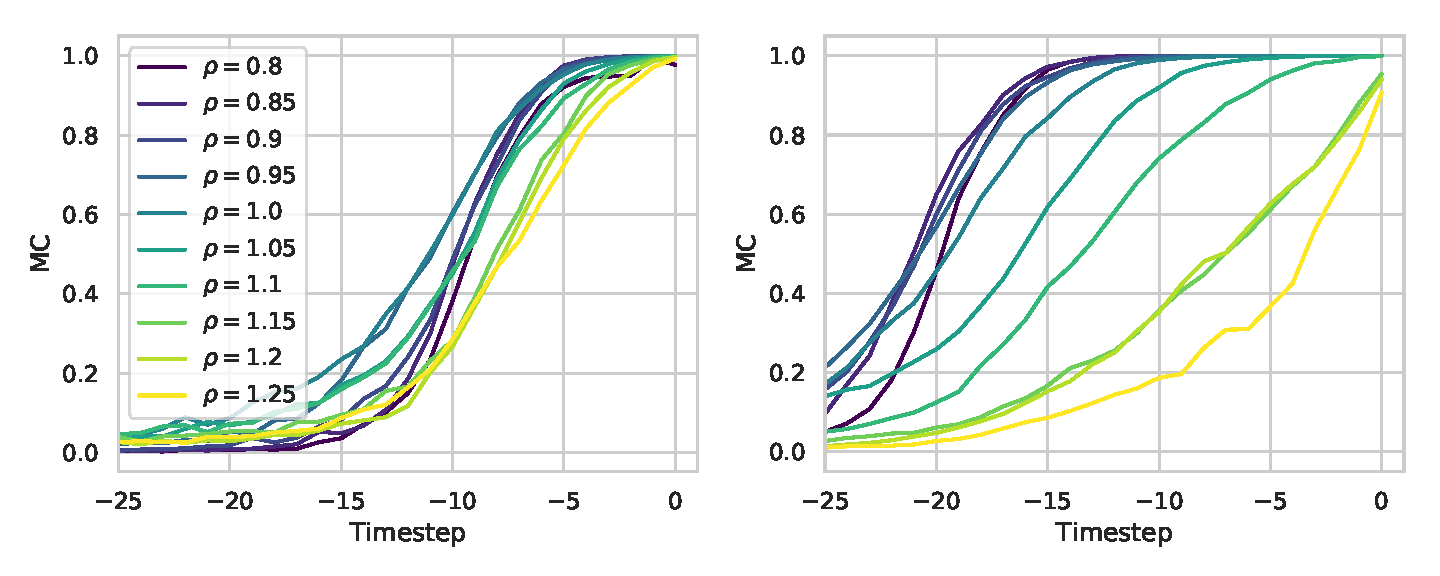
\includegraphics[width=\linewidth]{mc_seq.pdf}
  \caption{Determination coefficient over time for various spectral radii of
  the reservoir and two different learning algorithms. On the left the network
  was trained with GD and on the right with pseudo-inverse regression. The SGD
  trained network does not show a clear depedence on spectral radius, while in
  the LMS network it is clearly visible.}
  \label{fig:mc_seq}
\end{figure}

\begin{listing}
  \inputminted{json}{pseudocode/model_setups/memorize_setup.json}
  \label{lst:memorize_setup}
  \caption{ESN setup parameters for the memorization task. The \ttt{"False"}
    value of the Tikohnov regularization parameter $\beta$ means that the
    pseudo-inverse method was used. The spectral radius is varied from experiment
    to experiment.
  }
\end{listing}

To find the MC of the ESN it was trained with batches of $m=2000$ random
sequences.  Once with the Adam algorithm and once with the pseudo-inverse
method (which of course only need a single batch of random sequences to be
trained). After the training phase, another batch is fed to the network for
evaluation. An exemplary reconstruction is shown in
figure~\ref{fig:random_timeseries_recovery}.  It becomes evident that the most
recent time steps can be reconstructed almost perfectly and the memory of the
network becomes weaker further back in time.  With this setup one can try to
find the optimal spectral radius, which maximizes the memory capacity.  Both
plots in Fig.~\ref{fig:mc_seq} show the coefficient of determination over the
last 25 time steps at varying spectral radius $\rho$.  Interestingly, training
the ESN via a least mean squares approach (LMS, pseudo-inverse in this case)
seems to be much more efficient than training with Adam in this case.  In
addition, scaling $\rho$ has only a very small effect in the Adam-optimized
network, while it is clearly visible in the LMS ESN, but this is probably due
to the worse performance the SGD algorithm.  Figure~\ref{fig:mc_rho} suggests
that MC increases as $\rho$ approaches one and then quickly degenerates. This
is thoroughly investigated computationally in a paper by [\cite{farkavs2016}],
which in essence confirms the conjectures that were made before.

\begin{figure}
  \begin{minipage}[t]{.48\textwidth}
    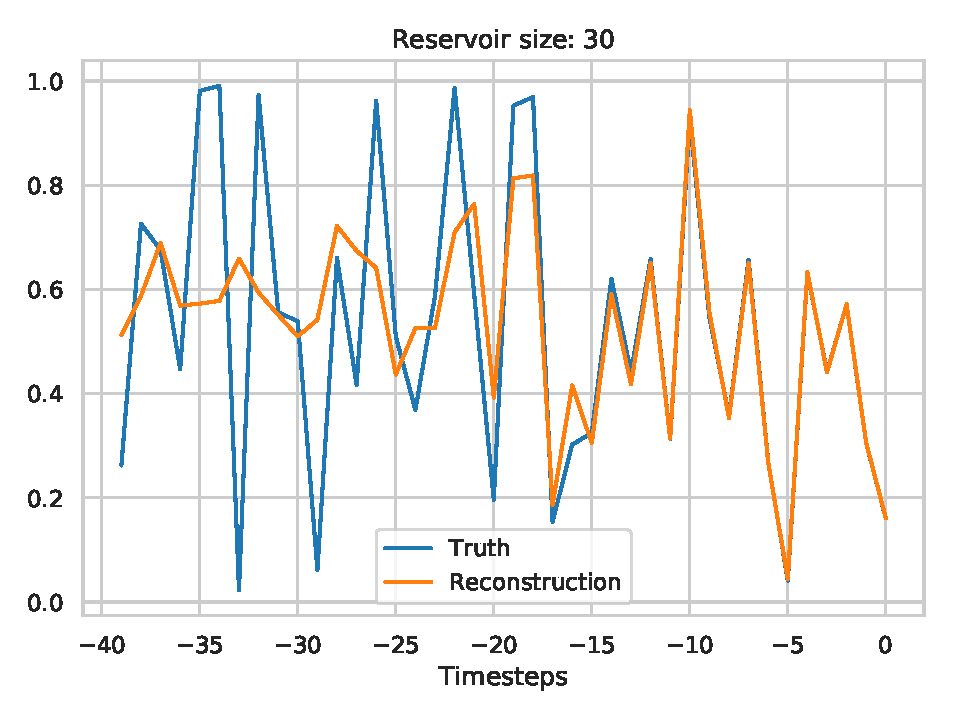
\includegraphics[width=\linewidth]{random_timeseries_recovery.pdf}
    \caption{
      True vs. reconstructed random time series. Most recent time step at $t=0$.
    }
    \label{fig:random_timeseries_recovery}
  \end{minipage}
  \hspace{.02\textwidth}
  \begin{minipage}[t]{.48\textwidth}
    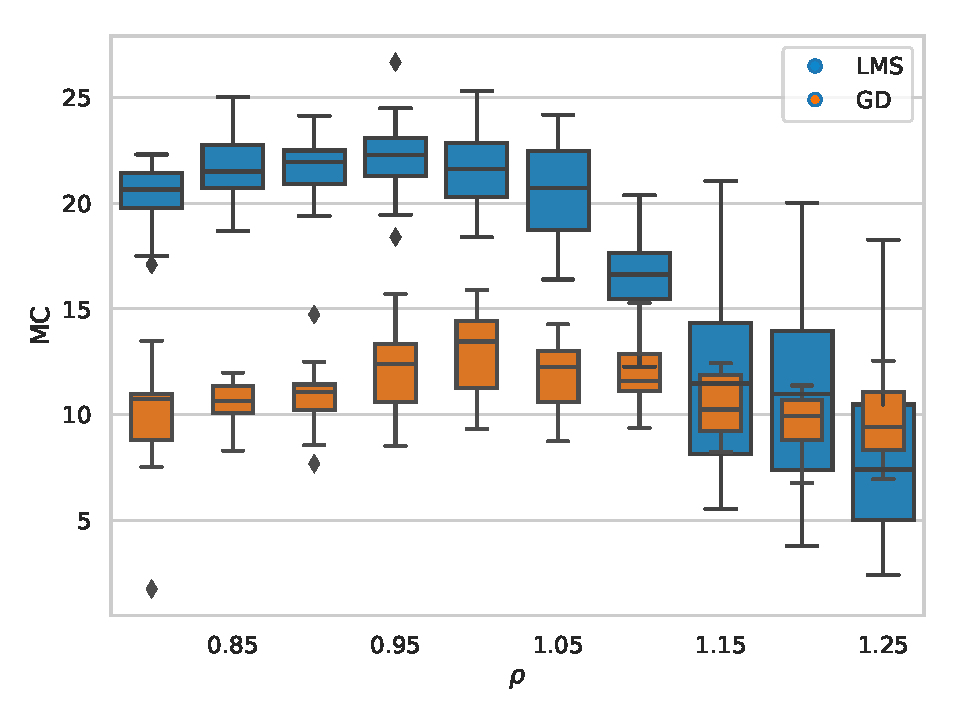
\includegraphics[width=\linewidth]{mc_rho.pdf}
    \caption{MC over spectral radius $\rho$ for the LMS and GD trained networks.}
    \label{fig:mc_rho}
  \end{minipage}
\end{figure}



\newpage
\section{Mackey-Glass System}%
\label{sec:res_mackey_glass_system}

\begin{figure}
  \centering
  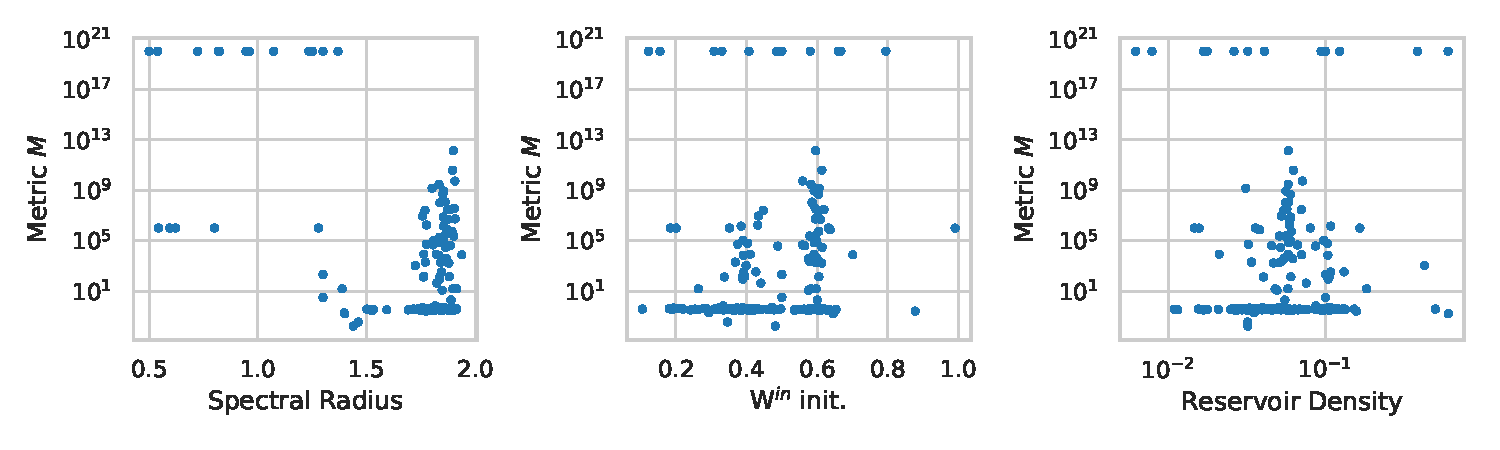
\includegraphics[width=\linewidth]{mackey_esn_ba_var_loss.pdf}
  \caption{Hyper-parameters over the squared error metric. The very large
    values are caused by diverging predictions that were clipped to a maximal
    $\mathrm{RMSE}=10^{20}$. The weight initialization and the sparsity
    parameters yield good performance in a certain range, the spectral radius
  only allows good performance for values larger than one.}
  \label{fig:mackey_esn_ba_var_loss}
\end{figure}


The first actual prediction task that will be solved by the ESN is the one of
the Mackey-Glass system that was described in
section~\ref{sec:mackey_glass_system}.  The reservoir is initialized with 500
units, which should be more than enough given that the period of the
considered time series is below 100 time steps, and that the ESN should have a
memory capacity slightly smaller than 500 steps.  The ESN is fed with a
sequence of length 2200, which creates the same number of internal states. To
avoid transients in the internal state, the first 200 steps are discarded. The
remaining 2000 internal states can be used to train the readout layer
$\wmatr{out}$ via the pseudo-inverse method. Three hyper-parameters (HP) remain
to be set: spectral radius, reservoir density, and input weight initialization
parameter, which are found with the help of Bayesian Optimization (BO).  For
this purpose, the package \ttt{scikit-optimize} was used to minimize the
RMSE
\begin{equation}
  \text{RMSE} = \frac{1}{N} \sum_{i=0}^N || d_i - y_i ||_2
\end{equation}
over several predictions.  The scikit algorithm needs an interval for every
parameter to form an HP space that it can sample from, which where chosen as
specified in table~\ref{tab:mackey_bo}. The resulting optimal HPs were obtained
over five BO runs.  Each BO run evaluated 100 trained ESNs at different points
in the HP space (Fig.~\ref{fig:mackey_esn_ba_var_loss}).  A surprising result
is that the optimal spectral radius is significantly larger than one.
In fact, the predicted signal just converges towards a value close to the mean
of the series if the spectral radius is close to one.
\begin{table}[h]
  \centering
  \rowcolors{2}{gray!25}{white}
  \begin{tabular}{|l c c c c|}
    \hline \rowcolor{gray!50}
    Parameter        & Best              & Min  & Max & Prior \\ \hline
    Spectral radius  & $1.40$   & 0.5  & 2.0 & uniform \\
    Weight init.     & $0.48$   & 0.1  & 1.0 & uniform \\
    Density          & $0.03$   & 0.01 & 1.0 & logarithmic \\
    \hline
  \end{tabular}
  \caption{Hyper-parameter results obtained via Bayesian Optimization}
  \label{tab:mackey_bo}
\end{table}

This is peculiar, as section~\ref{sec:short_term_memory} showed a spectral
radius close to one to be optimal for the memorization of sequences.  It
suggests that the crucial ingredient to predicting chaotic time series might
not only be a very good knowledge of the past, but something else. In fact this
is were the memory non-linearity tradeoff that was mentioned in
section~\ref{sub:short_term_memory} comes into play.  The more non-linear a
prediction task becomes the higher must the spectral radius of the reservoir be
to perform well. Unfortunately a large spectral radius degrades the MC of the
ESN. A mathematically sound framework for reasoning about the memory
non-linearity tradeoff is yet to be developed, but a rigorous computational
analysis of the problem is carried out in an article by [\cite{verstraeten2010}].
For the purpose of an anomaly detection it is enough that we found good
parameters for the prediction task. The quality of the predictions is depicted
in Fig.~\ref{fig:mackey1d_predictions}.
The predictive power of the ESN varies slightly over different parts of the
Mackey-Glass system. By randomly choosing different starting points in the
sequence and creating predictions for the next 500 frames, we can evaluate the
average error that the ESN makes at each frame.
Fig.~\ref{fig:mackey1d_predictions} shows the best and worst predictions in the
two upper plots and the average deviation of prediction and target in the
bottom.  An anomaly detection might be feasible within the first 100 frames, an
anomaly that is caught beyond that point might as well be caused by a degraded
prediction.\\

\begin{figure}
  \centering
  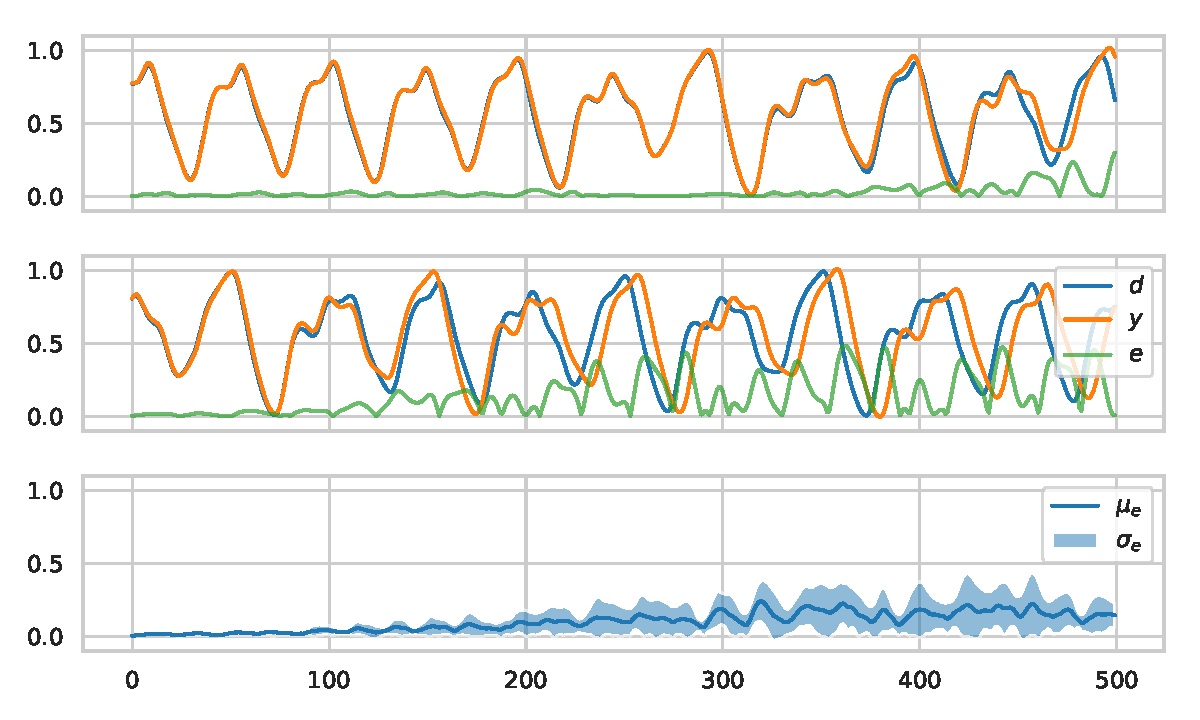
\includegraphics[width=\linewidth]{mackey1d_predictions.pdf}
  \caption{The best (top) and worst (middle) predictions from 20 randomly
    chosen starting points of the Mackey-Glass series. All predictions were
    made by an ESN with optimal hyper-parameters.  The target values $d$ are
    shown in blue, prediction $y$ in yellow, and the error $e = |d - y|$ in
    green. The plot in the bottom shows the variability of $e$ over different
    predictions.
  }
  \label{fig:mackey1d_predictions}
\end{figure}


At this point, \emph{finally}, all necessary parts to try and find artificially
introduced anomalies in the MG system are in place. The anomalies are created
by varying the parameter $\gamma$ of the MG Eq.~\ref{eq:mackey_glass}.  By
default it has a value of $\gamma = 0.1$.  Every 400 steps it is decreased by
an amount $\delta$ set back to its initial value after 50 steps. Depending on
the magnitude of $\delta$ this creates rather smooth looking anomalies. Easily
visual anomalies are created with a value of $\delta = 0.05$. To search the
outliers, the trained network receives a sliding window of 300 steps of the
anomalous sequence.  The predictions for the next $N_p = 50$ steps into the
future are collected and the \emph{mean prediction error} (MPE) is calculated
for every sequence that was fed to the ESN:
\begin{equation}
  \text{MPE} = \frac{1}{N_p} \sum_{t=1}^{N_p} | d_t - y_t |.
\end{equation}
The MPE is recorded for the whole dataset and the normality score $\Sigma$
(Eq.~\ref{eq:normality_score}) is computed with a large window size of 100
steps and a small window size of 5 steps..  The result is shown in
Fig.~\ref{fig:mackey_visible_anomalies}. With delight we can find that all
anomalies are easily caught.  To demonstrate the capabilities of the ESN to
efficiently find outliers in chaotic systems like the MG system,
Fig.~\ref{fig:mackey_anomalies} depicts how the algorithm performs on
anomalies that would, most probably, not be spotted by a human.

\begin{figure}
  \centering
  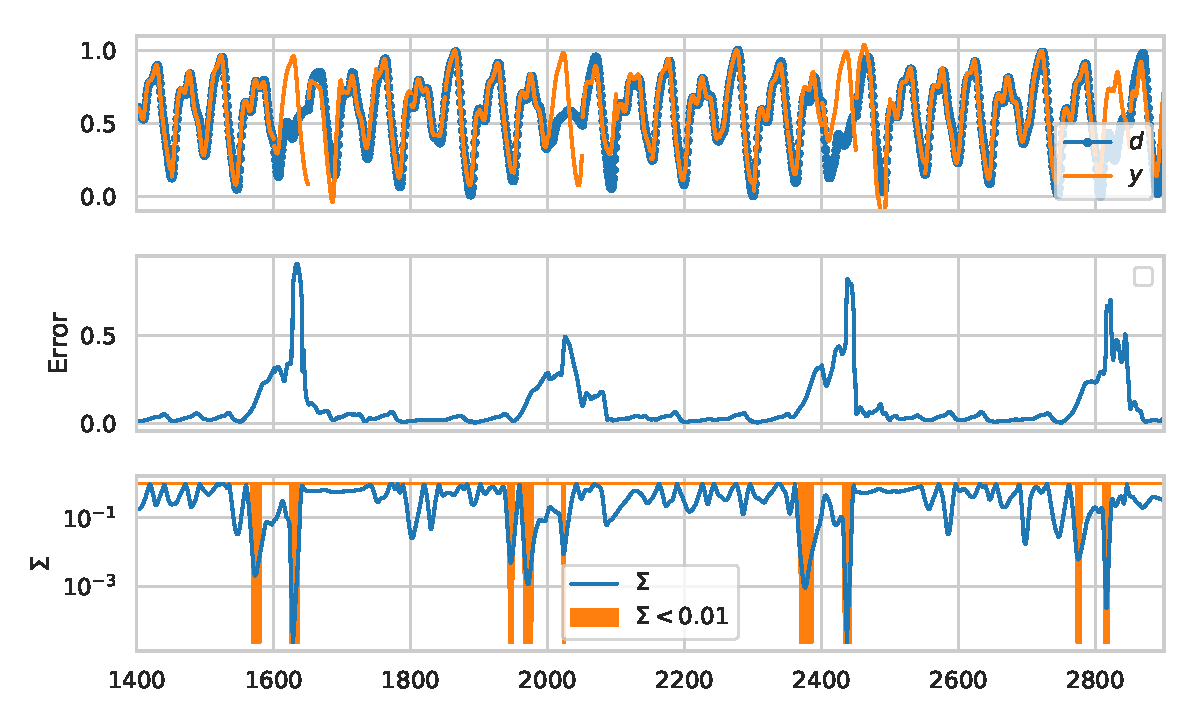
\includegraphics[width=\linewidth]{mackey_visible_anomalies.pdf}
  \caption{Mackey Glass system with artificially introduced anomalies at every
    400th step with $\delta=0.05$. The detected anomalies are indicated by the
    yellow bars in the plots of the score $\Sigma$. The anomaly score catches
    the irregularly high error regions slightly too early, because the
    prediction error goes up as soon as the prediction window reaches into the
  anomalous regions.}
  \label{fig:mackey_visible_anomalies}
\end{figure}

\begin{figure}
  \centering
  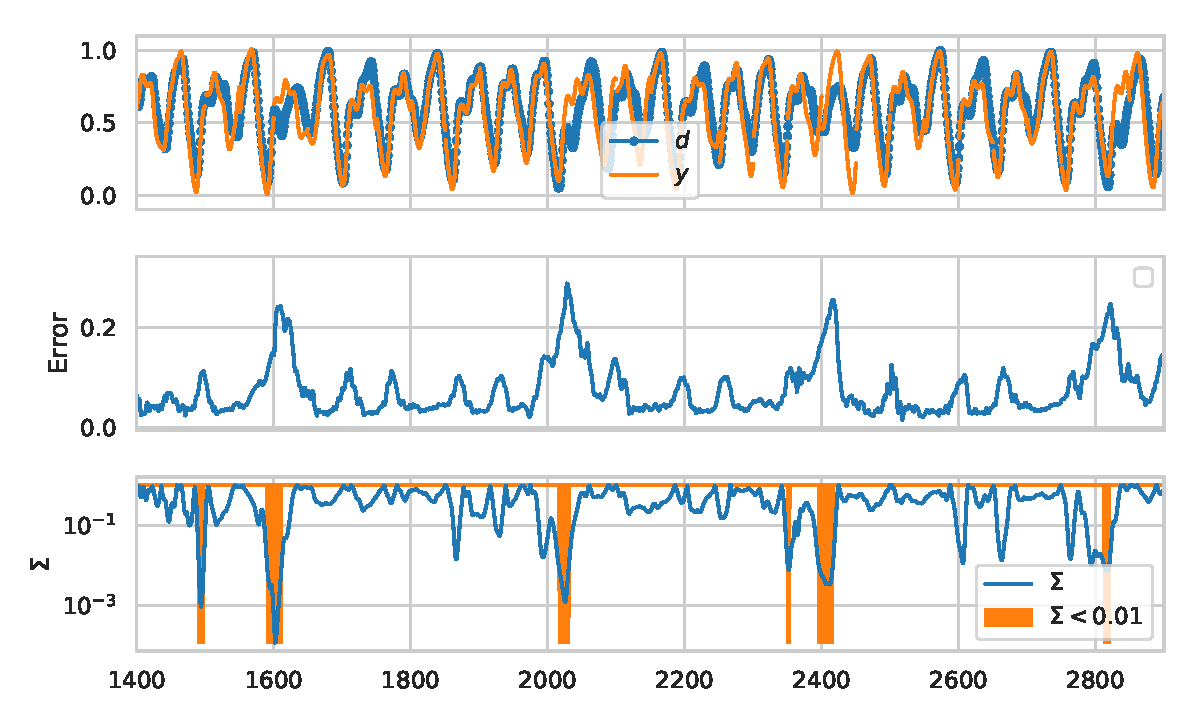
\includegraphics[width=\linewidth]{mackey_anomalies.pdf}
  \caption{Outliers that would have probably not been caught by humans. Created
  with $\delta = 0.03$. One false positive at $t=1500$.}
  \label{fig:mackey_anomalies}
\end{figure}

\begin{listing}
  \inputminted{json}{pseudocode/model_setups/mackey_setup.json}
  \label{lst:mackey_setup}
  \caption{ESN setup parameters for MG prediction.}
\end{listing}






\clearpage
\section{Dansgaard-Oeschger Events}%
\label{sec:res_dansgaard_oeschger_events}

The second dataset consisting of ice-core records that reach back 100k years
has two components. The $\delta^{18}$O sequence, which is directly connected to
surface temperature and the Ca$^{2+}$ series, that measures dust content and
shows similar patterns.  Both sequences lack a clear reappearing pattern, which
was clearly visible in the Mackey-Glass series, despite the chaotic nature of
the MG system. This makes a one time training over a part of the dataset that
contains most of variability impossible.  It should however still be possible
to project several dozen years ahead by moving to an online learning mode. In
the online mode, the output weights are recomputed with every new time slice
that is fed to the network.  The resulting short-term predictions $y$ are shown
in Fig.~\ref{fig:d18O_anomalies}.
\begin{listing}
  \inputminted{json}{pseudocode/model_setups/DO_setup.json}
  \label{lst:DO_setup}
  \caption{ESN setup parameters for DO event detection. The hyper-parameters were
  found via Bayesian Optimization.}
\end{listing}
They were achieved by training the ESN for 1500 input steps and predicting the
next 200 steps (the time step of the series is one year). Due to the very
irregular dataset the predictions are not very good, but at points where the
sequences change abruptly they deviate much more from the target values than
they do otherwise. This can be exploited to detect the DO events which are
located exactly at these abruptly changing points. Apart from the online weight
adaption, the procedure is the same as with the MG system. The score is
calculated from the MPE and thresholded, resulting in the detection of
anomalies at the yellow colored regions of Fig.~\ref{fig:d18O_anomalies}.
Abrupt changes after steady periods are easily detected by the algorithm.  DO
events that lie close to each other tend to slip through. This is due to the
fact that the ESN learns from the previous DO events and as it is trained on
these anomalies, they are considered normal.
\begin{figure}
  \centering
  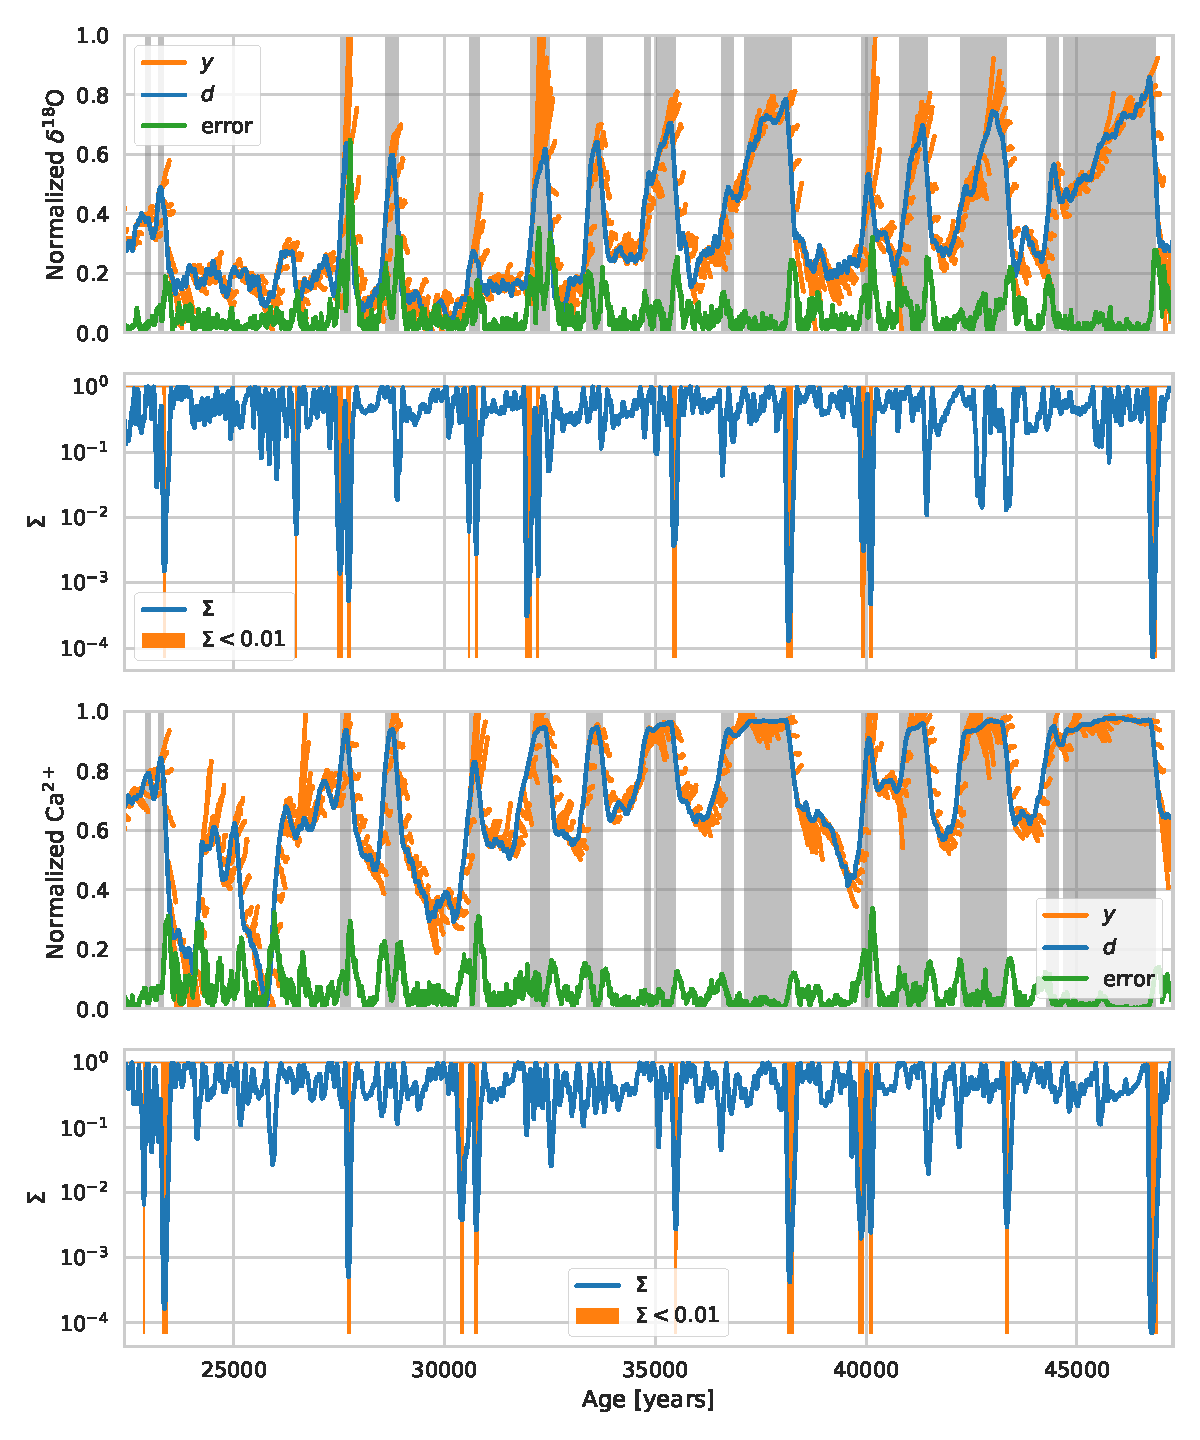
\includegraphics[width=\linewidth]{d18O_Ca2_anomalies.pdf}
  \caption{Results of the DO dataset. The DO events are marked with
  the grey background. Detected anomalies are indicated by the yellow bars in
  the plots of the normality score $\Sigma$}
  \label{fig:d18O_anomalies}
\end{figure}




\newpage
\section{Kuroshio}%
\label{sec:res_kuroshio}
\begin{figure}
  \begin{minipage}[b]{0.5\linewidth}
    \centering
    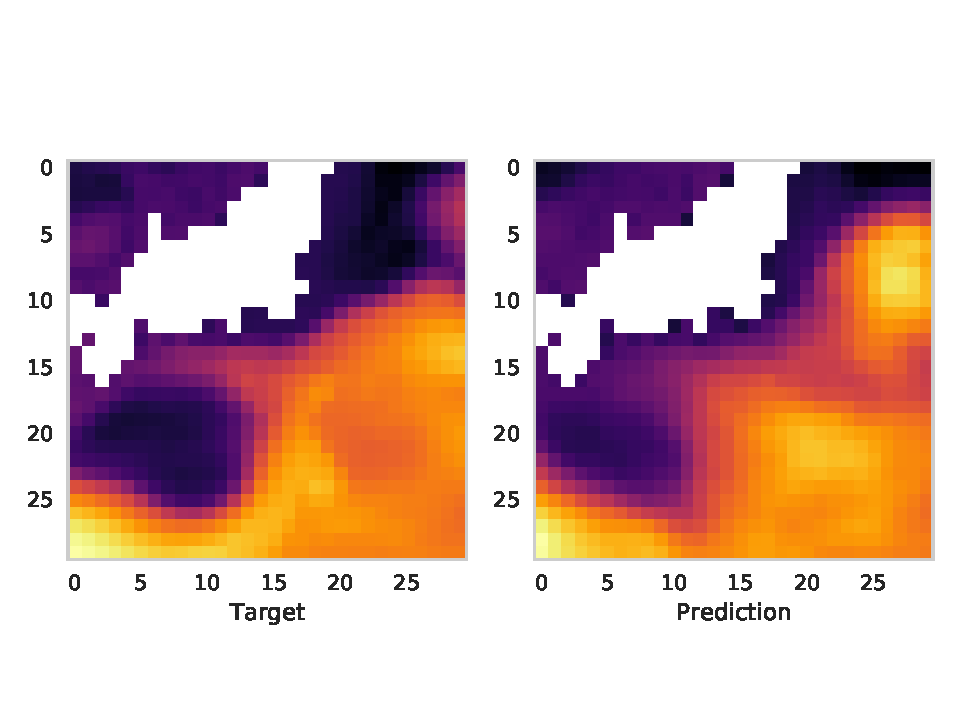
\includegraphics[width=.9\linewidth]{kuro_example_pred_stepidx200.pdf}
  \end{minipage}%% 
  \begin{minipage}[b]{0.5\linewidth}
    \centering
    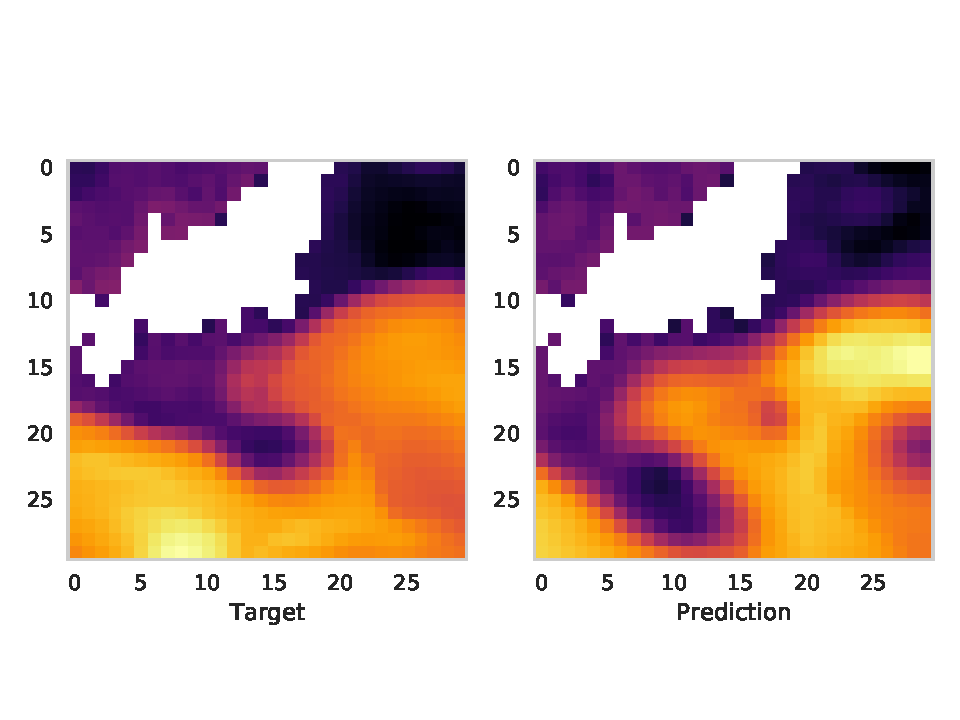
\includegraphics[width=.9\linewidth]{kuro_example_pred_stepidx470.pdf}
  \end{minipage} 
  \begin{minipage}[b]{0.5\linewidth}
    \centering
    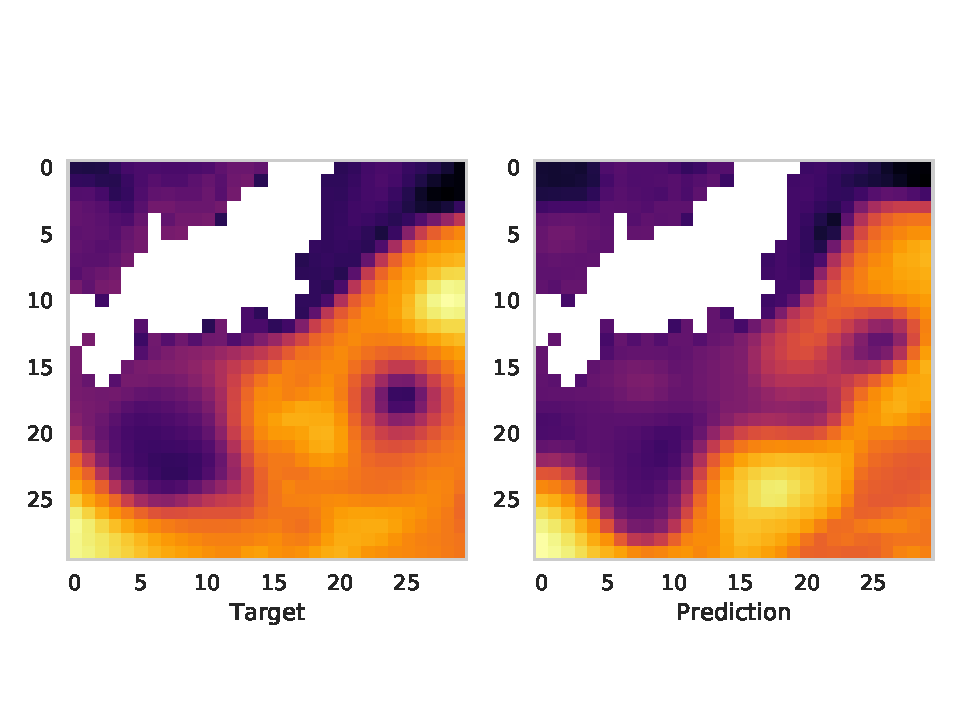
\includegraphics[width=.9\linewidth]{kuro_example_pred_stepidx0.pdf} 
  \end{minipage}%%
  \begin{minipage}[b]{0.5\linewidth}
    \centering
    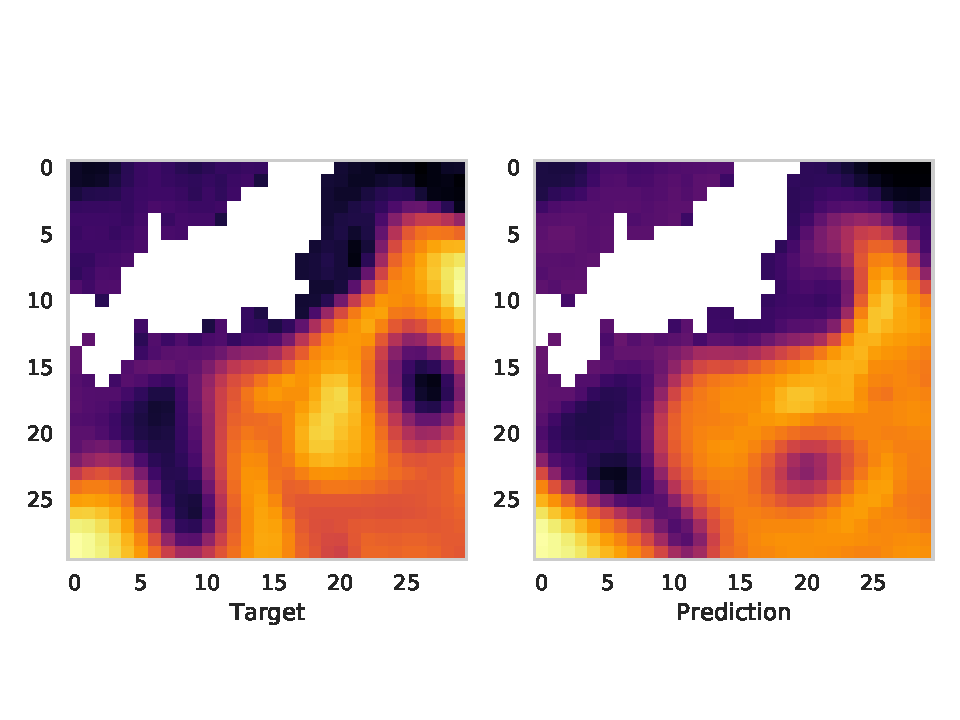
\includegraphics[width=.9\linewidth]{kuro_example_pred_stepidx100.pdf}
  \end{minipage} 
  \caption{Four exemplary predictions and corresponding desired outputs in the
    Kuroshio region. Shown is the 150th predicition frame out of 200.}
  \label{fig:kuro_pred_examples} 
\end{figure}


The prediction of the Kuroshio region involves significantly more data that
needs to be processed by the ESN. This means that the reservoir size has to
grow appropriately.  As a rule of thumb, the size of the internal state
$\vt{x}$ should be at least as big as the period of the dataset is long. The
most obvious period in climate simulations is typically the annual signal
which, in our case of 3-day means, is 122 steps long. To be able to remember
whole video sequences, this number should be multiplied by the number of pixels
in each frame to obtain the state size. Even if we consider raw inputs of 100 x 100
pixels and resample them to a size of 30 x 30, this would still result in a
state size greater than 100 000, which would result in a memory use of more
than 40 GB of the internal square reservoir matrix alone. This is clearly
unacceptable. Luckily, the pixels are highly correlated and we can hope that
the ESN is able to compress some of the information of the input images it
receives. Sizing the reservoir down to 10000 units and keeping it very sparse
will decrease the memory usage of the network to an acceptable amount of a few
hundred MB.

\begin{figure}[p]
  \centering
  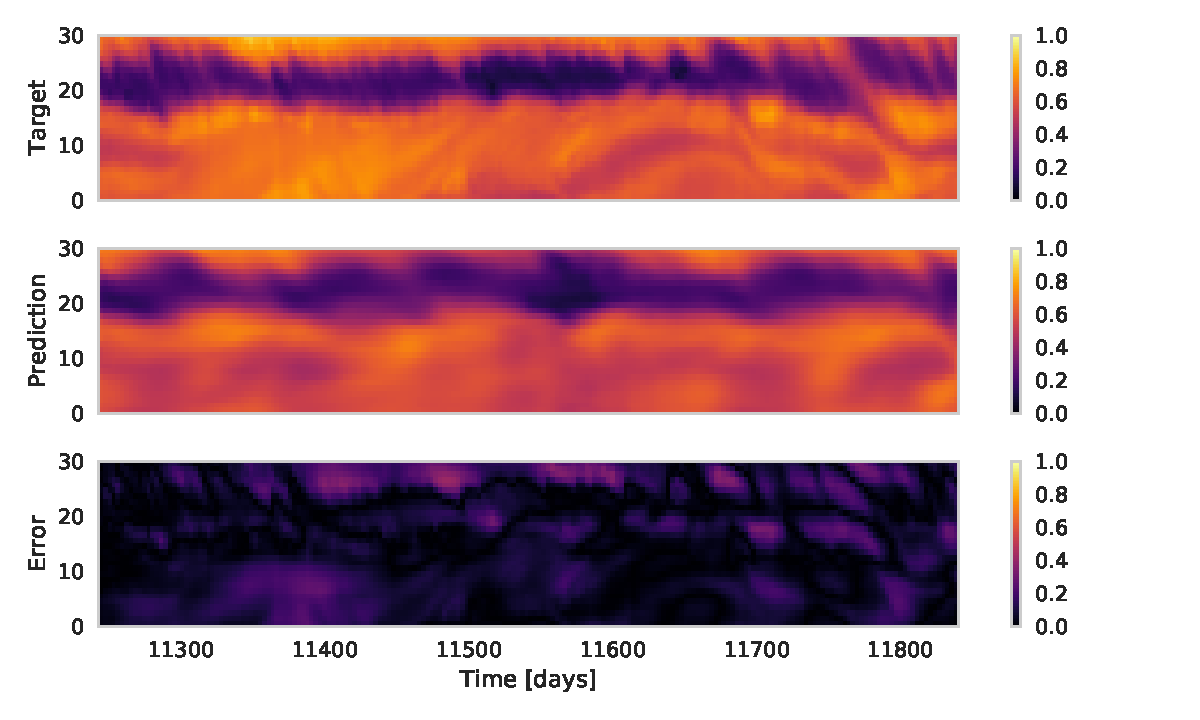
\includegraphics[width=1.1\linewidth]{kuro_pred_stepidx290}
  \caption{Exemplary prediction 200 steps into the future.}
  \label{fig:kuro_pred_stepidx290}
\end{figure}

\begin{figure}[p]
  \centering
  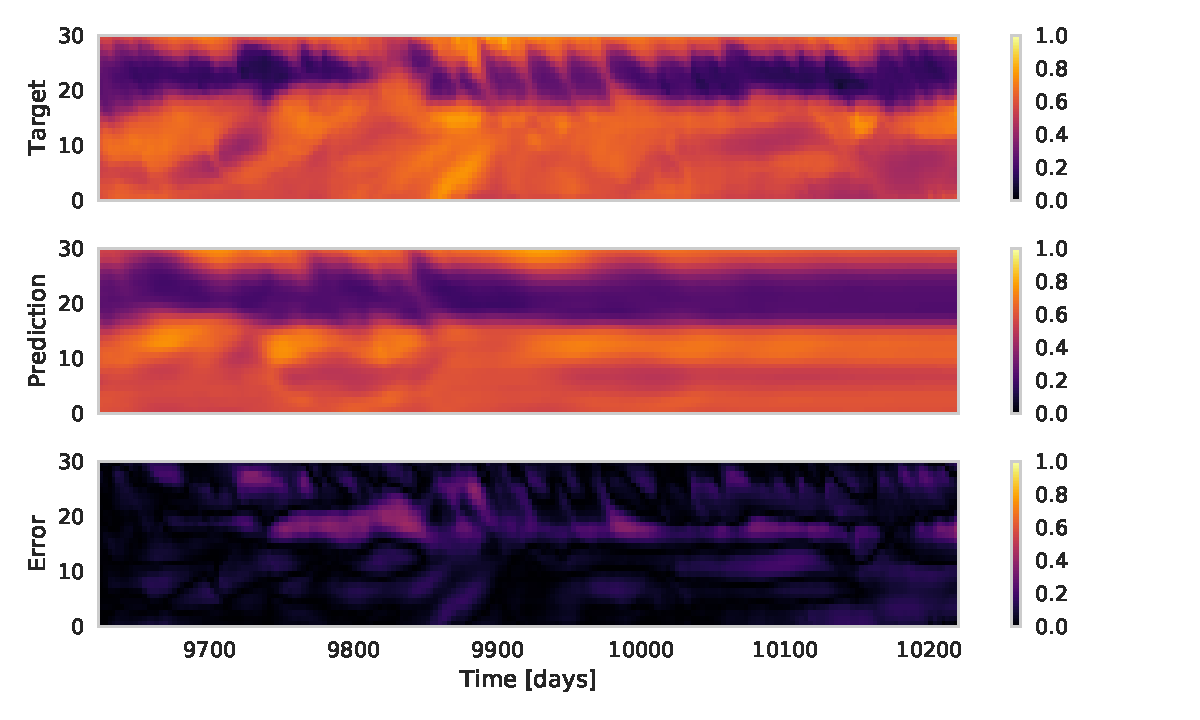
\includegraphics[width=1.1\linewidth]{kuro_pred_stepidx20}
  \caption{Another prediction example. Here it looks like the internal state of
  the ESN has reached a fixed point, so the prediction remains constant after
  day 10100.  This fixed point interestingly produces predictions that are very
  similar to the mean contracted state of the Kuroshio, if viewed in 2D.}
  \label{fig:kuro_pred_stepidx20}
\end{figure}



Apart from using a sparsely represented ESN reservoir, the approach is again
the same as before.  The ESN receives 1300 input frames and predicts the next
200, which amounts to a prediction of roughly two years. Exemplary predictions
and the corresponding desired target outputs are shown in
Fig.~\ref{fig:kuro_pred_examples}. The figures ~\ref{fig:kuro_pred_stepidx290}
and ~\ref{fig:kuro_pred_stepidx20} show the 25th row of two more exemplary
target and prediction evolutions over time. The prediction error that is shown
is quite low for the predicted two years, but just to be sure only the first
year, meaning the first $N_p = 100$ frames, will be used for the subsequent
anomaly detection.

Fig.~\ref{fig:kuro_mean_pred} compares the target and prediction values for the
last prediction step ($N_p=100$) that is considered for the anomaly detection.
The error plot shows the MPE for each prediction. A large deviation of
prediction and target is visible around day 15500. The normality score (plotted
in a logarithmic color scale) that was calculated from the MPE sequence is very
low in this region as well. It seems to be a promising candidate for the
Kuroshio anomaly. By summing up all instances where the anomaly score $\Sigma <
0.01$ we can create a map of outliers. The result is shown in
Fig.~\ref{fig:kuro_anomaly_count}.  It shows a region with a lot of outliers
just where we expect them to be.  The similarity between the anomaly count and
the difference of elongated and contracted states is obvious and the result
will be regarded as a successful detection of the Kuroshio anomaly.

The second region of high anomaly counts is where the Kuroshio turns towards
the North Pacific basin. This anomaly is caused by a large unpredicted  eddy
that enters the analyzed area from the East. This anomalous region would
probably vanish if the analysis area is shifted eastward, away from Japan.
This would be the obvious next step of the outlier search, but unfortunately a
thorough analysis of the whole world is out of the scope of this work and will
remain as one path that a further studies of this problem could take.
\begin{figure}
  \centering
  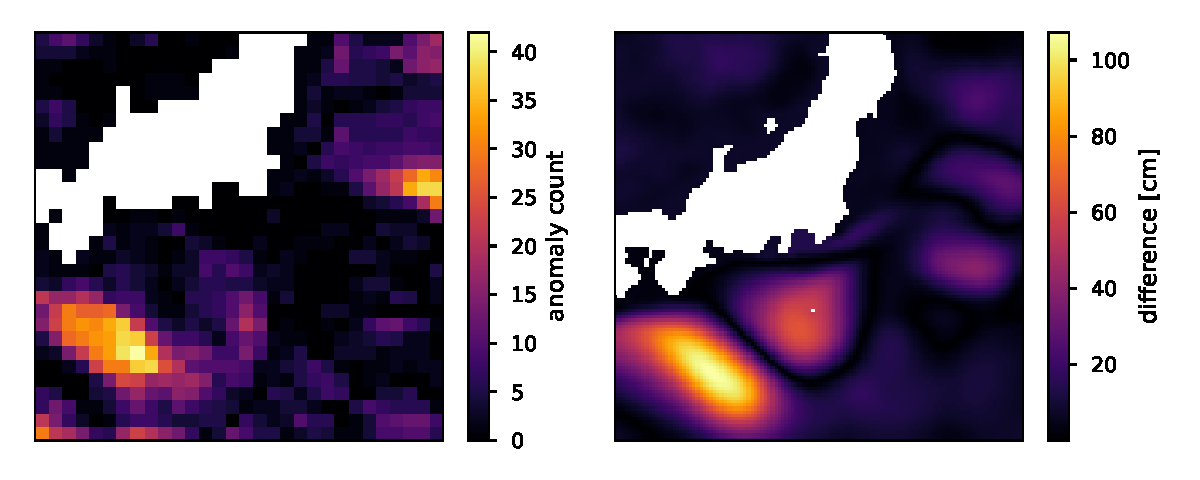
\includegraphics[width=\linewidth]{kuro_anomaly_count.pdf}
  \caption{Count of all pixels with a normality score that is lower than 0.01,
  compared to the assumed true form of the Kuroshio anomaly (obtained from the
  difference of its two states).}
  \label{fig:kuro_anomaly_count}
\end{figure}


\begin{figure}
  \centering
  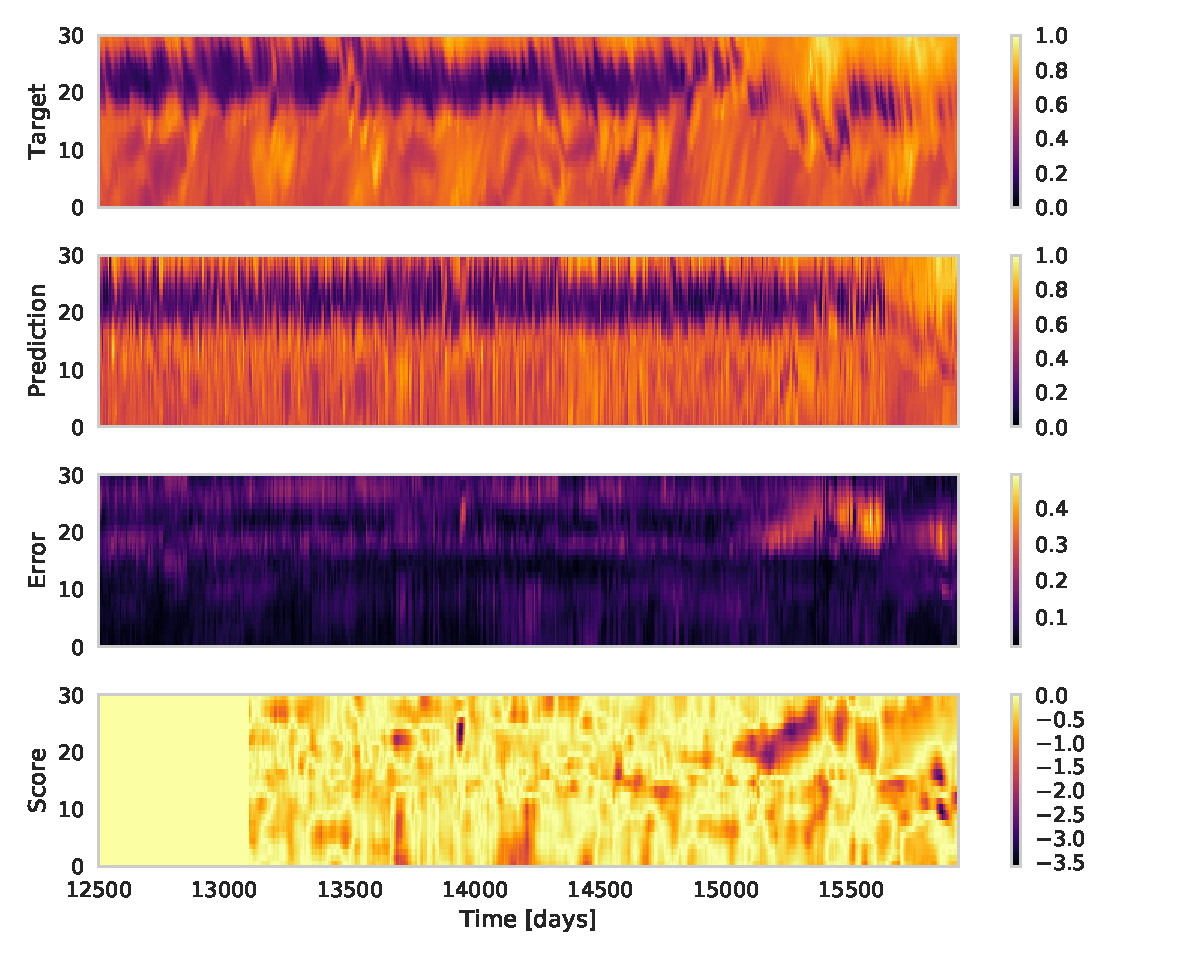
\includegraphics[width=1.1\linewidth]{kuro_mean_pred.pdf}
  \caption{The target plot shows the true values of one row of the SSH
    frames that were fed to the ESN.  In the prediction plot we can see the
    prediction that was made based on the internal state 100 steps before.
    The error plot depicts the mean error of one prediction sequence and in the
    bottom we can see the resulting anomaly score on a logarithmic color scale.
  }
  \label{fig:kuro_mean_pred}
\end{figure}

\begin{listing}
  \inputminted{json}{pseudocode/model_setups/kuro_setup.json}
  \label{lst:kuro_setup}
  \caption{ESN setup parameters for Kuroshio anomaly detection. The Bayesian
  Optimization resulted a large range of parameters with similar performance as
  long as the spectral radius was larger than 1.3 and the weight initialization
  parameter larger than 0.8. The chosen hyper-parameters reflect the need for a
  sufficiently non-linear reservoir.}
\end{listing}

\chapter{Conclusions \& Further Work}
\label{cha:future_work}
\epigraph{This chapter wraps up this thesis and gives some suggestions
  towards eventual future work. It briefly discusses how the developed
  model could be scaled to almost arbitrarily large datasets and how the
  forecasting network could be improved with respect to prediction and
  computational performance.
}

\section{Conclusions}%
\label{sec:conclusions}

After a considerable amount of thought was put into the understanding of the
dynamical nature of ESNs and recurrent neural networks in general, I
successfully implemented a framework that is able to predict high-dimensional,
spatio-temporal, chaotic time series.  It can be concluded from
chapter~\ref{cha:results}, that an automated detection of
anomalies in chaotic systems is possible. The application of the
ESN to the prediction problem has lead to a very cost efficient search
algorithm, which is quite striking, considering that it is able to create said
chaotic predictions.

The generality of the prediction framework is another notable point.  The
problem of predicting a chaotic system long enough to detect anomalies was
solved without making any assumptions about the underlying physics.  The only
adjustments that have to be made from one dataset to the next are a few
hyper-parameters. Both the state size and the spectral radius of the ESN can be
chosen within narrow bounds by examining the requirements of the problem. The
state size should be at least as large as the period of the examined sequence
and the spectral radius must be large enough to capture its non-linearity.
However, to achieve the best results the exact choices of hyper-parameters are
best left to algorithms such as Bayesian Optimization.  This reduces the amount
of tweaking that has to be done to apply the model to new datasets to a
minimum.

The second goal of finding new physical behaviour in the available climate
model output remains to be achieved. It will require some house keeping in the
analysis part of the code, but all the necessary parts are in place.

With this proof of concept we have shown that the concepts of machine learning
can be of much use in the field of oceanography and climate physics as a whole.
A wider application of the concepts from artificial intelligence and machine
learning promises to make the full potential of climate data exploitable in
completely new ways.



\section{Future Work}%
\label{sec:future_work}

The ultimate goal of this work was to create an algorithm that skims through
huge ocean simulation datasets and returns interesting areas to search for new
physical behaviour. To achieve this, the created anomaly detection, which
can currently process small windows, has to be scaled to work on the large,
global domain. This can be achieved by running many ESNs in parallel over -
possibly overlapping - small windows of the global domain.

Of course, also the current  prediction model can be improved. There is still
much room for improvement by increasing the complexity of the ESN. This would,
most probably, reduce the amount of false positives of the detection.
Additionally, the performance of the ESN could benefit tremendously from
implementing it with a different framework than Tensorflow.

\subsection{Scaling To The Global Domain}%
\label{sub:scaling_to_the_global_domain}

By applying the detection algorithm to small windows of the model output, many
independent ESNs can be run in parallel. This can be scaled until the memory
limitations of the available computing resources are reached.
This spatial parallelization would enable the analysis of the full, global domain.

The parallel ESNs can either operate independently within their window, or the
predictions can be processed into one large super-prediction. For this the
windows must, of course, overlap, which introduces a considerable amount of
communication between the parallel ESN instances into the problem. The
super-prediction can subsequently be divided back into the windows that are fed
back to the individual ESNs. Should physical memory (not STM) become a problem in
the super-prediction approach, the number of individual reservoirs could be
reduced by sharing the large reservoir matrix and only having individual output
weights for each sub-prediction.

The super-prediction approach would also reduce boundary effects like the
large unexpected eddy that entered the Kuroshio prediction window.


\subsection{Predictor Improvements}

With the rather basic setup of a single ESN cell as the prediction network,
there is still much room for improvements of the prediction model itself.  The
most obvious of which would be to add convolutional layers in front of the ESN
cell. This could lead to significant improvements by leveraging the spatial
information of the input as described in
Sec.~\ref{sub:convolutional_neural_nets}. This would mean that convolution
filters have to be learned and make an expensive GD algorithm for the weight
optimization necessary. However, it might be possible to leverage random
convolutional layers in a similar fashion like the reservoir of the ESN does.
Networks that contain untrained feedforward layers are called \emph{extreme
learning machines} and were introduced by [\cite{huang2006}].  The combination
of the two concepts was introduced by [\cite{butcher2013}] and termed
\emph{reservoir with random static projections} (R$^2$SP).  This architecture
promises to solve the memory non-linearity tradeoff by separating non-linear
transformation and internal memory of the network and could thus be much more
powerful.

\begin{figure}
  \centering
  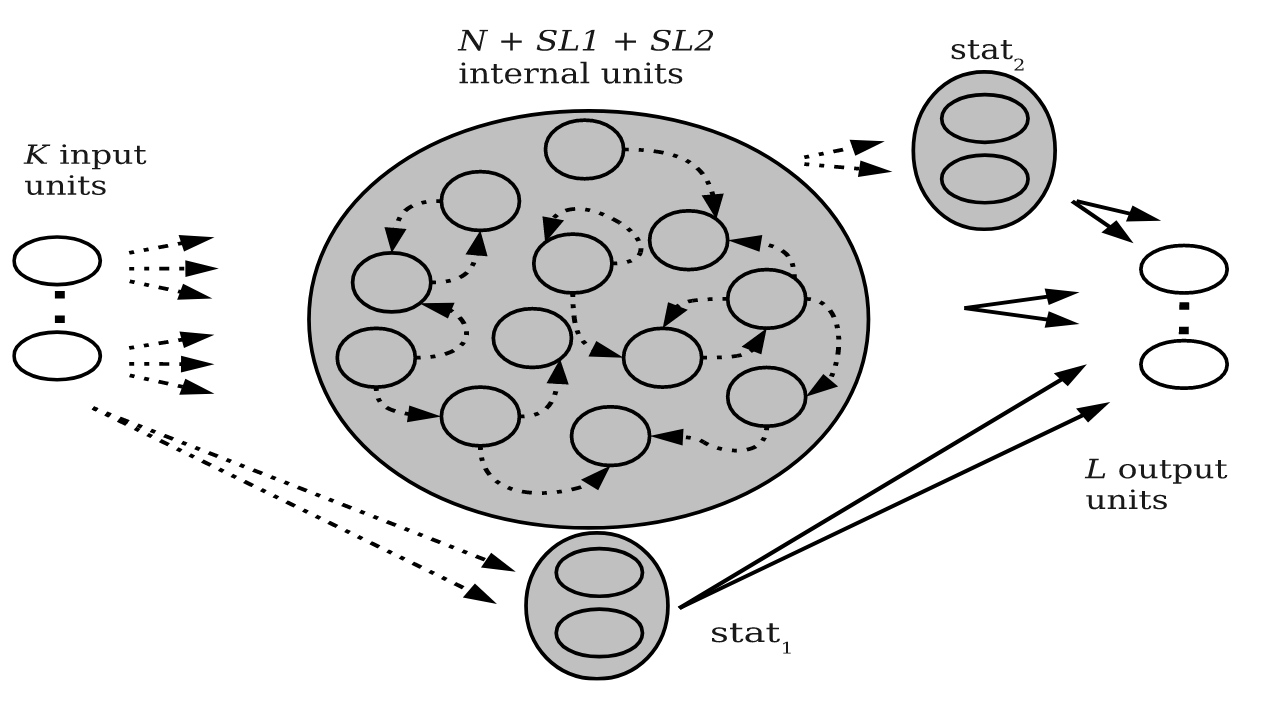
\includegraphics[width=0.6\linewidth]{r2sp.png}
  \caption{Reservoir with random static projections [\cite{butcher2013}]. The
  stat$_1$ and stat$_2$ layers are static feedforward layers, that take the
  part of the non-linear transformation.  The recurrent internal units
  represent the memory of the network. Their reservoir matrix can be
  initialized with a spectral radius close to one to maximize memory without
  the need of introducing non-linearities.}
  \label{fig:r2sp}
\end{figure}

Another interesting approach to improve the performance of the network would be
to employ \emph{evolutionary optimization} techniques [\cite{fogel1997}] to find
a good reservoir matrix $\wmatr{}$ which could be reused for the whole ocean
dataset.  This would eliminate fluctuations in prediction performance from run
to run.


\subsection{Performance Improvements}
Probably the greatest advantage of the presented approach is its low computational
demand. Creating predictions of a few hundred frames for a window of 30x30
pixels does not take longer than a few seconds on a standard laptop.  However,
for a truly automated application of the model to very large datasets with long
sequences it would be interesting to implement it in another framework.
Tensorflow does not excel in RNN computations and it would be quite simple to
implement the network, for example, in Numpy and parallelize it with Bohrium
[\cite{bohrium}]. This would get rid of a lot of overhead that is caused by the
dynamic graph creation that Tensorflow is doing.

Additionally, the ESN, due to its static nature, holds the potential of being
compiled to an FPGA, which could improve performance even further.


\subsection{Understanding Recurrent Networks}
To date, the general understanding of the ESN and RNNs in general is not very
good.  It is assumed that an RNN classifier needs as many fixed points as it
has features to separate, but a fundamental understanding is still lacking.  A
further investigation of the influence of fixed-points and period cycles within
the internal state evolution on the memory and predictive capabilities of RNNs
would be very interesting.  This could lead to a more solid understanding of
how the hyper-parameters of the ESN are influencing its performance.


\appendix
\chapter{Derivations}
\label{app:derivations}
\newpage

\section{Spectral Radius}
\label{sec:spectral_radius}

The spectral radius is a key parameter that determines some properties of the 
echo state network weight matrix, which we will here denote as
$\matr{A} \in \mathbb{C} ^{n\times n}$.
If $\matr{A}$ has eigenvalues $\lambda_1, ... , \lambda_p$, where $p \leq n$,
the spectral radius is defined as
\begin{equation}
  \rho(\matr{A}) = \max \{|\lambda_1|,...,|\lambda_p|\}.
\end{equation}

Thus, to obtain the spectral radius we somehow have to find a reasonably close estimate
for the absolute largest eigenvalue.
For very large matrices, it obviously becomes infeasible to calculate all eigenvalues
which has a computational complexity of $O(n^3)$.
One method of quickly computing the largest eigenvalue is called \textbf{inverse iteraion}
(or inverse power method), but before diving into the exact algorithm we will go
through a quick recap of the linear algebra that is necessary for inverse iteration.

If the matrix $\matr{A}$ is diagonalizable, we can find a matrix $\matr{S}$ such that
\begin{equation}
  \label{eq:diagonal_matrix}
  \matr{A} = \matr{S}^{-1} {\Lambda} \matr{S},
\end{equation}
where $\Lambda$ is a diagonal matrix containing the eigenvalues
$\lambda_1,...,\lambda_p$.
From Eq.~\ref{eq:diagonal_matrix} follows that:
\begin{equation}
  \label{eq:matrix_power}
  \matr{A} \matr{A} = (\matr{S}^{-1}\Lambda\matr{S})(\matr{S}^{-1}\Lambda\matr{S})
                    = \matr{S}^{-1}\Lambda^2\matr{S},
\end{equation}
which means that for any continuous function one can write:
\begin{equation}
  f(\matr{A}) = \matr{S}^{-1} f(\Lambda) \matr{S},
\end{equation}
because every continuous function can be approximated by a polynomial function.
In our case it will turn out to be very useful, that
\begin{equation}
  \label{eq:inverse_ev}
  (\matr{A} - \sigma \mathbb{I})^{-1} =
        \matr{S}^{-1} (\Lambda - \sigma \mathbb{I})^{-1} \matr{S},
\end{equation}

because only the eigenvalues (on the diagonal of $\Lambda$) are affected by
the inversion, but the eigenvectors stay exactly the same.


\subsubsection{Power Method}
\label{ssub:power_method}
Suppose $\vec{x} \in \mathbb{C} ^n$, that can be written as the sum of eigenvectors
and eigenvalues:

\begin{equation}
  \vec{x} = \lambda_1\vec{e}_1 + ... + \lambda_p\vec{e}_p,
\end{equation}

where $|\lambda_1| > |\lambda_2| > ... > |\lambda_p|$ it follows that:
\begin{equation}
  \label{eq:sum_ev}
  \matr{A}^j \vec{x} = \lambda_1^j\vec{e}_1 + ... + \lambda_p^j\vec{e}_p,
  =  \lambda_1^j \sum_{i=0}^{p} \bigg(\frac{\lambda_i}{\lambda_1}\bigg)^j \vec{e}_i,
\end{equation}

which means that for large enough $j$ Eq.~\ref{eq:sum_ev} converges to:
\begin{equation}
  \label{eq:power_method}
  \vec{\mu} = \matr{A}^j \vec{x} \rightarrow \lambda_1^j \vec{e_1}.
\end{equation}

Eq.~\ref{eq:power_method} is called the \textbf{power method} for finding eigenvalues.
From the estimate $\vec{\mu}$ of the largest eigenvector one can easily obtain the estimate
$\sigma$ of the corresponding eigenvalue by applying the Rayleigh quotient:
\begin{equation}
  \label{eq:rayleigh_quotient}
  \sigma = \frac{\vec{\mu}^* \matr{A} \vec{\mu}}{||\vec{\mu}^* \vec{\mu}||}
\end{equation}

From Eq.~\ref{eq:sum_ev} one can quickly see that it has an error of $O(|\lambda_2/\lambda_1|^j)$,
which means that it converges very slowly if the two largest eigenvalues are very
close to each other.


\subsubsection{Inverse Iteration}
\label{ssub:inverse_iteration}
The inverse iteration method aims to solve the problem of slow convergence of the
power method by manipulating the eigenvalues of the iterated matrix favourably.

Suppose we can find a reasonably close estimate $\sigma$ of an eigenvector $\lambda_i$
of $\matr{A}$, then the matrix $(\matr{A} - \sigma \mathbb{I})$ is almost singular,
because on of the elements of its diagonalized counterpart is close to zero.
\footnote{The estimate $\sigma$ is often called shift, which is why this method is also known
as the \textit{inverse shift method}.}
This means, according to Eq.~\ref{eq:inverse_ev} that
$(\matr{A} - \sigma \mathbb{I})^{-1}$ has one very large eigenvalue,
which we can exploit for a fast conversion of the power method.
Starting from a random vector $\vec{x}_0$, the iterative update equation for the
inverse power method reads:
\begin{equation}
  \label{eq:inverse_iteration}
  \vec{x}_{i+1} = (\matr{A} - \sigma \mathbb{I})^{-1} \vec{x}_i,
\end{equation}
The shift $\sigma$ is updated at each iteration by using the Rayleigh
quotient Eq.~\ref{eq:rayleigh_quotient}.
This results in an increasingly good estimate of the desired eigenvalue, which
in turn speeds up the convergence of the inverse iteration.
This only becomes a problem once the calculated shift hits the exact value of
an eigenvalue of $\matr{A}$. Then the shifted matrix becomes singular.
\\
Eq.~\ref{eq:inverse_iteration} can be rewritten in terms of a linear system solver:
\begin{equation}
  \vec{x}_{i+1} = \text{linearSolve}(\matr{A} - \sigma \mathbb{I}, \text{ }\vec{x}_i)
\end{equation}
in order to exploit the speedup of solving a linear system compared to an inverse
matrix computation, which results in especially large speedups as soon as the
matrix $\matr{A}$ is very sparse.

The last remaining problem to solve is a reasonable estimate for the largest eigenvalue
of $\matr{A}$, preferably and upper bound in order to make sure that the iteration
does not converge to the second largest eigenvalue.
The most straight forward thing to do here would be taking the Frobenius norm of $\matr{A}$,
which provides an intuitive upper bound of the spectral radius:
\begin{align}
  |\lambda|^k ||\vec{e}|| = ||\lambda^k \vec{e}||
  &= ||\matr{A}^k \vec{e}|| \leq ||\matr{A}^k|| \cdot ||\vec{e}|| \\
  |\lambda^k| &\leq ||A^k||
\end{align}
A faster way of doing this is based on the so called Gershgorin disks \cite{Gershgorin}.
If $a_{ij}$ is an element of the complex matrix $\matr{A}$ we can define
$R_i=\sum_{j\neq i}|a_{ij}|$ as the radius of a disk $D(a_{ii}, R_i)$ centered at
$a_{ii}$.
Gershgorin's circle theorem states that the eigenvalues of $\matr{A}$ have lie
within the Gershgorin disks.
Picking the the largest $R_i$ in combination with the largest $a_{ii}$ as an upper
bound thus provides an upper bound for the largest eigenvalue in much less than
$O(n^3)$ (complexity of the Frobenius norm).

This iterative inverse method typically converges in a few steps, which makes it
vastly superior to calculating every eigenvalue and picking its maximum in order
to find the spectral radius.\\

%%Fig.~\ref{fig:inv_iter_speedup} demonstrates that by this method we can obtain
%%the spectral radius of a matrix about 40 times faster than by calculating
%%all eigenvalues by hand and picking the largest one.
%
%%\begin{figure}[h]
%%  \centering
%%  \includegraphics[width=0.8\linewidth]{inv_iter_speedup.png}
%%  \caption{Speedup of inverse iteration algorithm compared to the Numpy eigenvalue
%%  calculation. CREDITS TO JAMES AVERY}
%%  \label{fig:inv_iter_speedup}
%%\end{figure}
%
%%if diagonalizaable:
%%else:
%%spectral theorem with defective part etc.
%
%% and: http://www.cs.cornell.edu/~bindel/class/cs6210-f09/lec26.pdf

\section{Tikhonov Regularization}
\label{sec:tikhonov_regularization}
The goal of the optimization of the ESN output weights is to find a $\wmatr{out}$
such that for a given state $x_t$ we can produce a prediction of the next time step:
\begin{equation}
  y_t = \wmatr{out} x_t
\end{equation}

By collecting a number of states $ \matr{X} = (x_1, ..., x_T)$, that are produced by the inputs
$u_1, ..., u_T$, we can write
\begin{equation}
  \matr{D} = \wmatr{out} \matr{X},
\end{equation}
with $\matr{D} = (d_1, ..., d_T)$ as the conactenated desired outputs.
The optimal output weights can then be found by simply solving the overdetermined
system:
\begin{equation}
  \wmatr{out} = \matr{D} \XT (\matr{X} \XT)^{-1}
\end{equation}

With this simple least squares solution, the output weights are very prone to
overfitting, which is why a regularized version, also known as Tikhonov Regularization,
often yields more general results, that let the ESN perform much better in the
freely running mode.

Tikhonov Regularization minimizes the function $\Phi$:
\begin{equation}
  \label{eq:phi}
  \Phi(\wmatr{out}) = || \matr{D} - \wmatr{out} \matr{X} ||^2
                      + \beta^2 || \wmatr{out} ||^2,
\end{equation}
where the first term represents the \emph{misfit} of the outputs to the target
and the second term introduces a the regularization.
A larger coefficient $\beta$ will favor smaller output weights in the solution,
which prevents them from overfitting.

Eq.~\ref{eq:phi} can be written as:
\begin{equation}
  \Phi(\wmatr{out}) = \bigg | \bigg| 
                      \vect{\matr{D}}{0}
                    - \wmatr{out} \vect{\matr{X}}{\beta \matr{I}}
                      \bigg | \bigg| ^2,
\end{equation}
which can be solved by:

\begin{align}
  \vect{\matr{D}}{0} &= \wmatr{out} \XbI \\
  \vect{\matr{D}}{0} \XbI^{\text{T}} &= \wmatr{out} \XbI \XbI^{\text{T}}\\
  \vect{\matr{D}}{0} \XbI^{\text{T}} \bigg[\XbI \XbI^{\text{T}}\bigg]^{-1} &= \wmatr{out} \\
  \wmatr{out} &= \matr{D} \XT (\matr{X}\XT + \beta^2 \matr{I})^{-1}
\end{align}


\printbibliography[title={\color{black} Bibiliography}]

\end{document}
